\documentclass[12pt,]{krantz}
\usepackage{lmodern}
\usepackage{amssymb,amsmath}
\usepackage{ifxetex,ifluatex}
\usepackage{fixltx2e} % provides \textsubscript
\ifnum 0\ifxetex 1\fi\ifluatex 1\fi=0 % if pdftex
  \usepackage[T1]{fontenc}
  \usepackage[utf8]{inputenc}
\else % if luatex or xelatex
  \ifxetex
    \usepackage{mathspec}
  \else
    \usepackage{fontspec}
  \fi
  \defaultfontfeatures{Ligatures=TeX,Scale=MatchLowercase}
\fi
% use upquote if available, for straight quotes in verbatim environments
\IfFileExists{upquote.sty}{\usepackage{upquote}}{}
% use microtype if available
\IfFileExists{microtype.sty}{%
\usepackage{microtype}
\UseMicrotypeSet[protrusion]{basicmath} % disable protrusion for tt fonts
}{}
\usepackage[margin=1in]{geometry}
\usepackage{hyperref}
\PassOptionsToPackage{usenames,dvipsnames}{color} % color is loaded by hyperref
\hypersetup{unicode=true,
            pdftitle={R을 사용한 비구획분석},
            pdfauthor={배균섭, 한성필, 윤석규, 조용순, 김형섭},
            colorlinks=true,
            linkcolor=Maroon,
            citecolor=Blue,
            urlcolor=Blue,
            breaklinks=true}
\urlstyle{same}  % don't use monospace font for urls
\usepackage{color}
\usepackage{fancyvrb}
\newcommand{\VerbBar}{|}
\newcommand{\VERB}{\Verb[commandchars=\\\{\}]}
\DefineVerbatimEnvironment{Highlighting}{Verbatim}{commandchars=\\\{\}}
% Add ',fontsize=\small' for more characters per line
\usepackage{framed}
\definecolor{shadecolor}{RGB}{248,248,248}
\newenvironment{Shaded}{\begin{snugshade}}{\end{snugshade}}
\newcommand{\KeywordTok}[1]{\textcolor[rgb]{0.13,0.29,0.53}{\textbf{#1}}}
\newcommand{\DataTypeTok}[1]{\textcolor[rgb]{0.13,0.29,0.53}{#1}}
\newcommand{\DecValTok}[1]{\textcolor[rgb]{0.00,0.00,0.81}{#1}}
\newcommand{\BaseNTok}[1]{\textcolor[rgb]{0.00,0.00,0.81}{#1}}
\newcommand{\FloatTok}[1]{\textcolor[rgb]{0.00,0.00,0.81}{#1}}
\newcommand{\ConstantTok}[1]{\textcolor[rgb]{0.00,0.00,0.00}{#1}}
\newcommand{\CharTok}[1]{\textcolor[rgb]{0.31,0.60,0.02}{#1}}
\newcommand{\SpecialCharTok}[1]{\textcolor[rgb]{0.00,0.00,0.00}{#1}}
\newcommand{\StringTok}[1]{\textcolor[rgb]{0.31,0.60,0.02}{#1}}
\newcommand{\VerbatimStringTok}[1]{\textcolor[rgb]{0.31,0.60,0.02}{#1}}
\newcommand{\SpecialStringTok}[1]{\textcolor[rgb]{0.31,0.60,0.02}{#1}}
\newcommand{\ImportTok}[1]{#1}
\newcommand{\CommentTok}[1]{\textcolor[rgb]{0.56,0.35,0.01}{\textit{#1}}}
\newcommand{\DocumentationTok}[1]{\textcolor[rgb]{0.56,0.35,0.01}{\textbf{\textit{#1}}}}
\newcommand{\AnnotationTok}[1]{\textcolor[rgb]{0.56,0.35,0.01}{\textbf{\textit{#1}}}}
\newcommand{\CommentVarTok}[1]{\textcolor[rgb]{0.56,0.35,0.01}{\textbf{\textit{#1}}}}
\newcommand{\OtherTok}[1]{\textcolor[rgb]{0.56,0.35,0.01}{#1}}
\newcommand{\FunctionTok}[1]{\textcolor[rgb]{0.00,0.00,0.00}{#1}}
\newcommand{\VariableTok}[1]{\textcolor[rgb]{0.00,0.00,0.00}{#1}}
\newcommand{\ControlFlowTok}[1]{\textcolor[rgb]{0.13,0.29,0.53}{\textbf{#1}}}
\newcommand{\OperatorTok}[1]{\textcolor[rgb]{0.81,0.36,0.00}{\textbf{#1}}}
\newcommand{\BuiltInTok}[1]{#1}
\newcommand{\ExtensionTok}[1]{#1}
\newcommand{\PreprocessorTok}[1]{\textcolor[rgb]{0.56,0.35,0.01}{\textit{#1}}}
\newcommand{\AttributeTok}[1]{\textcolor[rgb]{0.77,0.63,0.00}{#1}}
\newcommand{\RegionMarkerTok}[1]{#1}
\newcommand{\InformationTok}[1]{\textcolor[rgb]{0.56,0.35,0.01}{\textbf{\textit{#1}}}}
\newcommand{\WarningTok}[1]{\textcolor[rgb]{0.56,0.35,0.01}{\textbf{\textit{#1}}}}
\newcommand{\AlertTok}[1]{\textcolor[rgb]{0.94,0.16,0.16}{#1}}
\newcommand{\ErrorTok}[1]{\textcolor[rgb]{0.64,0.00,0.00}{\textbf{#1}}}
\newcommand{\NormalTok}[1]{#1}
\usepackage{longtable,booktabs}
\usepackage{graphicx,grffile}
\makeatletter
\def\maxwidth{\ifdim\Gin@nat@width>\linewidth\linewidth\else\Gin@nat@width\fi}
\def\maxheight{\ifdim\Gin@nat@height>\textheight\textheight\else\Gin@nat@height\fi}
\makeatother
% Scale images if necessary, so that they will not overflow the page
% margins by default, and it is still possible to overwrite the defaults
% using explicit options in \includegraphics[width, height, ...]{}
\setkeys{Gin}{width=\maxwidth,height=\maxheight,keepaspectratio}
\IfFileExists{parskip.sty}{%
\usepackage{parskip}
}{% else
\setlength{\parindent}{0pt}
\setlength{\parskip}{6pt plus 2pt minus 1pt}
}
\setlength{\emergencystretch}{3em}  % prevent overfull lines
\providecommand{\tightlist}{%
  \setlength{\itemsep}{0pt}\setlength{\parskip}{0pt}}
\setcounter{secnumdepth}{5}
% Redefines (sub)paragraphs to behave more like sections
\ifx\paragraph\undefined\else
\let\oldparagraph\paragraph
\renewcommand{\paragraph}[1]{\oldparagraph{#1}\mbox{}}
\fi
\ifx\subparagraph\undefined\else
\let\oldsubparagraph\subparagraph
\renewcommand{\subparagraph}[1]{\oldsubparagraph{#1}\mbox{}}
\fi

%%% Use protect on footnotes to avoid problems with footnotes in titles
\let\rmarkdownfootnote\footnote%
\def\footnote{\protect\rmarkdownfootnote}

%%% Change title format to be more compact
\usepackage{titling}

% Create subtitle command for use in maketitle
\newcommand{\subtitle}[1]{
  \posttitle{
    \begin{center}\large#1\end{center}
    }
}

\setlength{\droptitle}{-2em}

  \title{R을 사용한 비구획분석}
    \pretitle{\vspace{\droptitle}\centering\huge}
  \posttitle{\par}
    \author{배균섭, 한성필, 윤석규, 조용순, 김형섭}
    \preauthor{\centering\large\emph}
  \postauthor{\par}
      \predate{\centering\large\emph}
  \postdate{\par}
    \date{2018-07-17}

\usepackage{kotex}

\usepackage{amsthm}
\newtheorem{theorem}{Theorem}[chapter]
\newtheorem{lemma}{Lemma}[chapter]
\theoremstyle{definition}
\newtheorem{definition}{Definition}[chapter]
\newtheorem{corollary}{Corollary}[chapter]
\newtheorem{proposition}{Proposition}[chapter]
\theoremstyle{definition}
\newtheorem{example}{Example}[chapter]
\theoremstyle{definition}
\newtheorem{exercise}{Exercise}[chapter]
\theoremstyle{remark}
\newtheorem*{remark}{Remark}
\newtheorem*{solution}{Solution}
\let\BeginKnitrBlock\begin \let\EndKnitrBlock\end
\begin{document}
\maketitle

{
\hypersetup{linkcolor=black}
\setcounter{tocdepth}{2}
\tableofcontents
}
\chapter*{책 머리에}\label{-}


\href{https://github.com/asancpt/book-ncar}{}

이 책은 R을 사용하여 비구획분석을 수행할 수 있도록 소개할 것입니다.
값비싼 상용 소프트웨어와 동일한 결과를 얻을 수 있음을 실제 임상시험
자료를 통해 반복적으로 확인하였습니다. 숫자 계산 뿐만 아니라 시각화도
가능하여 농도-시간 곡선, 용량군 별 파라메터의 forest plot 등의 유용한
그림도 쉽게 그릴 수 있습니다. CDISC SDTM 표준을 따르는 용어를 사용한
것도 큰 장점입니다.

한번 익혀두면 속도와 연속성 측면에서 커다란 잇점이 있음을 것을 발견할 수
있을 것입니다. 또한 재현가능한 연구를 보다 수월하게 구현할 수 있습니다.
무엇보다 무료로 사용할 수 있는 R기반의 공개 소프트웨어라는 점에서 학교,
연구소, 정부기관, 제약회사 등에서 라이센스 등의 제약 없이 손쉽게
설치하고 실행할 수 있으리라 생각됩니다. 책에 대한 피드백, 오탈자 신고
등은 \href{https://github.com/asancpt/book-ncar/issues}{깃허브 저장소}에
남겨주십시오.

감사합니다.

2018-07-17\\
서울아산병원 임상약리학과, 울산대학교 임상약리학교실\\
교수 배균섭,\\
전공의 한성필, 윤석규, 조용순, 김형섭


\includegraphics{assets/cc.png}\\
이 저작물은
\href{http://creativecommons.org/licenses/by-nc-sa/4.0/}{크리에이티브
커먼즈 저작자표시-비영리-동일조건변경허락 4.0 국제 라이선스} 에 따라
이용할 수 있습니다.

\section*{감사의 글}\label{-}


\BeginKnitrBlock{rmdnote}
본 출판물은 2016, 2017, 2018년도 정부(미래창조과학부)의 재원으로
한국연구재단 첨단 사이언스·교육 허브 개발 사업의 지원을 받아 수행된
연구입니다 (NRF-2016-936606).
\EndKnitrBlock{rmdnote}

\section*{저자 소개}\label{-}


\emph{배균섭}\\
서울아산병원 임상약리학과 과장, 울산대학교 의과대학 임상약리학교실
교수입니다. 수십편의 논문을 저술하였고 20년 이상의 프로그래밍 경력을
갖고 있습니다.

\emph{한성필}\\
서울아산병원 임상약리학과 전공의입니다. 부산대학교 의학전문대학원을
졸업하였습니다.

\emph{윤석규}\\
서울아산병원 임상약리학과 전공의입니다. 연세대학교 원주캠퍼스 의과대학을
졸업하였습니다.

\emph{조용순}\\
서울아산병원 임상약리학과 전공의입니다. 중앙대학교 의학전문대학원을
졸업하였습니다.

\emph{김형섭}\\
서울아산병원 임상약리학과 전공의입니다. 고려대학교 의학전문대학원을
졸업하였습니다.

\mainmatter

\chapter{비구획 분석이란}\label{introduction}

\section{이 장에서는}\label{summary-introduction}

약동학과 비구획 분석에 대해 간략히 알아보겠습니다.

\section{약동학}\label{PK-introduction}

신체에 약물이 들어올 때, 약물의 양과 효과는 관련성이 있습니다. 따라서
약물의 효과를 파악하기 위해 우리 몸에서 약물이 가지는 약동학적 특성을
파악하는 것은 중요합니다. 다양한 신약 개발 과정에서 이러한 약동학적
특성을 파악하여, 약물의 개발을 지속하거나 중지하기도 하며,
마취통증의학과나 내과 등의 다양한 임상 의학에서도 신체에 중요 영향을
미칠 수 있는 약물에 대하여 대략적인 농도를 파악하기 위해 약물의 약동학적
특성을 이용합니다.

약동학적 약물의 특성은 간단하게 ADME라는 용어로 설명할 수 있습니다. 이는
absorption (흡수), distribution (분포), metabolism (대사), excretion
(배설)을 의미합니다. 약물이 다양한 경로 (경구제 복용, 피하 주사, 정맥
주사, 근육 주사 등)를 통해 우리 몸에 들어오게 되면, 정맥주사 이외의
나머지는 흡수 (absorption)의 과정을 거쳐 우리 몸의 정맥에 분포하게 되며,
이러한 약물은 분포 (distribution)와 제거 (metabolism) 과정에서 감소하게
되고, 제거 과정은 우리 몸에 투여된 물질이 여러 기관 (organ)을 통해서
다른 물질로 변하여 (metabolism) 제거되거나 물질이 변화하지 않고 그대로
배설 (excretion) 되는 과정으로 진행되게 됩니다. 이러한 수치들은 각각
약물의 농도가 증가하고 감소하는 과정과 밀접하게 연관되어 있으며, 이러한
과정들을 정량화하여 식을 세울 수 있다면, 약물을 투여한 이후의 농도를
보다 정확하게 예측할 수 있습니다. 이 때 흡수와 관련된 지표로는 흡수속도
상수 (absorption rate constant)와 생체이용률 (bioavailability), 분포,
제거와 관련된 지표로는 분포용적 (Volume of distribution)과 청소율
(Clearance)을 이용하게 되며, 다음 값들을 정확하게 예측하는 것이 약동학
분야에서의 핵심 중의 하나라고 볼 수 있습니다.

이러한 지표들을 구하기 위해서 현재 여러가지 방법들을 사용하고 있으며, 그
중 가장 간단하고도 객관적이며 널리 쓰이는 방법은 비구획분석
(Non-compartmental analysis, NCA)으로 \emph{미국의 FDA (Food and Drug
Administration)에서는 NCA 계산을 하는 소프트웨어를 규정하고 있지 않아},
상용 소프트웨어를 사용하지 않고 약동학적 지표를 구하는 것을 허용하고
있습니다. 따라서 무료로 누구나 사용할 수 있는 R 패키지를 사용하여 주어진
시간과 농도로부터 비구획 분석 방법으로 약동학적 주요 지표를 직접
구해보고자 합니다.

\begin{itemize}
\tightlist
\item
  NonCompart (Bae
  \protect\hyperlink{ref-R-NonCompart}{2018}\protect\hyperlink{ref-R-NonCompart}{b})
\item
  pkr (Bae and Lee \protect\hyperlink{ref-R-pkr}{2018})
\item
  ncar (Bae
  \protect\hyperlink{ref-R-ncar}{2018}\protect\hyperlink{ref-R-ncar}{a})
\end{itemize}

\section{비구획 분석 이론 및 계산 방법}\label{ncar-method}

비구획 분석이란 시간, 농도가 표현되어 있는 곡선에서 아무런 가정을 하지
않고 분석하는 것을 의미합니다. 이때 다음과 같은 가정을 통해서 최대농도
(C\textsubscript{max}) 및 최대농도에 도달하는 시간
(T\textsubscript{max}), 전체 시간-농도 곡선의 면적 (Area under the
time-concentration curve, AUC)등을 구하게 됩니다. 이를 통해 측정된
지표들을 통하여 약물의 특성을 파악하고 특정구간에서의 농도를 예측하게
됩니다. 비구획 분석에서는 statistical moment theory (단순히 하나의
분자가 우리 몸에 들어와서 제거되지 까지는 예측하는 것이 힘들지만 그
개개의 분자들의 양이 늘어날수록 그들의 전반적인 행동이 규칙적으로
이루어진다는 이론)를 가정하고 이를 통해 우리는 각각의 분자가 우리 몸에서
얼마나 머무는지에 대한 평균값을 예상할 수 있게 됩니다. 이 시간을 MRT
(mean residence time)이라고 지칭하게 되며, 이것은 농도와 시간의 곱을
적분한 값에서 단순 농도 값을 적분한 농도를 나누어 준 값으로 다음과 같이
표현해 줄 수 있습니다. (Equation \eqref{eq:mrt})

\[
\begin{equation}
  MRT = \frac{AUMC}{AUC} = \frac{\int_{0}^{\infty} t \cdot C(t) dt}{\int_{0}^{\infty} C(t) dt}
  \label{eq:mrt}
\end{equation}
\]

이때 식에서 표현된 AUMC는 area under the first moment curve로 농도와
시간의 곱을 시간에 대해서 적분한 값에 해당하며 AUC는 area under
concentration으로 농도를 시간에 대해 적분한 값에 해당합니다. 하지만 이
때, 각각의 약물에서 농도와 시간 사이의 명확한 함수관계를 확인할 수 없고,
주어진 정보도 제한적이므로 농도를 시간으로 적분하기에는 상당한 어려움이
따릅니다. 따라서 이를 간소화 하기 위해 Linear trapezoidal
method(농도-시간 곡선에서 농도를 측정한 점과 점 사이의 면적을
사다리꼴이라 가정하고 넓이를 구하는 방식)를 사용하게 됩니다. 처음 농도를
측정한 부분부터 마지막 샘플까지를 t\textsubscript{1},t\textsubscript{2}
\ldots{}t\textsubscript{last}로 표현했을 시 t\textsubscript{1}과
t\textsubscript{2}의 사이의 AUC와 AUMC는 다음과 같이
계산됩니다.\footnote{이 수식은 \texttt{NonCompart::AUC()} 함수에서 계산
  되게 됩니다.}

\[
AUC_{t_1-t_2} = 
  (t_2-t_1)\cdot \frac{C_2+C_1}{2} \\
AUMC_{t_1-t_2} = 
  (t_2-t_1)\cdot \frac{t_2 \cdot C_2 + t_1 \cdot C_1}{2}
\]

이 방식을 계속 이용하여 각각의 구간 값의 합을 모두 더한 값으로
AUC\textsubscript{last}(처음 농도를 측정하기 시작한 구간부터 마지막
농도를 측정한 구간까지 linear trapezoidal method를 통해서 값을 계산한
방식), AUMC\textsubscript{last}(처음 농도를 측정하기 시작한 구간부터
마지막 농도를 측정한 구간까지 linear trapezoidal method를 통해서 값을
계산한 방식)를 측정해 주게 됩니다. (그림 \ref{fig:trapezoid})

\begin{Shaded}
\begin{Highlighting}[]
\NormalTok{knitr}\OperatorTok{::}\KeywordTok{include_graphics}\NormalTok{(}\StringTok{'assets/trapezoidal.png'}\NormalTok{)}
\end{Highlighting}
\end{Shaded}

\begin{figure}
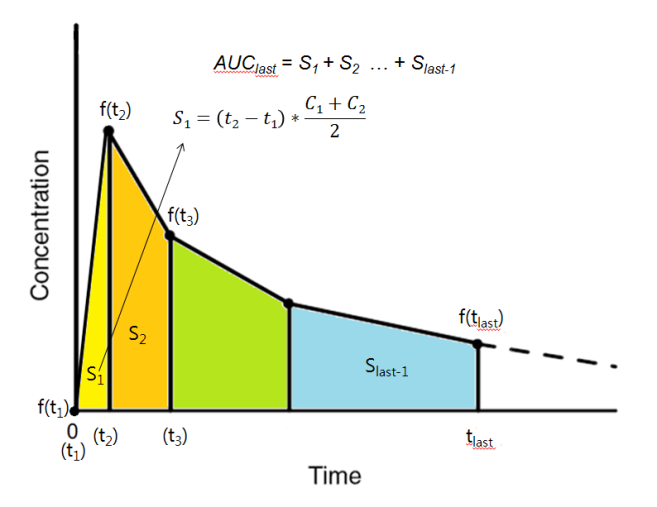
\includegraphics[width=1\linewidth]{assets/trapezoidal} \caption{Linear trapezoidal method}\label{fig:trapezoid}
\end{figure}

추가적으로 마지막으로 농도를 잰 시점에서 모든 약물이 우리 몸에서
빠져나가는 시점까지의 값을 구하기 위해서 마지막으로 측정한 점의 기울기가
그대로 약물이 모두 제거되는 시점까지 그대로 유지된다는 가정을 세우게
됩니다. 다음과 같이 C\textsubscript{last}(가장 마지막으로 농도를 측정한
시점)에서 λ (C\textsubscript{max} 이후에 선형성이 가장 높은 3점을
선택하여 구한 기울기)를 구한 후 다음과 같은 약동학 공식을 대입하여 값을
구해주게 됩니다.

\[
AUC_{t_{last}-\infty} = 
  \frac{C_{last}}{\lambda} \\
AUMC_{t_{last}-\infty} = 
  \frac{t_{last} \cdot C_{last}}{\lambda} + 
  \frac{C_{last}}{\lambda^2}
\]

약물이 우리 몸에 들어온 후 가장 높은 농도의 경우 실제 개개인에서 농도를
측정한 값들 중 가장 높은 농도를 실제 가장 높은 농도라 가정하여 사용하게
되고, 이 지표를 C\textsubscript{max}라 부릅니다. 또한 이때의 시점을
T\textsubscript{max}라 부르게 됩니다. 위에서 구한 AUC와
C\textsubscript{max}, λ 를 가지고 나머지 주요 값을 계산하게 됩니다. 이
중 청소율(제거되는 속도)에 해당하는 clearance(일반적으로 CL이라
지칭한다.) 의 경우 다음의 약동학 기본 공식을 활용하여 구해주게 됩니다.

\[
CL = \frac{D \cdot F}{AUC}
\]

수식에서 D는 dose로 투여량을, F는 생체이용률을 의미합니다.

우리 몸의 분포 (disposition)을 알기 위해 우리 몸의 volume을 나타내는
volume of distribution at steady state (Vdss)는 아래 식을 이용하여 값을
구하게 됩니다.

\[
Vd_{ss} = MRT \cdot CL = \frac{AUMC}{AUC} \cdot \frac{D}{AUC}
\]

우리 몸의 생체이용률을 나타내는 F의 경우 기본적으로 정맥주사시의
생체이용률을 1이라고 가정하고, 다음 식으로 구합니다.

\[
F = \frac{D_{iv}}{D_{oral}} \cdot \frac{AUC_{oral}}{AUC_{iv}}
\]

(이중 Div는 정맥주사 투여량, Doral은 경구 투여량, AUCoral은 경구
투여에서의 AUC, AUCiv는 정맥투여에서의 AUC를 의미한다. 이처럼 AUC,
C\textsubscript{max}, AUMC, λ 를 구하는 부분에 있어서는
non-compartmental analysis의 기본 가정들을 활용하였고 그 밖의
부분들에서는 현재 정형화된 공식들을 활용하여 적용하였다. 위 내용을
바탕으로 R을 기반으로 한 script를 구성한 후 전세계적으로 널리 쓰이고
있는 CDISC terminology를 각각의 지표들에 적용하여 결과값을 도출하였다.

또한 투여되는 방식을 3가지 분류(Extravascular, IV infusion, IV bolus)로
구분하여, 그에 맞는 각각의 식을 적용하였다. 마지막으로 시간당 농도의
변화율이 농도 증가 곡선보다 감소 곡선에서 완만하다는 점을 고려하여
농도가 감소하는 구간에서는 log값을 선택적으로 줄 수 있도록 설정하였으며,
흡수 속도 상수의 경우 현 NCA method를 통해 구하기에는 한계가 있어 따로
값을 제시하지 않았습니다.

흡수속도 상수를 구하기 위해서는 구획분석방법(compartmental analysis)이나
비선형 혼합모형(non-linear mixed effect modeling)을 사용하는 것이
바람직합니다.

Figure 2. Linear trapezoidal method를 적용한 AUC의 계산 Script

Figure 3 약동학 지표들에 대해 각각의 공식을 적용한 Script의 예

\chapter{R과 그 패키지에 대하여}\label{R-and-packages}

\section{이 장에서는}\label{summary-r-packages}

R (R Core Team \protect\hyperlink{ref-R-base}{2018})은 통계 소프트웨어
입니다. 특히 자료의 재현가능한 편집이라는 측면이 가장 중요합니다. 오류를
줄일 수 있고, 한번 설정한 것을 반복해서 적용하는 것이 쉽기 때문입니다.
이 책에서 주로 다루게 될 \texttt{NonCompart} (Bae
\protect\hyperlink{ref-R-NonCompart}{2018}\protect\hyperlink{ref-R-NonCompart}{b}),
\texttt{ncar} (Bae
\protect\hyperlink{ref-R-ncar}{2018}\protect\hyperlink{ref-R-ncar}{a}),
\texttt{pkr} (Bae and Lee \protect\hyperlink{ref-R-pkr}{2018}) 은 비구획
분석을 R을 통해 쉽고 빠르게 (매우 빠르게) 행할 수 있는 R 패키지입니다.

\texttt{NonCompart}의 패키지 제목은 Noncompartmental Analysis for
Pharmacokinetic Data, \texttt{ncar}의 패키지 제목은 Noncompartmental
Analysis for Pharmacokinetic Report, \texttt{pkr}의 패키지 제목은
Pharmacokinetics in R 입니다.

\section{R에 대하여}\label{basic}

굉장히 유용한 소프트웨어이지만 이에 대해 여기서 자세히 설명하긴
힘듭니다. R에 대한 많은 책들을 bookdown.org\footnote{\url{https://bookdown.org}}에서
무료로 읽을 수 있습니다. Coursera\footnote{\url{https://coursera.com}}에서
무료 온라인 강의를 들을 수 있습니다.

\section{설치}\label{install}

우선 R을 설치합니다. R은 아래 링크\footnote{\url{https://cran.r-project.org/}}에서
다운로드 받을 수 있습니다.

R을 실행한 후, 콘솔 창에서 비구획분석을 위한 패키지를 설치하는 방법은
다음과 같습니다. 홑따옴표 등의 인용 부호에 주의하세요.

\begin{Shaded}
\begin{Highlighting}[]
\KeywordTok{install.packages}\NormalTok{(}\StringTok{'NonCompart'}\NormalTok{)}
\KeywordTok{install.packages}\NormalTok{(}\StringTok{'ncar'}\NormalTok{)}
\KeywordTok{install.packages}\NormalTok{(}\StringTok{'pkr'}\NormalTok{)}
\end{Highlighting}
\end{Shaded}

설치는 한번만 하면 되지만, 비구획분석을 위해서는 매 세션마다 패키지를
\emph{불러오기}해야 합니다.

\begin{Shaded}
\begin{Highlighting}[]
\KeywordTok{library}\NormalTok{(NonCompart)}
\KeywordTok{library}\NormalTok{(ncar)}
\KeywordTok{library}\NormalTok{(pkr)}
\end{Highlighting}
\end{Shaded}

\section{기타 설치}\label{-}

아래 두 패키지는 비구획분석과는 관계없지만 자료 처리 혹은 그림 등을
그리는데 도움을 줍니다.

\begin{Shaded}
\begin{Highlighting}[]
\KeywordTok{library}\NormalTok{(ggplot2) }
\KeywordTok{library}\NormalTok{(dplyr) }
\KeywordTok{library}\NormalTok{(knitr) }
\end{Highlighting}
\end{Shaded}

도움이 필요할때는 맨 앞에 물음표를 붙여서 콘솔창에 입력하거나
\texttt{help()} 함수를 사용합니다.

\begin{Shaded}
\begin{Highlighting}[]
\NormalTok{?NonCompart}
\KeywordTok{help}\NormalTok{(tblNCA)}
\end{Highlighting}
\end{Shaded}

자료 분석을 위해 몇가지 도구가 필요한데 \texttt{tidyverse}(Wickham
\protect\hyperlink{ref-R-tidyverse}{2017})를 설치하면 다수의 편리한
패키지 \texttt{tidyr} (Wickham and Henry
\protect\hyperlink{ref-R-tidyr}{2018}), \texttt{dplyr} (Wickham et al.
\protect\hyperlink{ref-R-dplyr}{2018}), \texttt{tibble} (Müller and
Wickham \protect\hyperlink{ref-R-tibble}{2018}), \texttt{ggplot2}
{[}R-ggplot2{]}, \texttt{purrr} (Henry and Wickham
\protect\hyperlink{ref-R-purrr}{2018}), \texttt{readr} (Wickham, Hester,
and Francois \protect\hyperlink{ref-R-readr}{2017})의 설치와 불러오기
과정을 쉽게 끝낼 수 있습니다.

다만 비구획분석을 위한 함수의 입력을 위해 \texttt{tibble} 형식은
\texttt{as.data.frame()}을 통하여 데이타프레임으로 자료 형식을 변환하는
것이 좋습니다. 마찬가지로 \texttt{readr} 패키지의 \texttt{read\_csv()}
명령어를 쓸 경우 \texttt{tibble}로 읽혀지기 때문에
\texttt{as.data.frame()}으로 바꿔주거나 처음부터 \texttt{read\_csv()}를
쓰는 것을 고려할 수 있습니다.

\begin{Shaded}
\begin{Highlighting}[]
\KeywordTok{install.packages}\NormalTok{(}\StringTok{'devtools'}\NormalTok{)}
\NormalTok{devtools}\OperatorTok{::}\KeywordTok{install_github}\NormalTok{(}\StringTok{'tidyverse/tidyverse'}\NormalTok{)}
\KeywordTok{library}\NormalTok{(tidyverse)}
\end{Highlighting}
\end{Shaded}

\chapter{기본 자료}\label{datasets}

\section{이 장에서는}\label{introdatasets}

R에는 theophylline과 Indomethacin의 약동학 데이터가 내장되어 있습니다.

\begin{itemize}
\tightlist
\item
  \texttt{Theoph}: theophylline의 약동학 데이터, 12명, 320mg PO
  단회투여, 0\textasciitilde{}24시간 채혈, NONMEM 의 run 폴더의 THEOPP
  데이터와 동일합니다.
\item
  \texttt{Indometh}: Indomethacin의 약동학 데이터, 6명, 25mg IV bolus
  단회투여, 0\textasciitilde{}8시간 채혈(0, 0.25, 0.5, 0.75, 1, 1.25, 2,
  3, 4, 5, 6, 8 h) (데이터명의 첫글짜가 대문자임에 주의하길)
\end{itemize}

먼저 데이터를 살펴보겠습니다.

\section{데이타에 대해}\label{TheophData}

Theoph 자료의 첫 10개 (Table \ref{tab:head}) 혹은 마지막 10개 관찰값만
보고 싶으면 다음을 입력합니다. 대상자 번호가 첫 열에 나와있고 시간
순서대로 혈장에서 측정한 테오필린의 농도가 나와있습니다.

\begin{Shaded}
\begin{Highlighting}[]
\KeywordTok{head}\NormalTok{(Theoph, }\DataTypeTok{n=}\DecValTok{10}\NormalTok{)}
\KeywordTok{tail}\NormalTok{(Theoph, }\DataTypeTok{n=}\DecValTok{10}\NormalTok{)}
\end{Highlighting}
\end{Shaded}

\begin{table}

\caption{\label{tab:head}Theoph 자료의 첫 10개 관찰값}
\centering
\begin{tabular}[t]{lrrrr}
\toprule
Subject & Wt & Dose & Time & conc\\
\midrule
1 & 79.6 & 4.02 & 0.00 & 0.74\\
1 & 79.6 & 4.02 & 0.25 & 2.84\\
1 & 79.6 & 4.02 & 0.57 & 6.57\\
1 & 79.6 & 4.02 & 1.12 & 10.50\\
1 & 79.6 & 4.02 & 2.02 & 9.66\\
\addlinespace
1 & 79.6 & 4.02 & 3.82 & 8.58\\
1 & 79.6 & 4.02 & 5.10 & 8.36\\
1 & 79.6 & 4.02 & 7.03 & 7.47\\
1 & 79.6 & 4.02 & 9.05 & 6.89\\
1 & 79.6 & 4.02 & 12.12 & 5.94\\
\bottomrule
\end{tabular}
\end{table}

그림을 그려서 대략적인 자료의 모습을 파악합니다. (Figure
\ref{fig:ggtheoph})

\begin{Shaded}
\begin{Highlighting}[]
\KeywordTok{ggplot}\NormalTok{(Theoph, }\KeywordTok{aes}\NormalTok{(Time, conc, }\DataTypeTok{group =}\NormalTok{ Subject, }\DataTypeTok{color =}\NormalTok{ Subject)) }\OperatorTok{+}
\StringTok{  }\KeywordTok{geom_point}\NormalTok{(}\DataTypeTok{size =} \DecValTok{4}\NormalTok{) }\OperatorTok{+}\StringTok{ }
\StringTok{  }\KeywordTok{geom_line}\NormalTok{(}\DataTypeTok{size =} \DecValTok{1}\NormalTok{) }\OperatorTok{+}
\StringTok{  }\KeywordTok{theme_bw}\NormalTok{() }\OperatorTok{+}
\StringTok{  }\KeywordTok{labs}\NormalTok{(}\DataTypeTok{title =} \StringTok{'Oral Administration of Theoph (320 mg)'}\NormalTok{,}
       \DataTypeTok{x =} \StringTok{'Time (hour)'}\NormalTok{, }\DataTypeTok{y =} \StringTok{'Concentration (ng/mL)'}\NormalTok{)}
\end{Highlighting}
\end{Shaded}

\begin{figure}
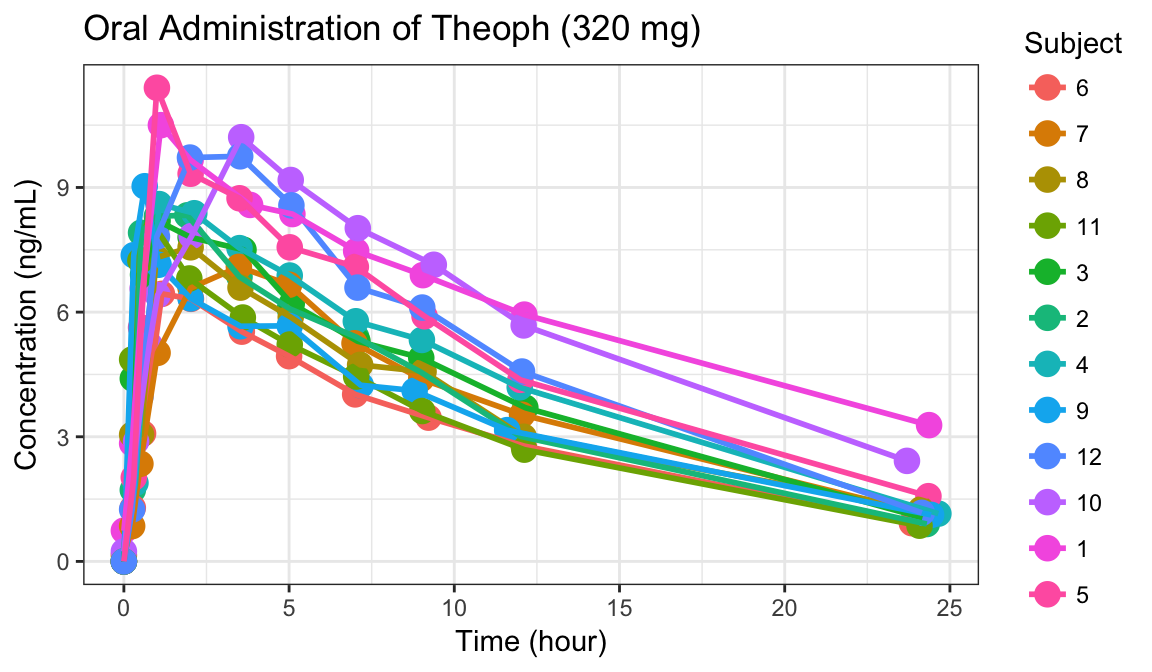
\includegraphics[width=1\linewidth]{book-ncar_files/figure-latex/ggtheoph-1} \caption{Concentration-time curves of oral administration of Theoph (N = 12)}\label{fig:ggtheoph}
\end{figure}

데이터가 Subject, weight, Dose, Time, Concentration 으로 구성되었음을 알
수 있습니다.

\chapter{R을 사용한 비구획분석}\label{noncompart}

\section{이 장에서는}\label{summary-noncompart}

\texttt{NonCompart} (Bae
\protect\hyperlink{ref-R-NonCompart}{2018}\protect\hyperlink{ref-R-NonCompart}{b})은
비구획 분석을 R을 통해 쉽고 빠르게 (매우 빠르게) 행할 수 있는
패키지입니다. 약동학 교재의 내용을 충실히 반영하였습니다. (Gabrielsson
\protect\hyperlink{ref-gab}{2016}; Rowland
\protect\hyperlink{ref-tozer}{2011}) 이에 대해 좀더 자세히
알아보겠습니다.

\texttt{NonCompart}의 \texttt{DESCRIPTION} 파일을 보면 다음과 같이
설명하고 있습니다.

\begin{quote}
Conduct a noncompartmental analysis as closely as possible to the most
widely used commercial software for pharmacokinetic analysis, i.e.
`Phoenix(R) WinNonlin(R)'
\url{https://www.certara.com/software/pkpd-modeling-and-simulation/phoenix-winnonlin/}.
Some features are 1) Use of CDISC SDTM terms 2) Automatic slope
selection with the same criterion of WinNonlin(R) 3) Supporting both
`linear-up linear-down' and `linear-up log-down' method 4)
Interval(partial) AUCs with `linear' or `log' interpolation method *
Reference: Gabrielsson J, Weiner D. Pharmacokinetic and Pharmacodynamic
Data Analysis - Concepts and Applications. 5th ed. 2016.
(\url{ISBN:9198299107}).
\end{quote}

\begin{Shaded}
\begin{Highlighting}[]
\KeywordTok{library}\NormalTok{(tidyverse)}
\KeywordTok{library}\NormalTok{(NonCompart)}
\KeywordTok{library}\NormalTok{(ncar)}
\end{Highlighting}
\end{Shaded}

\section{NonCompart 사용법}\label{how-to-use}

tblNCA의 사용법은 다음과 같습니다.

\begin{verbatim}
## function (concData, key = "Subject", colTime = "Time", colConc = "conc", 
##     dose = 0, adm = "Extravascular", dur = 0, doseUnit = "mg", 
##     timeUnit = "h", concUnit = "ug/L", down = "Linear", R2ADJ = 0.9, 
##     MW = 0) 
## NULL
\end{verbatim}

concData는 데이터셋을 설정하며, \texttt{key}는 subject ID의 컬럼명 혹은
treatment code의 컬럼명(교차시험에서 사용), \texttt{colTime}은 time의
컬럼명, \texttt{colConc}는 concentration의 컬럼명 등을 함수 인자로
갖습니다. 그 외 인자들에 대해서 살펴보자면 다음과 같습니다.

\begin{enumerate}
\def\labelenumi{\arabic{enumi}.}
\tightlist
\item
  \texttt{down}

  \begin{itemize}
  \tightlist
  \item
    AUC와 AUMC를 구하는 trapezoidal method 설정이며, 기본값은
    \texttt{Linear}입니다.
  \item
    \texttt{Linear}와 \texttt{Log} 중 선택 가능하며 각각 linear
    trapezoidal method와 linear-up and log-down method를 의미합니다.
  \end{itemize}
\item
  \texttt{dose}

  \begin{itemize}
  \tightlist
  \item
    투여량에 대한 설정입니다. 단위에 주의해야 합니다. 벡터값을 줌으로서
    각 대상자별 용량을 다르게 할 수 있습니다.
  \end{itemize}
\item
  \texttt{adm}

  \begin{itemize}
  \tightlist
  \item
    투여경로에 대한 설정, 기본값은 ``Extravascular''으로 경구 투여 등을
    의미합니다.
  \item
    Bolus, Infusion, Extravascular 중에서 선택 가능하다.
  \end{itemize}
\item
  \texttt{dur}

  \begin{itemize}
  \tightlist
  \item
    주입하는 기간(infusion duration)을 설정합니다. 기본값은 0입니다.
  \end{itemize}
\item
  \texttt{R2ADJ}

  \begin{itemize}
  \tightlist
  \item
    \texttt{R2ADJ} 값이 설정값 이하인 경우 \texttt{DetSlope()}함수에
    의해 terminal slope를 수동으로 interactive하게 고를 수 있게됩니다.
  \end{itemize}
\end{enumerate}

이제 약동학 파라미터를 산출하기 위해서는 아래와 같이 하면 됩니다. 우선
Theophylline 의 약동학 파라미터를 구해보겠습니다.

\begin{Shaded}
\begin{Highlighting}[]
\NormalTok{TheophNca <-}\StringTok{ }\NormalTok{NonCompart}\OperatorTok{::}\KeywordTok{tblNCA}\NormalTok{(Theoph, }\StringTok{"Subject"}\NormalTok{, }\StringTok{"Time"}\NormalTok{, }\StringTok{"conc"}\NormalTok{, }\DataTypeTok{dose=}\DecValTok{320}\NormalTok{, }\DataTypeTok{concUnit=}\StringTok{"mg/L"}\NormalTok{)}
\KeywordTok{head}\NormalTok{(TheophNca)}
\end{Highlighting}
\end{Shaded}

\begin{verbatim}
##   Subject       b0  CMAX      CMAXD TMAX TLAG CLST     CLSTP  TLST
## 1       1 2.368785 10.50 0.03281250 1.12    0 3.28 3.2801465 24.37
## 2       2 2.411237  8.33 0.02603125 1.92    0 0.90 0.8886398 24.30
## 3       3 2.529712  8.20 0.02562500 1.02    0 1.05 1.0550967 24.17
## 4       4 2.592755  8.60 0.02687500 1.07    0 1.15 1.1564216 24.65
## 5       5 2.551092 11.40 0.03562500 1.00    0 1.57 1.5556951 24.35
## 6       6 2.033404  6.44 0.02012500 1.15    0 0.92 0.9412712 23.85
##      LAMZHL       LAMZ LAMZLL LAMZUL LAMZNPT     CORRXY        R2
## 1 14.304378 0.04845700   9.05  24.37       3 -0.9999999 0.9999997
## 2  6.659342 0.10408644   7.03  24.30       4 -0.9985967 0.9971954
## 3  6.766087 0.10244431   9.00  24.17       3 -0.9996624 0.9993250
## 4  6.981247 0.09928702   9.02  24.65       3 -0.9994619 0.9989241
## 5  8.002264 0.08661888   7.02  24.35       4 -0.9993234 0.9986472
## 6  7.894998 0.08779574   2.03  23.85       7 -0.9991203 0.9982413
##       R2ADJ    AUCLST    AUCALL    AUCIFO   AUCIFOD   AUCIFP   AUCIFPD
## 1 0.9999995 148.92305 148.92305 216.61193 0.6769123 216.6150 0.6769217
## 2 0.9957931  91.52680  91.52680 100.17346 0.3130421 100.0643 0.3127010
## 3 0.9986499  99.28650  99.28650 109.53597 0.3422999 109.5857 0.3424554
## 4 0.9978483 106.79630 106.79630 118.37888 0.3699340 118.4436 0.3701361
## 5 0.9979708 121.29440 121.29440 139.41978 0.4356868 139.2546 0.4351707
## 6 0.9978896  73.77555  73.77555  84.25442 0.2632951  84.4967 0.2640522
##      AUCPEO    AUCPEP   AUMCLST   AUMCIFO   AUMCIFP  AUMCPEO  AUMCPEP
## 1 31.248917 31.249876 1459.0711 4505.5348 4505.6709 67.61603 67.61701
## 2  8.631687  8.532030  706.5866  999.7723  996.0716 29.32525 29.06267
## 3  9.357173  9.398325  803.1859 1150.9648 1152.6529 30.21629 30.31850
## 4  9.784331  9.833594  901.0842 1303.2524 1305.4981 30.85881 30.97775
## 5 13.000579 12.897403 1017.1143 1667.7216 1661.7937 39.01174 38.79419
## 6 12.437174 12.688246  609.1524  978.4285  986.9665 37.74176 38.28034
##       VZFO     VZFP     CLFO     CLFP MRTEVLST  MRTEVIFO  MRTEVIFP
## 1 30.48675 30.48632 1.477296 1.477276 9.797483 20.800031 20.800368
## 2 30.69044 30.72392 3.194459 3.197943 7.719996  9.980411  9.954313
## 3 28.51710 28.50415 2.921415 2.920088 8.089578 10.507642 10.518276
## 4 27.22596 27.21110 2.703185 2.701709 8.437410 11.009163 11.022112
## 5 26.49799 26.52942 2.295227 2.297949 8.385501 11.961873 11.933490
## 6 43.25973 43.13569 3.798020 3.787130 8.256833 11.612785 11.680533
\end{verbatim}

여기서 \texttt{dose=320}으로 되었다는 것은 아미노필린 400mg 투여시
테오필린 320mg이 체내로 들어감을 의미합니다.

이는 문자(character)로 구성된 matrix로 구성된 결과물과 단위 정보가 담긴
attribute를 포함하고 있습니다.

다음으로 Indomethacin 의 약동학 파라미터를 구해보자. 이는 IV bolus
이므로 AdmMode 옵션이 추가됩니다.

\begin{Shaded}
\begin{Highlighting}[]
\NormalTok{NonCompart}\OperatorTok{::}\KeywordTok{tblNCA}\NormalTok{(Indometh, }\StringTok{"Subject"}\NormalTok{, }\StringTok{"time"}\NormalTok{, }\StringTok{"conc"}\NormalTok{, }\DataTypeTok{dose=}\DecValTok{25}\NormalTok{, }\DataTypeTok{adm=}\StringTok{"Bolus"}\NormalTok{, }\DataTypeTok{dur=}\FloatTok{0.5}\NormalTok{, }\DataTypeTok{concUnit=}\StringTok{"mg/L"}\NormalTok{)}
\end{Highlighting}
\end{Shaded}

\begin{verbatim}
##   Subject         b0 CMAX  CMAXD TMAX TLAG CLST      CLSTP TLST   LAMZHL
## 1       1 -1.7242106 1.50 0.0600 0.25   NA 0.05 0.05024851    8 4.378127
## 2       2 -0.1752869 2.03 0.0812 0.25   NA 0.08 0.07475591    8 2.293063
## 3       3         NA 2.72 0.1088 0.25   NA 0.08         NA    8       NA
## 4       4         NA 1.85 0.0740 0.25   NA 0.07         NA    8       NA
## 5       5         NA 2.05 0.0820 0.25   NA 0.06         NA    8       NA
## 6       6         NA 2.31 0.0924 0.25   NA 0.09         NA    8       NA
##        LAMZ LAMZLL LAMZUL LAMZNPT     CORRXY        R2     R2ADJ   AUCLST
## 1 0.1583205   5.00      8       3 -0.9985323 0.9970667 0.9941335 2.040452
## 2 0.3022800   0.75      8       9 -0.9734830 0.9476691 0.9401933 3.248520
## 3        NA     NA     NA       0         NA        NA        NA 3.554421
## 4        NA     NA     NA       0         NA        NA        NA 2.785279
## 5        NA     NA     NA       0         NA        NA        NA 2.458858
## 6        NA     NA     NA       0         NA        NA        NA 3.335703
##     AUCALL   AUCIFO    AUCIFOD   AUCIFP    AUCIFPD    AUCPEO    AUCPEP
## 1 2.040452 2.356267 0.09425069 2.357837 0.09431348 13.403196 13.460844
## 2 3.248520 3.513175 0.14052701 3.495827 0.13983307  7.533221  7.074344
## 3 3.554421       NA         NA       NA         NA        NA        NA
## 4 2.785279       NA         NA       NA         NA        NA        NA
## 5 2.458858       NA         NA       NA         NA        NA        NA
## 6 3.335703       NA         NA       NA         NA        NA        NA
##    AUMCLST  AUMCIFO  AUMCIFP  AUMCPEO  AUMCPEP       C0  AUCPBEO  AUCPBEP
## 1 3.271250 7.792554 7.815026 58.02083 58.14153 2.393617 20.65564 20.64189
## 2 6.398750 9.391522 9.195343 31.86674 30.41314 2.528160 16.21809 16.29857
## 3 5.006250       NA       NA       NA       NA 4.965369       NA       NA
## 4 4.381875       NA       NA       NA       NA 2.462230       NA       NA
## 5 3.707500       NA       NA       NA       NA 4.040865       NA       NA
## 6 5.532500       NA       NA       NA       NA 3.705625       NA       NA
##        VZO      VZP      CLO       CLP MRTIVLST MRTIVIFO MRTIVIFP     VSSO
## 1 67.01598 66.97136 10.61000 10.602939 1.353199 3.057161 3.064490 32.43648
## 2 23.54132 23.65814  7.11607  7.151384 1.719743 2.423229 2.380377 17.24387
## 3       NA       NA       NA        NA 1.158457       NA       NA       NA
## 4       NA       NA       NA        NA 1.323227       NA       NA       NA
## 5       NA       NA       NA        NA 1.257814       NA       NA       NA
## 6       NA       NA       NA        NA 1.408571       NA       NA       NA
##       VSSP
## 1 32.49260
## 2 17.02299
## 3       NA
## 4       NA
## 5       NA
## 6       NA
\end{verbatim}

\section{구간 NCA}\label{interval-NCA}

\begin{enumerate}
\def\labelenumi{\arabic{enumi}.}
\tightlist
\item
  iAUC

  \begin{itemize}
  \tightlist
  \item
    일부구간에 대한 AUC를 구하기 위한 구간설정 옵션입니다.
  \item
    ``Name'', ``Start'', ``End'' 3개의 컬럼으로 구성된 데이터 프레임으로
    설정해야 합니다.
  \end{itemize}
\end{enumerate}

일부 구간의 AUC를 구하는 방법은 조금 더 복잡하므로 자세히 알아봅시다.
예를 들어 0\textasciitilde{}12시간까지의 AUC,
0\textasciitilde{}24시간까지의 AUC를 구하고자 한다면 다음과 같이 하면
됩니다. 먼저 구하고자 하는 구간에 대한 정보를 갖는 변수를 아래와같이
생성합니다.

\begin{Shaded}
\begin{Highlighting}[]
\NormalTok{iAUC <-}\StringTok{ }\KeywordTok{data.frame}\NormalTok{(}\DataTypeTok{Name=}\KeywordTok{c}\NormalTok{(}\StringTok{"AUC[0-12h]"}\NormalTok{,}\StringTok{"AUC[0-24h]"}\NormalTok{), }\DataTypeTok{Start=}\KeywordTok{c}\NormalTok{(}\DecValTok{0}\NormalTok{,}\DecValTok{0}\NormalTok{), }\DataTypeTok{End=}\KeywordTok{c}\NormalTok{(}\DecValTok{12}\NormalTok{,}\DecValTok{24}\NormalTok{)) ; iAUC}
\end{Highlighting}
\end{Shaded}

\begin{verbatim}
##         Name Start End
## 1 AUC[0-12h]     0  12
## 2 AUC[0-24h]     0  24
\end{verbatim}

\begin{verbatim}
    Name Start End
\end{verbatim}

1 AUC{[}0-12h{]} 0 12 2 AUC{[}0-24h{]} 0 24

이제 iAUC 옵션을 이용해서 이를 구합니다.

\begin{Shaded}
\begin{Highlighting}[]
\CommentTok{# tblNCA(Theoph, "Subject", "Time", "conc", dose=320, iAUC=iAUC)}
\end{Highlighting}
\end{Shaded}

맨 마지막 파라미터로 AUC{[}0-12h{]}, AUC{[}0-24h{]}가 추가되었음을 알 수
있습니다.

개인별 일부 구간의 AUC를 구하는 방법은 아래와 같다. 예를 들어
0\textasciitilde{}12시간까지의 AUC, 0\textasciitilde{}24시간까지의 AUC를
구하고자 한다면 다음과 같이 하면 된다.

\begin{quote}
iAUC = data.frame(Name=c(``AUC{[}0-12h{]}'',``AUC{[}0-24h{]}''),
Start=c(0,0), End=c(12,24)) ; iAUC
\end{quote}

\begin{verbatim}
    Name Start End
\end{verbatim}

1 AUC{[}0-12h{]} 0 12 2 AUC{[}0-24h{]} 0 24

\begin{Shaded}
\begin{Highlighting}[]
\CommentTok{#IntAUC}
\CommentTok{#IntAUC(Theoph[Theoph$Subject==1,"Time"], Theoph[Theoph$Subject==1, "conc"], Dose=320, iAUC=iAUC)}
\end{Highlighting}
\end{Shaded}

\begin{verbatim}
        CMAX        CMAXD         TMAX         TLAG         CLST        CLSTP         TLST       LAMZHL         LAMZ 
  10.5000000    0.0328125    1.1200000    0.0000000    3.2800000    3.2801465   24.3700000   14.3043776    0.0484570 
      LAMZLL       LAMZUL      LAMZNPT       CORRXY           R2        R2ADJ       AUCLST       AUCALL       AUCIFO 
   9.0500000   24.3700000    3.0000000   -0.9999999    0.9999997    0.9999995  148.9230500  148.9230500  216.6119330 
     AUCIFOD       AUCPEO       AUCIFP      AUCIFPD       AUCPEP      AUMCLST      AUMCIFO      AUMCPEO      AUMCIFP 
   0.6769123   31.2489169  216.6149558    0.6769217   31.2498763 1459.0711035 4505.5348194   67.6160287 4505.6708646 
     AUMCPEP     MRTEVLST     MRTEVIFO     MRTEVIFP         VZFO         VZFP         CLFO         CLFP   AUC[0-12h] 
  67.6170065    9.7974834   20.8000305   20.8003683   30.4867482   30.4863228    1.4772963    1.4772757   91.7355220 
  AUC[0-24h] 
 147.6945866 
\end{verbatim}

김민걸 선생님 자료를 옮겨와서 변형합니다.
\url{http://blog.naver.com/kimmingul}

\section{함수 살펴보기}\label{functions}

NonCompart 패키지 내의 여러가지 함수를 살펴보겠습니다. AUC(),
BestSlope(), DetSlope(), IntAUC(), Interpol(), LinAUC(), LogAUC(),
Slope(), sNCA(), tblNCA(), Unit(), UnitUrine(), UT()라는 함수가
있습니다.

\subsection{AUC}\label{auc}

AUC와 AUMC를 `Linear trapezoidal method' 혹은 'linear-up and log-down
method'의 두가지 방식으로 계산하게 됩니다.

\begin{Shaded}
\begin{Highlighting}[]
\KeywordTok{AUC}\NormalTok{(Theoph[Theoph}\OperatorTok{$}\NormalTok{Subject}\OperatorTok{==}\DecValTok{1}\NormalTok{, }\StringTok{"Time"}\NormalTok{], Theoph[Theoph}\OperatorTok{$}\NormalTok{Subject}\OperatorTok{==}\DecValTok{1}\NormalTok{, }\StringTok{"conc"}\NormalTok{])}
\end{Highlighting}
\end{Shaded}

\begin{verbatim}
##            [,1]        [,2]
##  [1,]   0.00000    0.000000
##  [2,]   0.44750    0.088750
##  [3,]   1.95310    0.801534
##  [4,]   6.64735    5.065382
##  [5,]  15.71935   19.138321
##  [6,]  32.13535   66.198241
##  [7,]  42.97695  114.461665
##  [8,]  58.25290  206.281512
##  [9,]  72.75650  322.298798
## [10,]  92.45055  528.521903
## [11,] 148.92305 1459.071104
\end{verbatim}

\begin{Shaded}
\begin{Highlighting}[]
\KeywordTok{AUC}\NormalTok{(Theoph[Theoph}\OperatorTok{$}\NormalTok{Subject}\OperatorTok{==}\DecValTok{1}\NormalTok{, }\StringTok{"Time"}\NormalTok{], Theoph[Theoph}\OperatorTok{$}\NormalTok{Subject}\OperatorTok{==}\DecValTok{1}\NormalTok{, }\StringTok{"conc"}\NormalTok{], }\DataTypeTok{down=}\StringTok{"Log"}\NormalTok{)}
\end{Highlighting}
\end{Shaded}

\begin{verbatim}
##            [,1]        [,2]
##  [1,]   0.00000    0.000000
##  [2,]   0.44750    0.088750
##  [3,]   1.95310    0.801534
##  [4,]   6.64735    5.065382
##  [5,]  15.71410   19.243482
##  [6,]  32.11090   66.830600
##  [7,]  42.95189  115.151380
##  [8,]  58.21173  207.426110
##  [9,]  72.70744  323.774418
## [10,]  92.36544  531.108538
## [11,] 147.23475 1499.129085
\end{verbatim}

\section{긴 형식으로 변환하면서 단위 추가하기}\label{long-format}

NonCompart 패키지의 tblNCA()함수를 사용해서 비구획분석 결과를 내면
문자형식의 행렬이 생성되고 그 attr로 dimnames와 units를 갖는데 이를 long
format의 tidy data로 변환하는 방법은 다음과 같습니다.

\begin{Shaded}
\begin{Highlighting}[]
\NormalTok{ncares <-}\StringTok{ }\NormalTok{NonCompart}\OperatorTok{::}\KeywordTok{tblNCA}\NormalTok{(Theoph, }\DataTypeTok{key=}\StringTok{"Subject"}\NormalTok{, }\DataTypeTok{dose=}\DecValTok{320}\NormalTok{, }\DataTypeTok{concUnit=}\StringTok{"mg/L"}\NormalTok{)}
\KeywordTok{str}\NormalTok{(ncares)}
\end{Highlighting}
\end{Shaded}

\begin{verbatim}
## 'data.frame':    12 obs. of  37 variables:
##  $ Subject : Ord.factor w/ 12 levels "6"<"7"<"8"<"11"<..: 11 6 5 7 12 1 2 3 8 10 ...
##  $ b0      : num  2.37 2.41 2.53 2.59 2.55 ...
##  $ CMAX    : num  10.5 8.33 8.2 8.6 11.4 ...
##  $ CMAXD   : num  0.0328 0.026 0.0256 0.0269 0.0356 ...
##  $ TMAX    : num  1.12 1.92 1.02 1.07 1 1.15 3.48 2.02 0.63 3.55 ...
##  $ TLAG    : num  0 0 0 0 0 0 0 0 0 0 ...
##  $ CLST    : num  3.28 0.9 1.05 1.15 1.57 0.92 1.15 1.25 1.12 2.42 ...
##  $ CLSTP   : num  3.28 0.889 1.055 1.156 1.556 ...
##  $ TLST    : num  24.4 24.3 24.2 24.6 24.4 ...
##  $ LAMZHL  : num  14.3 6.66 6.77 6.98 8 ...
##  $ LAMZ    : num  0.0485 0.1041 0.1024 0.0993 0.0866 ...
##  $ LAMZLL  : num  9.05 7.03 9 9.02 7.02 2.03 6.98 3.53 8.8 9.38 ...
##  $ LAMZUL  : num  24.4 24.3 24.2 24.6 24.4 ...
##  $ LAMZNPT : num  3 4 3 3 4 7 4 6 3 3 ...
##  $ CORRXY  : num  -1 -0.999 -1 -0.999 -0.999 ...
##  $ R2      : num  1 0.997 0.999 0.999 0.999 ...
##  $ R2ADJ   : num  1 0.996 0.999 0.998 0.998 ...
##  $ AUCLST  : num  148.9 91.5 99.3 106.8 121.3 ...
##  $ AUCALL  : num  148.9 91.5 99.3 106.8 121.3 ...
##  $ AUCIFO  : num  217 100 110 118 139 ...
##  $ AUCIFOD : num  0.677 0.313 0.342 0.37 0.436 ...
##  $ AUCIFP  : num  217 100 110 118 139 ...
##  $ AUCIFPD : num  0.677 0.313 0.342 0.37 0.435 ...
##  $ AUCPEO  : num  31.25 8.63 9.36 9.78 13 ...
##  $ AUCPEP  : num  31.25 8.53 9.4 9.83 12.9 ...
##  $ AUMCLST : num  1459 707 803 901 1017 ...
##  $ AUMCIFO : num  4506 1000 1151 1303 1668 ...
##  $ AUMCIFP : num  4506 996 1153 1305 1662 ...
##  $ AUMCPEO : num  67.6 29.3 30.2 30.9 39 ...
##  $ AUMCPEP : num  67.6 29.1 30.3 31 38.8 ...
##  $ VZFO    : num  30.5 30.7 28.5 27.2 26.5 ...
##  $ VZFP    : num  30.5 30.7 28.5 27.2 26.5 ...
##  $ CLFO    : num  1.48 3.19 2.92 2.7 2.3 ...
##  $ CLFP    : num  1.48 3.2 2.92 2.7 2.3 ...
##  $ MRTEVLST: num  9.8 7.72 8.09 8.44 8.39 ...
##  $ MRTEVIFO: num  20.8 9.98 10.51 11.01 11.96 ...
##  $ MRTEVIFP: num  20.8 9.95 10.52 11.02 11.93 ...
##  - attr(*, "units")= chr  "" "" "mg/L" "mg/L/mg" ...
\end{verbatim}

\begin{Shaded}
\begin{Highlighting}[]
\KeywordTok{left_join}\NormalTok{(}\KeywordTok{as_tibble}\NormalTok{(ncares) }\OperatorTok\StringTok{ }\NormalTok{tidyr}\OperatorTok{::}\KeywordTok{gather}\NormalTok{(PPTESTCD, PPORRES, }\OperatorTok{-}\NormalTok{Subject),}
          \KeywordTok{tibble}\NormalTok{(}\DataTypeTok{PPTESTCD =} \KeywordTok{attr}\NormalTok{(ncares, }\StringTok{'dimnames'}\NormalTok{)[[}\DecValTok{2}\NormalTok{]], }\DataTypeTok{UNIT =} \KeywordTok{attr}\NormalTok{(ncares, }\StringTok{'units'}\NormalTok{)),}
          \DataTypeTok{by =} \StringTok{'PPTESTCD'}\NormalTok{) }\OperatorTok\StringTok{ }
\StringTok{  }\KeywordTok{arrange}\NormalTok{(Subject, PPTESTCD) }\OperatorTok\StringTok{ }
\StringTok{  }\KeywordTok{head}\NormalTok{(}\DecValTok{20}\NormalTok{)}
\end{Highlighting}
\end{Shaded}

\begin{verbatim}
## Error: Column `PPTESTCD` must be a 1d atomic vector or a list
\end{verbatim}

\chapter{R을 사용한 비구획분석 보고서}\label{ncar}

\section{이 장에서는}\label{summary-ncar}

보고서를 일정한 형식으로 작성하여 다른 사람/기관과 공유하는 것은
중요합니다. 이를 \texttt{ncar} 패키지를 사용하여 좀더 쉽게 할 수
있습니다. 이 패키지를 통해서 약동학 파라이터를 보고서 형식의 text, pdf,
rtf 파일로 저장할 수 있습니다. 이에 대해 좀더 자세히 알아보겠습니다.

\texttt{ncar}의 \texttt{DESCRIPTION} 파일을 보면 다음과 같이 설명하고
있습니다.

\begin{quote}
Conduct a noncompartmental analysis as closely as possible to the most
widely used commercial software for pharmacokinetic analysis, i.e.
`Phoenix(R) WinNonlin(R)'
\url{https://www.certara.com/software/pkpd-modeling-and-simulation/phoenix-winnonlin/}.
Some features are 1) CDISC SDTM terms 2) Automatic slope selection with
the same criterion of WinNonlin(R) 3) Supporting both `linear-up
linear-down' and `linear-up log-down' method 4) Interval(partial) AUCs
with `linear' or `log' interpolation method 5) Produce pdf, rtf, text
report files. * Reference: Gabrielsson J, Weiner D. Pharmacokinetic and
Pharmacodynamic Data Analysis - Concepts and Applications. 5th ed. 2016.
(\url{ISBN:9198299107}).
\end{quote}

\begin{Shaded}
\begin{Highlighting}[]
\KeywordTok{library}\NormalTok{(tidyverse)}
\KeywordTok{library}\NormalTok{(ncar)}
\end{Highlighting}
\end{Shaded}

\section{ncar 사용법}\label{ncar-}

우선 저장될 폴더를 확인하면 다음과 같습니다.

\begin{Shaded}
\begin{Highlighting}[]
\KeywordTok{getwd}\NormalTok{()}
\end{Highlighting}
\end{Shaded}

\begin{verbatim}
## [1] "/Users/Sungpil/asancpt/book-ncar"
\end{verbatim}

저장될 폴더를 변경하고자 한다면 setwd(``저장될 경로'') 이렇게 설정하면
됩니다.

\subsection{txtNCA(): 한 대상자 보고서}\label{txtnca---}

\begin{Shaded}
\begin{Highlighting}[]
\KeywordTok{txtNCA}\NormalTok{(Theoph[Theoph}\OperatorTok{$}\NormalTok{Subject}\OperatorTok{==}\StringTok{"1"}\NormalTok{,}\StringTok{"Time"}\NormalTok{],}
\NormalTok{       Theoph[Theoph}\OperatorTok{$}\NormalTok{Subject}\OperatorTok{==}\StringTok{"1"}\NormalTok{,}\StringTok{"conc"}\NormalTok{], }
       \DataTypeTok{dose=}\DecValTok{320}\NormalTok{, }\DataTypeTok{doseUnit=}\StringTok{"mg"}\NormalTok{, }\DataTypeTok{concUnit=}\StringTok{"mg/L"}\NormalTok{, }\DataTypeTok{timeUnit=}\StringTok{"h"}\NormalTok{)}
\end{Highlighting}
\end{Shaded}

먼저, Theoph 자료의 약동학 파라미터 분석 결과는 아래와 같이 텍스트파일로
저장할 수 있습니다.

\begin{Shaded}
\begin{Highlighting}[]
\KeywordTok{writeLines}\NormalTok{(}\KeywordTok{txtNCA}\NormalTok{(Theoph[Theoph}\OperatorTok{$}\NormalTok{Subject}\OperatorTok{==}\StringTok{"1"}\NormalTok{,}\StringTok{"Time"}\NormalTok{],}
\NormalTok{                  Theoph[Theoph}\OperatorTok{$}\NormalTok{Subject}\OperatorTok{==}\StringTok{"1"}\NormalTok{,}\StringTok{"conc"}\NormalTok{], }
                  \DataTypeTok{dose=}\DecValTok{320}\NormalTok{, }\DataTypeTok{doseUnit=}\StringTok{"mg"}\NormalTok{, }\DataTypeTok{concUnit=}\StringTok{"mg/L"}\NormalTok{,}
                  \DataTypeTok{timeUnit=}\StringTok{"h"}\NormalTok{), }
           \StringTok{'Output-ncar/txtNCA-Theoph.txt'}\NormalTok{)}
\end{Highlighting}
\end{Shaded}

저장된 파일 내용은 아래와 같습니다.

\begin{Shaded}
\begin{Highlighting}[]
\NormalTok{                        NONCOMPARTMENTAL ANALYSIS REPORT}
\NormalTok{                       Package version }\FloatTok{0.1}\NormalTok{.}\DecValTok{2}\NormalTok{ (}\DecValTok{2018}\OperatorTok{-}\DecValTok{06}\OperatorTok{-}\DecValTok{04}\NormalTok{)}
\NormalTok{                          R version }\FloatTok{3.5}\NormalTok{.}\DecValTok{1}\NormalTok{ (}\DecValTok{2018}\OperatorTok{-}\DecValTok{07}\OperatorTok{-}\DecValTok{02}\NormalTok{)}

\NormalTok{Date and Time}\OperatorTok{:}\StringTok{ }\DecValTok{2018}\OperatorTok{-}\DecValTok{07}\OperatorTok{-}\DecValTok{17} \DecValTok{16}\OperatorTok{:}\DecValTok{46}\OperatorTok{:}\DecValTok{36}\NormalTok{ Asia}\OperatorTok{/}\NormalTok{Seoul}

\NormalTok{Calculation Setting}
\OperatorTok{-------------------}
\NormalTok{Drug Administration}\OperatorTok{:}\StringTok{ }\NormalTok{Extravascular}
\NormalTok{Observation count excluding trailing zero}\OperatorTok{:}\StringTok{ }\DecValTok{11}
\NormalTok{Dose at time }\DecValTok{0}\OperatorTok{:}\StringTok{ }\DecValTok{320}\NormalTok{ mg}
\NormalTok{AUC Calculation Method}\OperatorTok{:}\StringTok{ }\NormalTok{Linear}\OperatorTok{-}\NormalTok{up Linear}\OperatorTok{-}\NormalTok{down}
\NormalTok{Weighting }\ControlFlowTok{for}\NormalTok{ lambda z}\OperatorTok{:}\StringTok{ }\KeywordTok{Uniform}\NormalTok{ (Ordinary Least Square, OLS)}
\NormalTok{Lambda z selection criterion}\OperatorTok{:}\StringTok{ }\NormalTok{Heighest adjusted R}\OperatorTok{-}\NormalTok{squared value with precision=}\FloatTok{1e-4}


\NormalTok{Fitting, AUC, AUMC Result}
\OperatorTok{-------------------------}
\StringTok{      }\NormalTok{Time         Conc.      Pred.   Residual       AUC       AUMC}
\OperatorTok{---------------------------------------------------------------------}
\StringTok{     }\FloatTok{0.0000}       \FloatTok{0.7400}                           \FloatTok{0.0000}     \FloatTok{0.0000}
     \FloatTok{0.2500}       \FloatTok{2.8400}                           \FloatTok{0.4475}     \FloatTok{0.0888}
     \FloatTok{0.5700}       \FloatTok{6.5700}                           \FloatTok{1.9531}     \FloatTok{0.8015}
     \FloatTok{1.1200}      \FloatTok{10.5000}                           \FloatTok{6.6474}     \FloatTok{5.0654}
     \FloatTok{2.0200}       \FloatTok{9.6600}                          \FloatTok{15.7194}    \FloatTok{19.1383}
     \FloatTok{3.8200}       \FloatTok{8.5800}                          \FloatTok{32.1354}    \FloatTok{66.1982}
     \FloatTok{5.1000}       \FloatTok{8.3600}                          \FloatTok{42.9769}   \FloatTok{114.4617}
     \FloatTok{7.0300}       \FloatTok{7.4700}                          \FloatTok{58.2529}   \FloatTok{206.2815}
     \FloatTok{9.0500} \OperatorTok{*}\StringTok{     }\FloatTok{6.8900}     \FloatTok{6.8912} \OperatorTok{-}\FloatTok{1.228e-03}    \FloatTok{72.7565}   \FloatTok{322.2988}
    \FloatTok{12.1200} \OperatorTok{*}\StringTok{     }\FloatTok{5.9400}     \FloatTok{5.9387} \OperatorTok{+}\FloatTok{1.324e-03}    \FloatTok{92.4505}   \FloatTok{528.5219}
    \FloatTok{24.3700} \OperatorTok{*}\StringTok{     }\FloatTok{3.2800}     \FloatTok{3.2801} \OperatorTok{-}\FloatTok{1.465e-04}   \FloatTok{148.9231}  \FloatTok{1459.0711}

\OperatorTok{*}\ErrorTok{:}\StringTok{ }\NormalTok{Used }\ControlFlowTok{for}\NormalTok{ the calculation of Lambda z.}


\NormalTok{Calculated Values}
\OperatorTok{-----------------}
\NormalTok{CMAX       Max Conc                                       }\FloatTok{10.5000}\NormalTok{ mg}\OperatorTok{/}\NormalTok{L}
\NormalTok{CMAXD      Max Conc Norm by Dose                           }\FloatTok{0.0328}\NormalTok{ mg}\OperatorTok{/}\NormalTok{L}\OperatorTok{/}\NormalTok{mg}
\NormalTok{TMAX       Time of CMAX                                    }\FloatTok{1.1200}\NormalTok{ h}
\NormalTok{TLAG       Time Until First Nonzero Conc                   }\FloatTok{0.0000}\NormalTok{ h}
\NormalTok{CLST       Last Nonzero Conc                               }\FloatTok{3.2800}\NormalTok{ mg}\OperatorTok{/}\NormalTok{L}
\NormalTok{CLSTP      Last Nonzero Conc Pred                          }\FloatTok{3.2801}\NormalTok{ mg}\OperatorTok{/}\NormalTok{L}
\NormalTok{TLST       Time of Last Nonzero Conc                      }\FloatTok{24.3700}\NormalTok{ h}
\NormalTok{LAMZHL     Half}\OperatorTok{-}\NormalTok{Life Lambda z                             }\FloatTok{14.3044}\NormalTok{ h}
\NormalTok{LAMZ       Lambda z                                        }\FloatTok{0.0485} \OperatorTok{/}\NormalTok{h}
\NormalTok{LAMZLL     Lambda z Lower Limit                            }\FloatTok{9.0500}\NormalTok{ h}
\NormalTok{LAMZUL     Lambda z Upper Limit                           }\FloatTok{24.3700}\NormalTok{ h}
\NormalTok{LAMZNPT    Number of Points }\ControlFlowTok{for}\NormalTok{ Lambda z                   }\DecValTok{3}
\NormalTok{CORRXY     Correlation Between TimeX and Log ConcY        }\OperatorTok{-}\FloatTok{1.0000} 
\NormalTok{R2         R Squared                                       }\FloatTok{1.0000} 
\NormalTok{R2ADJ      R Squared Adjusted                              }\FloatTok{1.0000} 
\NormalTok{AUCLST     AUC to Last Nonzero Conc                      }\FloatTok{148.9231}\NormalTok{ h}\OperatorTok{*}\NormalTok{mg}\OperatorTok{/}\NormalTok{L}
\NormalTok{AUCALL     AUC All                                       }\FloatTok{148.9231}\NormalTok{ h}\OperatorTok{*}\NormalTok{mg}\OperatorTok{/}\NormalTok{L}
\NormalTok{AUCIFO     AUC Infinity Obs                              }\FloatTok{216.6119}\NormalTok{ h}\OperatorTok{*}\NormalTok{mg}\OperatorTok{/}\NormalTok{L}
\NormalTok{AUCIFOD    AUC Infinity Obs Norm by Dose                   }\FloatTok{0.6769}\NormalTok{ h}\OperatorTok{*}\NormalTok{mg}\OperatorTok{/}\NormalTok{L}\OperatorTok{/}\NormalTok{mg}
\NormalTok{AUCIFP     AUC Infinity Pred                             }\FloatTok{216.6150}\NormalTok{ h}\OperatorTok{*}\NormalTok{mg}\OperatorTok{/}\NormalTok{L}
\NormalTok{AUCIFPD    AUC Infinity Pred Norm by Dose                  }\FloatTok{0.6769}\NormalTok{ h}\OperatorTok{*}\NormalTok{mg}\OperatorTok{/}\NormalTok{L}\OperatorTok{/}\NormalTok{mg}
\NormalTok{AUCPEO     AUC }\OperatorTok
\NormalTok{AUCPEP     AUC }\OperatorTok
\NormalTok{AUMCLST    AUMC to Last Nonzero Conc                    }\FloatTok{1459.0711}\NormalTok{ h2}\OperatorTok{*}\NormalTok{mg}\OperatorTok{/}\NormalTok{L}
\NormalTok{AUMCIFO    AUMC Infinity Obs                            }\FloatTok{4505.5348}\NormalTok{ h2}\OperatorTok{*}\NormalTok{mg}\OperatorTok{/}\NormalTok{L}
\NormalTok{AUMCIFP    AUMC Infinity Pred                           }\FloatTok{4505.6709}\NormalTok{ h2}\OperatorTok{*}\NormalTok{mg}\OperatorTok{/}\NormalTok{L}
\NormalTok{AUMCPEO    AUMC }\OperatorTok
\NormalTok{AUMCPEP    AUMC }\OperatorTok
\NormalTok{MRTEVLST   MRT Extravasc to Last Nonzero Conc              }\FloatTok{9.7975}\NormalTok{ h}
\NormalTok{MRTEVIFO   MRT Extravasc Infinity Obs                     }\FloatTok{20.8000}\NormalTok{ h}
\NormalTok{MRTEVIFP   MRT Extravasc Infinity Pred                    }\FloatTok{20.8004}\NormalTok{ h}
\NormalTok{VZFO       Vz Obs by F                                    }\FloatTok{30.4867}\NormalTok{ L}
\NormalTok{VZFP       Vz Pred by F                                   }\FloatTok{30.4863}\NormalTok{ L}
\NormalTok{CLFO       Total CL Obs by F                               }\FloatTok{1.4773}\NormalTok{ L}\OperatorTok{/}\NormalTok{h}
\NormalTok{CLFP       Total CL Pred by F                              }\FloatTok{1.4773}\NormalTok{ L}\OperatorTok{/}\NormalTok{h}
\end{Highlighting}
\end{Shaded}

\subsection{txtNCA2(): 여러 대상자 보고서}\label{txtnca2---}

\texttt{txtNCA2()}를 다음과 같이 정의하면 여러 대상자에 대한 보고서를
작성 가능합니다.

\begin{Shaded}
\begin{Highlighting}[]
\NormalTok{txtNCA2 <-}\StringTok{ }\ControlFlowTok{function}\NormalTok{(dataset)\{}
\NormalTok{  dataset }\OperatorTok\StringTok{ }
\StringTok{    }\KeywordTok{as_tibble}\NormalTok{() }\OperatorTok\StringTok{ }
\StringTok{    }\KeywordTok{group_by}\NormalTok{(Subject) }\OperatorTok\StringTok{ }
\StringTok{    }\KeywordTok{summarise}\NormalTok{(}\DataTypeTok{res =} \KeywordTok{c}\NormalTok{(}\DataTypeTok{ID =}\NormalTok{ glue}\OperatorTok{::}\KeywordTok{glue}\NormalTok{(}\StringTok{'ID=\{unique(Subject)\}}\CharTok{\textbackslash{}n\textbackslash{}n}\StringTok{'}\NormalTok{),}
                     \KeywordTok{txtNCA}\NormalTok{(Time, }
\NormalTok{                           conc, }
                           \DataTypeTok{dose=}\DecValTok{320}\NormalTok{, }
                           \DataTypeTok{doseUnit=}\StringTok{"mg"}\NormalTok{, }
                           \DataTypeTok{concUnit=}\StringTok{"mg/L"}\NormalTok{, }
                           \DataTypeTok{timeUnit=}\StringTok{"h"}\NormalTok{)) }\OperatorTok\StringTok{ }\KeywordTok{paste}\NormalTok{(}\DataTypeTok{collapse =} \StringTok{'}\CharTok{\textbackslash{}n}\StringTok{'}\NormalTok{)) }\OperatorTok
\StringTok{    }\NormalTok{.}\OperatorTok{$}\NormalTok{res }\OperatorTok
\StringTok{    }\KeywordTok{paste}\NormalTok{(}\DataTypeTok{collapse =} \StringTok{'}\CharTok{\textbackslash{}n\textbackslash{}n\textbackslash{}n\textbackslash{}n\textbackslash{}n\textbackslash{}n}\StringTok{'}\NormalTok{)}
\NormalTok{\}}
\end{Highlighting}
\end{Shaded}

\begin{Shaded}
\begin{Highlighting}[]
\KeywordTok{txtNCA2}\NormalTok{(Theoph) }\OperatorTok\StringTok{ }\KeywordTok{writeLines}\NormalTok{(}\StringTok{'Output-ncar/txtNCA-group-Theoph.txt'}\NormalTok{)}
\end{Highlighting}
\end{Shaded}

저장된 파일 내용은 Theoph의 경우 Appendix \ref{theophgroup} 에서 확인
가능합니다.

\chapter{R을 사용한 비구획분석 시각화}\label{pkr}

\section{이 장에서는}\label{summary-pkr}

비구획분석에 대한 다양한 시각화는 여러 유용한 정보를 제공해 줍니다. 이를
가능하게 해 주는 \texttt{pkr} 패키지(Bae and Lee
\protect\hyperlink{ref-R-pkr}{2018})에 대해서 자세히 알아보겠습니다.

\texttt{pkr}의 \texttt{DESCRIPTION} 파일을 보면 다음과 같이 설명하고
있습니다.

\begin{quote}
Conduct a noncompartmental analysis as closely as possible to the most
widely used commercial software for pharmacokinetic analysis, i.e.
`Phoenix(R) WinNonlin(R)'
\url{https://www.certara.com/software/pkpd-modeling-and-simulation/phoenix-winnonlin/}.
Some features are 1) CDISC SDTM terms 2) Automatic slope selection with
the same criterion of WinNonlin(R) 3) Supporting both `linear-up
linear-down' and `linear-up log-down' method 4) Interval(partial) AUCs
with `linear' or `log' interpolation method * Reference: Gabrielsson J,
Weiner D. Pharmacokinetic and Pharmacodynamic Data Analysis - Concepts
and Applications. 5th ed. 2016. (\url{ISBN:9198299107}).
\end{quote}

\begin{Shaded}
\begin{Highlighting}[]
\KeywordTok{library}\NormalTok{(tidyverse)}
\KeywordTok{library}\NormalTok{(pkr)}
\end{Highlighting}
\end{Shaded}

\section{pkr 사용법}\label{pkr-}

\texttt{pkr} 함수의 가장 핵심적인 기능은 \texttt{plotPK()} 함수에 있고
이 함수의 인자는 다음과 같습니다.

\begin{Shaded}
\begin{Highlighting}[]
\KeywordTok{args}\NormalTok{(plotPK)}
\end{Highlighting}
\end{Shaded}

\begin{verbatim}
## function (concData, id, Time, conc, unitTime = "hr", unitConc = "ng/mL", 
##     trt = "", fit = "Linear", dose = 0, adm = "Extravascular", 
##     dur = 0, outdir = "Output") 
## NULL
\end{verbatim}

\texttt{Theoph} 자료를 갖고 그림을 그리는 명령어를 실행해 보겠습니다.

\begin{Shaded}
\begin{Highlighting}[]
\KeywordTok{plotPK}\NormalTok{(Theoph, }\StringTok{"Subject"}\NormalTok{, }\StringTok{"Time"}\NormalTok{, }\StringTok{"conc"}\NormalTok{, }\DataTypeTok{unitTime=}\StringTok{"hr"}\NormalTok{, }\DataTypeTok{unitConc=}\StringTok{"mg/L"}\NormalTok{, }\DataTypeTok{dose=}\DecValTok{320}\NormalTok{)}
\end{Highlighting}
\end{Shaded}

\begin{verbatim}
## pdf 
##   2
\end{verbatim}

조금 기다린 후 \texttt{Output} 폴더를 확인해 보면 세개의 그림 파일이
생성된 것을 알 수 있습니다.

\begin{itemize}
\tightlist
\item
  ./Output//PK Profile Linear Scale for Theoph.tiff
\item
  ./Output//PK Profile Log 10 Scale for Theoph.tiff
\item
  ./Output//PK Profile with CI for Theoph.tiff
\end{itemize}

\begin{figure}
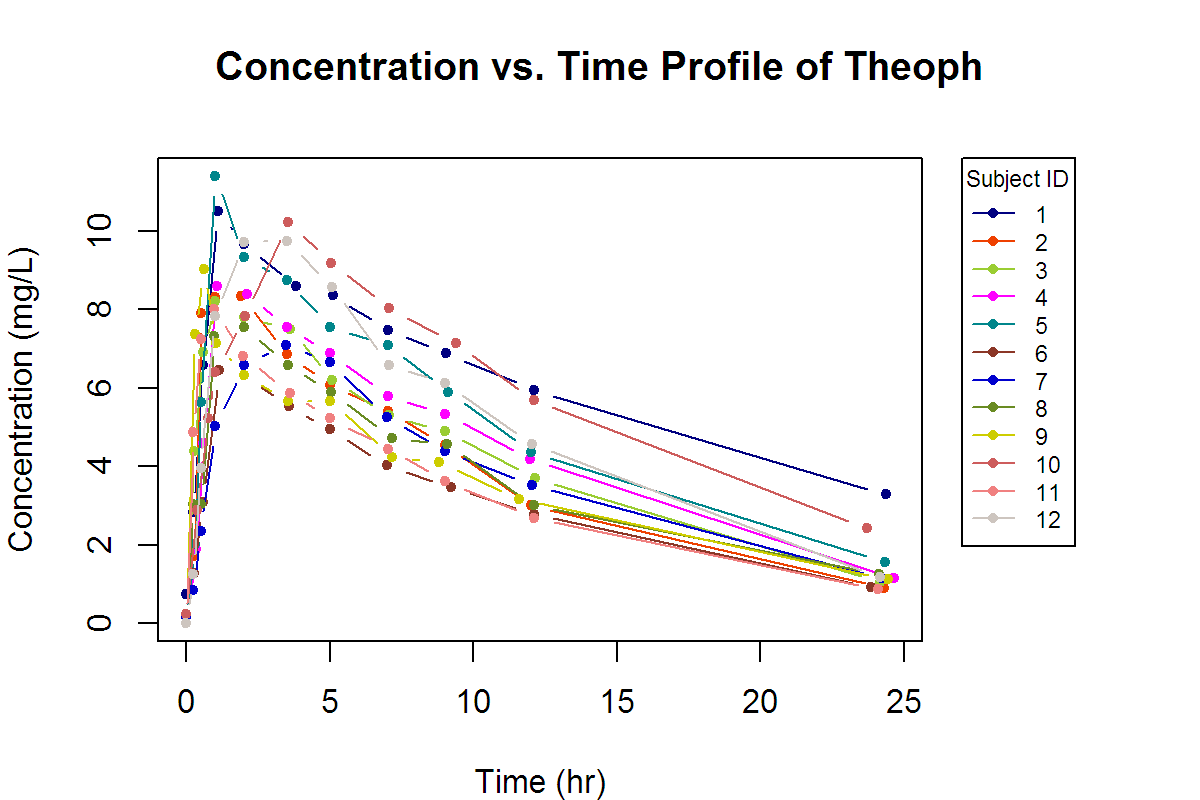
\includegraphics[width=1\linewidth]{Output/PK_Profile_Linear_Scale_for_Theoph} \caption{평균 약동학 파라메터와 그룹 농도-시간 그림 (선형)}\label{fig:unnamed-chunk-34}
\end{figure}

\begin{figure}
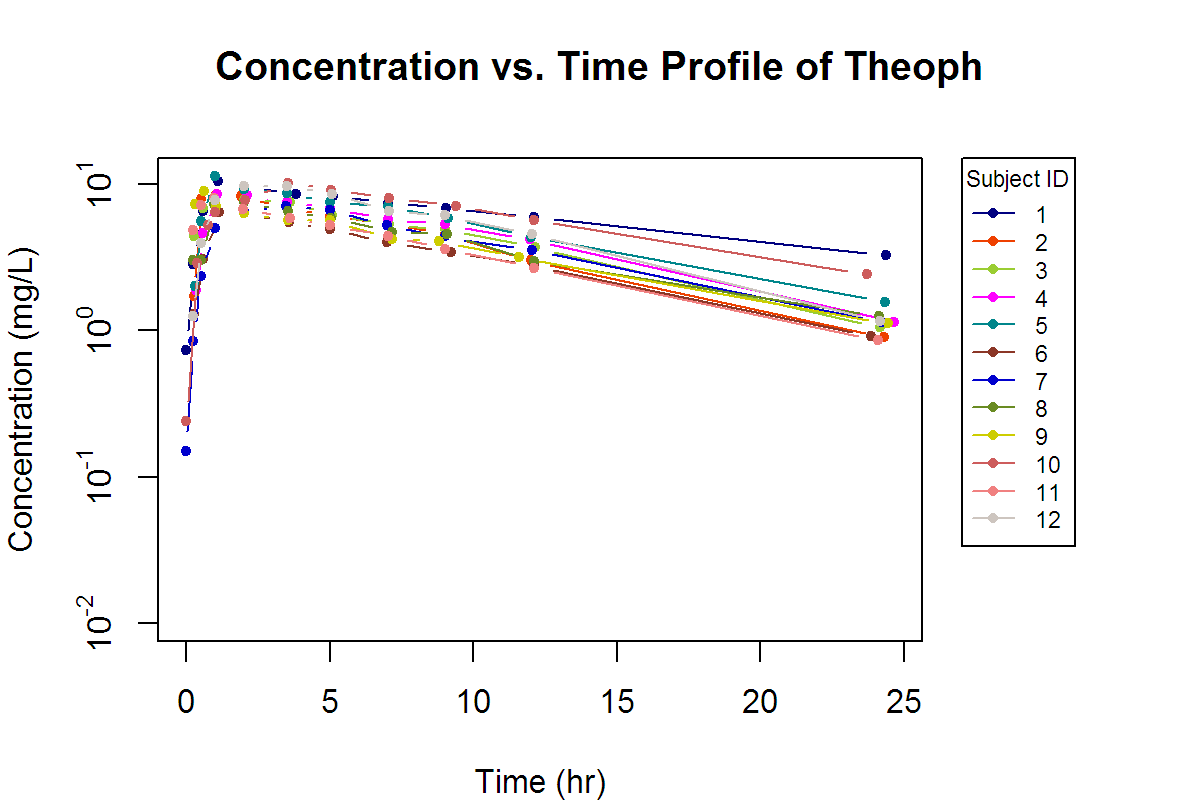
\includegraphics[width=1\linewidth]{Output/PK_Profile_Log_10_Scale_for_Theoph} \caption{평균 약동학 파라메터와 그룹 농도-시간 그림 (로그)}\label{fig:unnamed-chunk-35}
\end{figure}

\begin{figure}
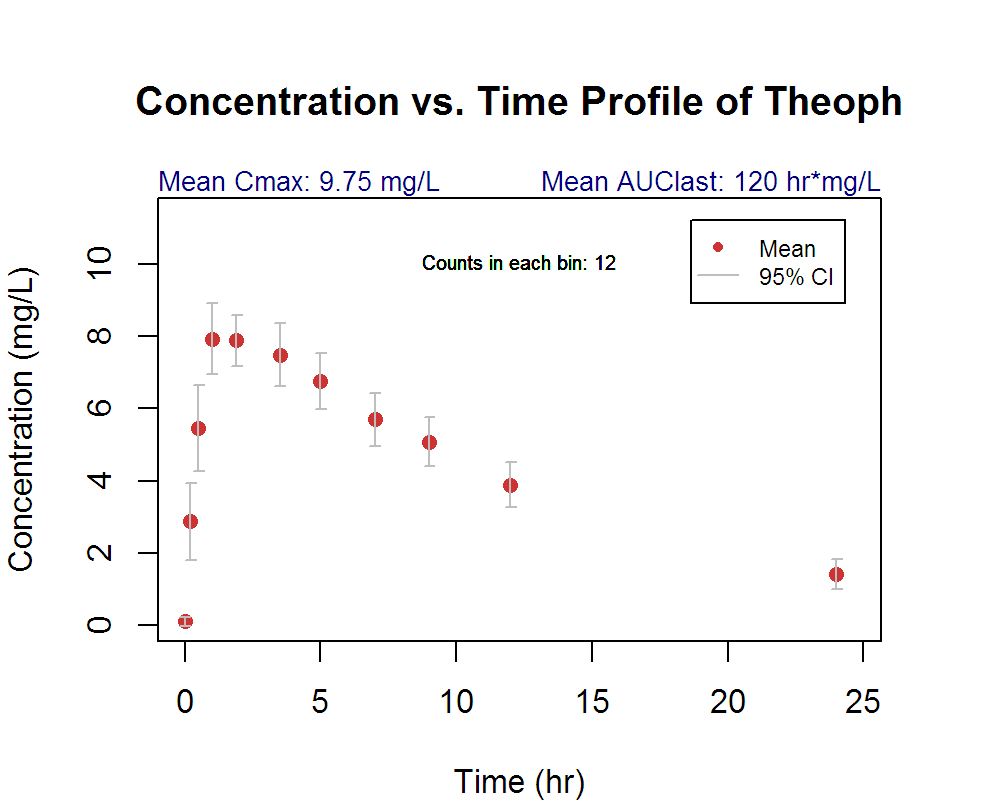
\includegraphics[width=1\linewidth]{Output/PK_Profile_with_CI_for_Theoph} \caption{평균 약동학 파라메터와 그룹 평균 농도-시간 그림 (로그)}\label{fig:unnamed-chunk-36}
\end{figure}

또한 개개인 별로 여러개의 그림이 담긴 두개의 PDF 파일이 생성되었습니다.

\begin{itemize}
\tightlist
\item
  ./Output//Individual PK Linear Scale for Theoph.pdf
\item
  ./Output//Individual PK Log 10 Scale for Theoph.pdf
\end{itemize}

\begin{figure}
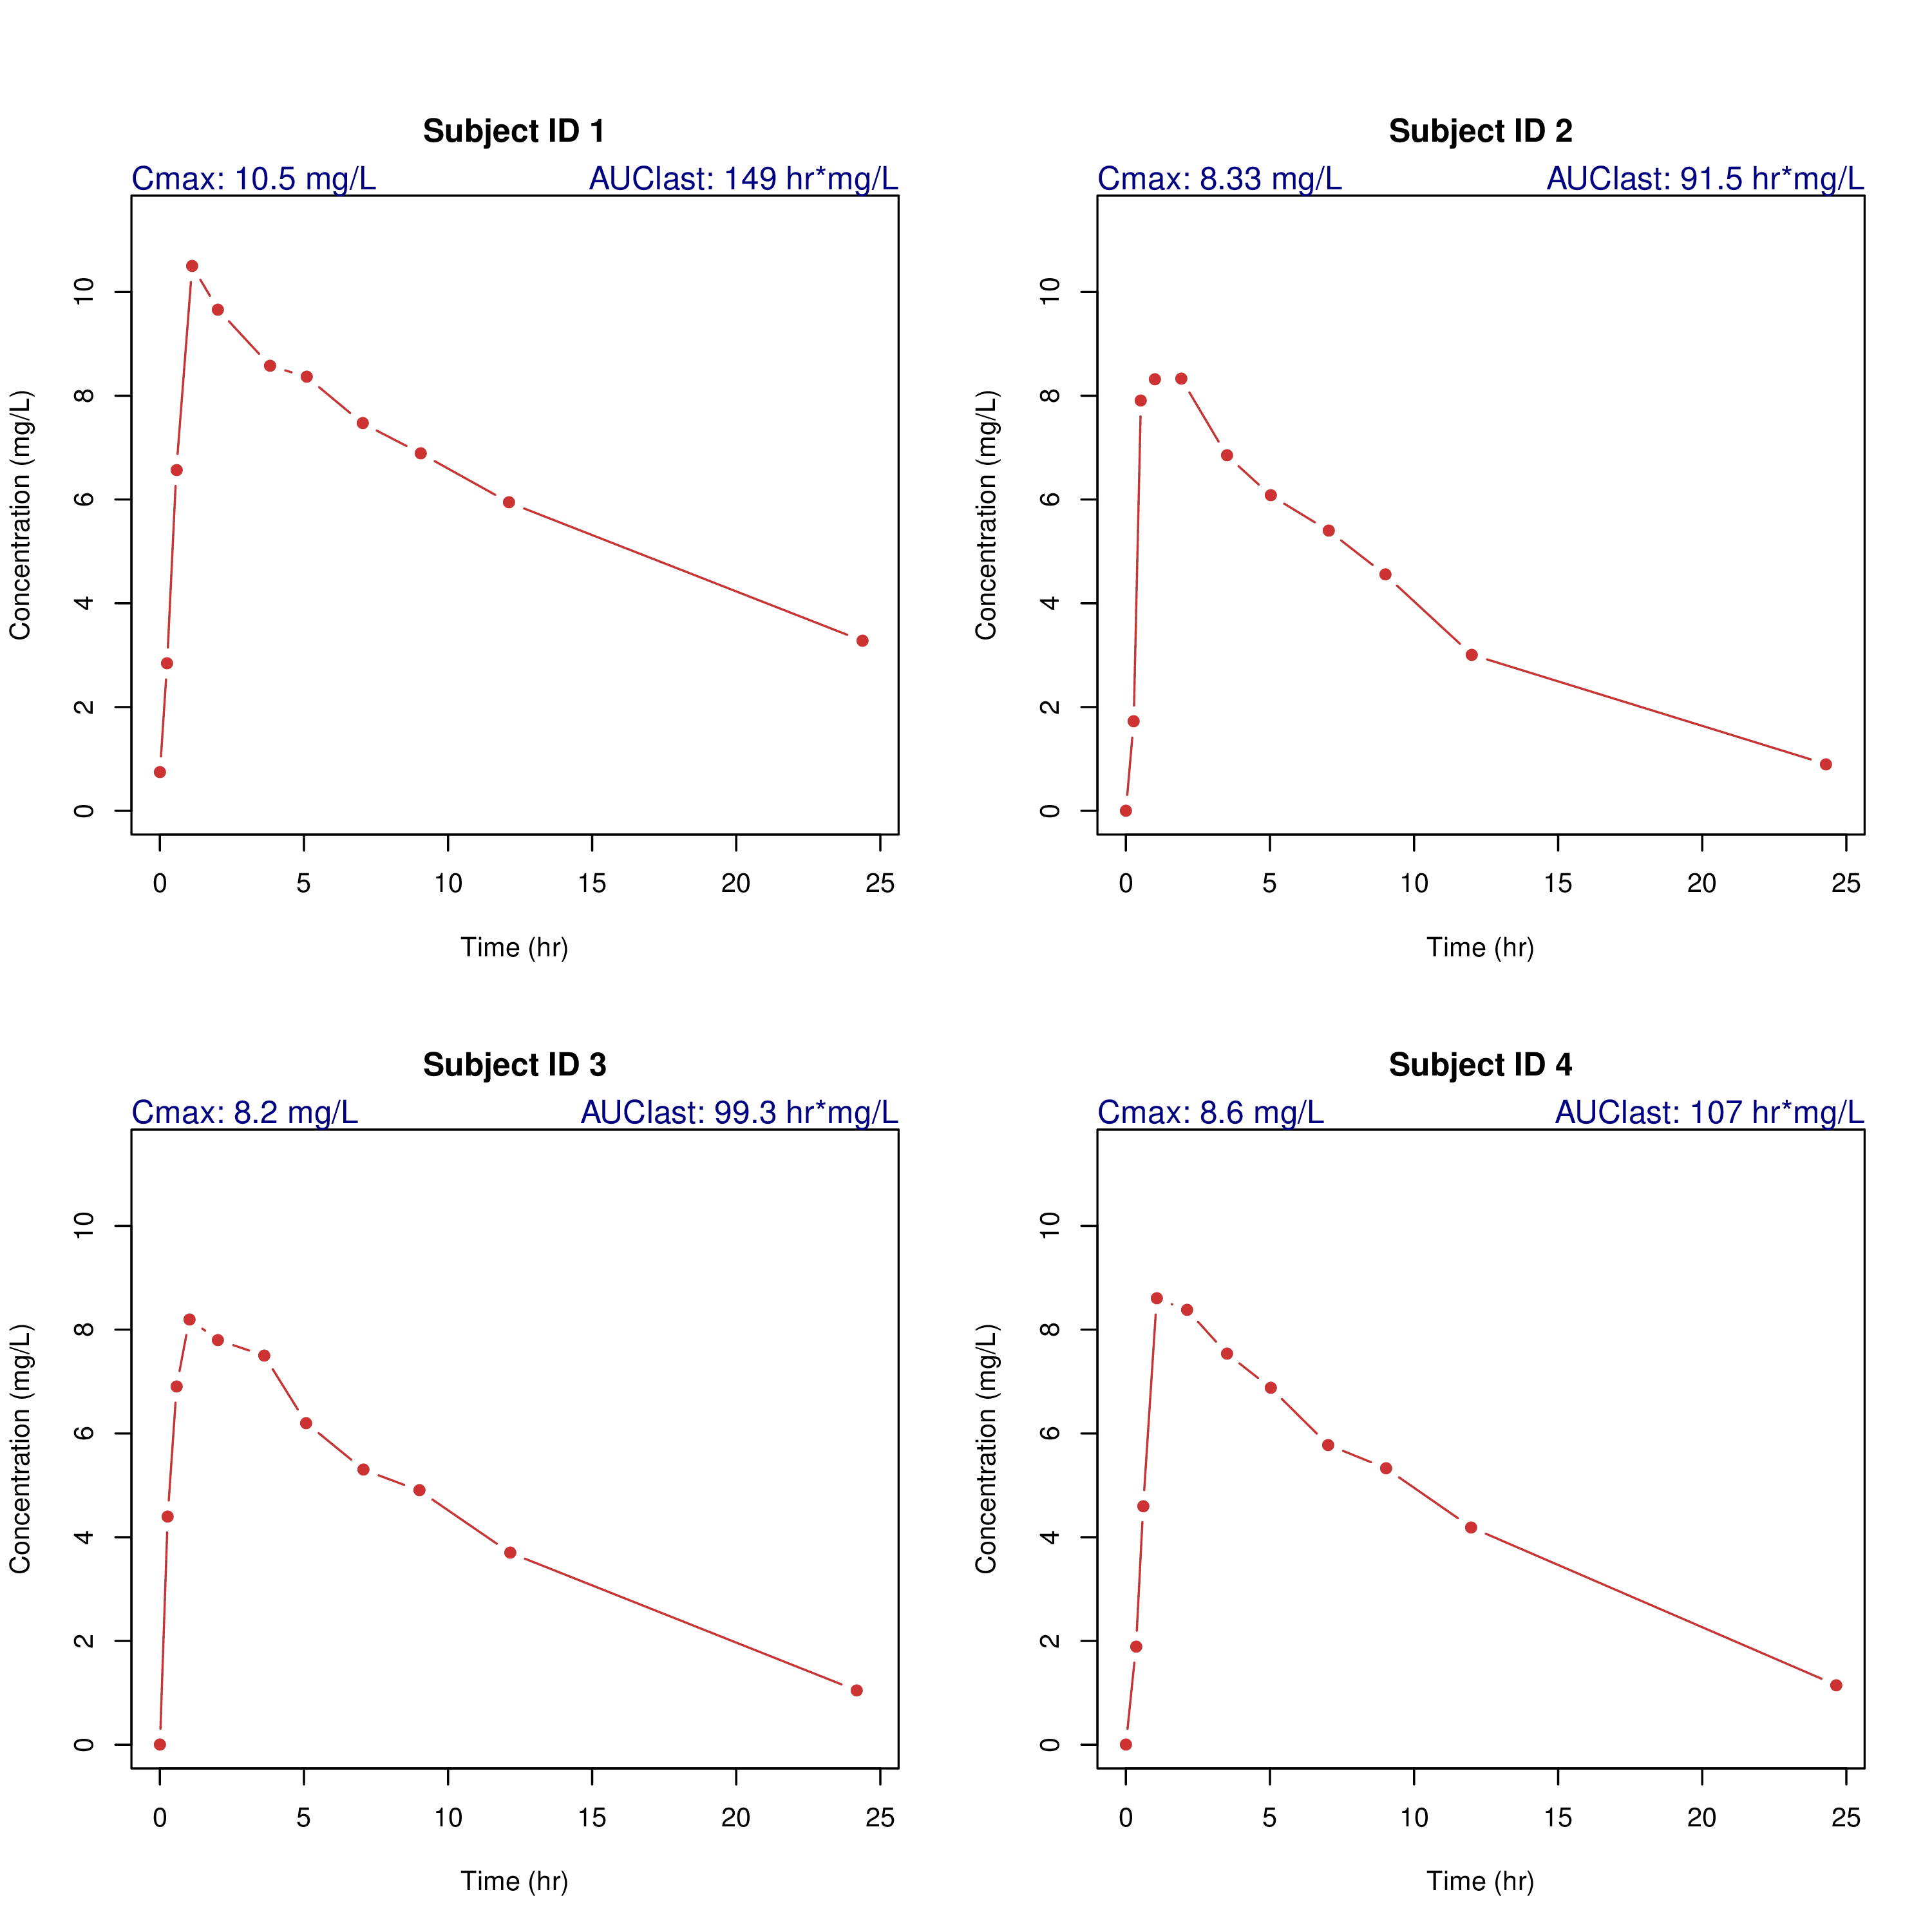
\includegraphics[width=1\linewidth]{Output/Individual_PK_Linear_Scale_for_Theoph00} \caption{약동학 파라메터와 함께 표시되는 농도-시간 그림 (선형)}\label{fig:unnamed-chunk-37}
\end{figure}

\begin{figure}
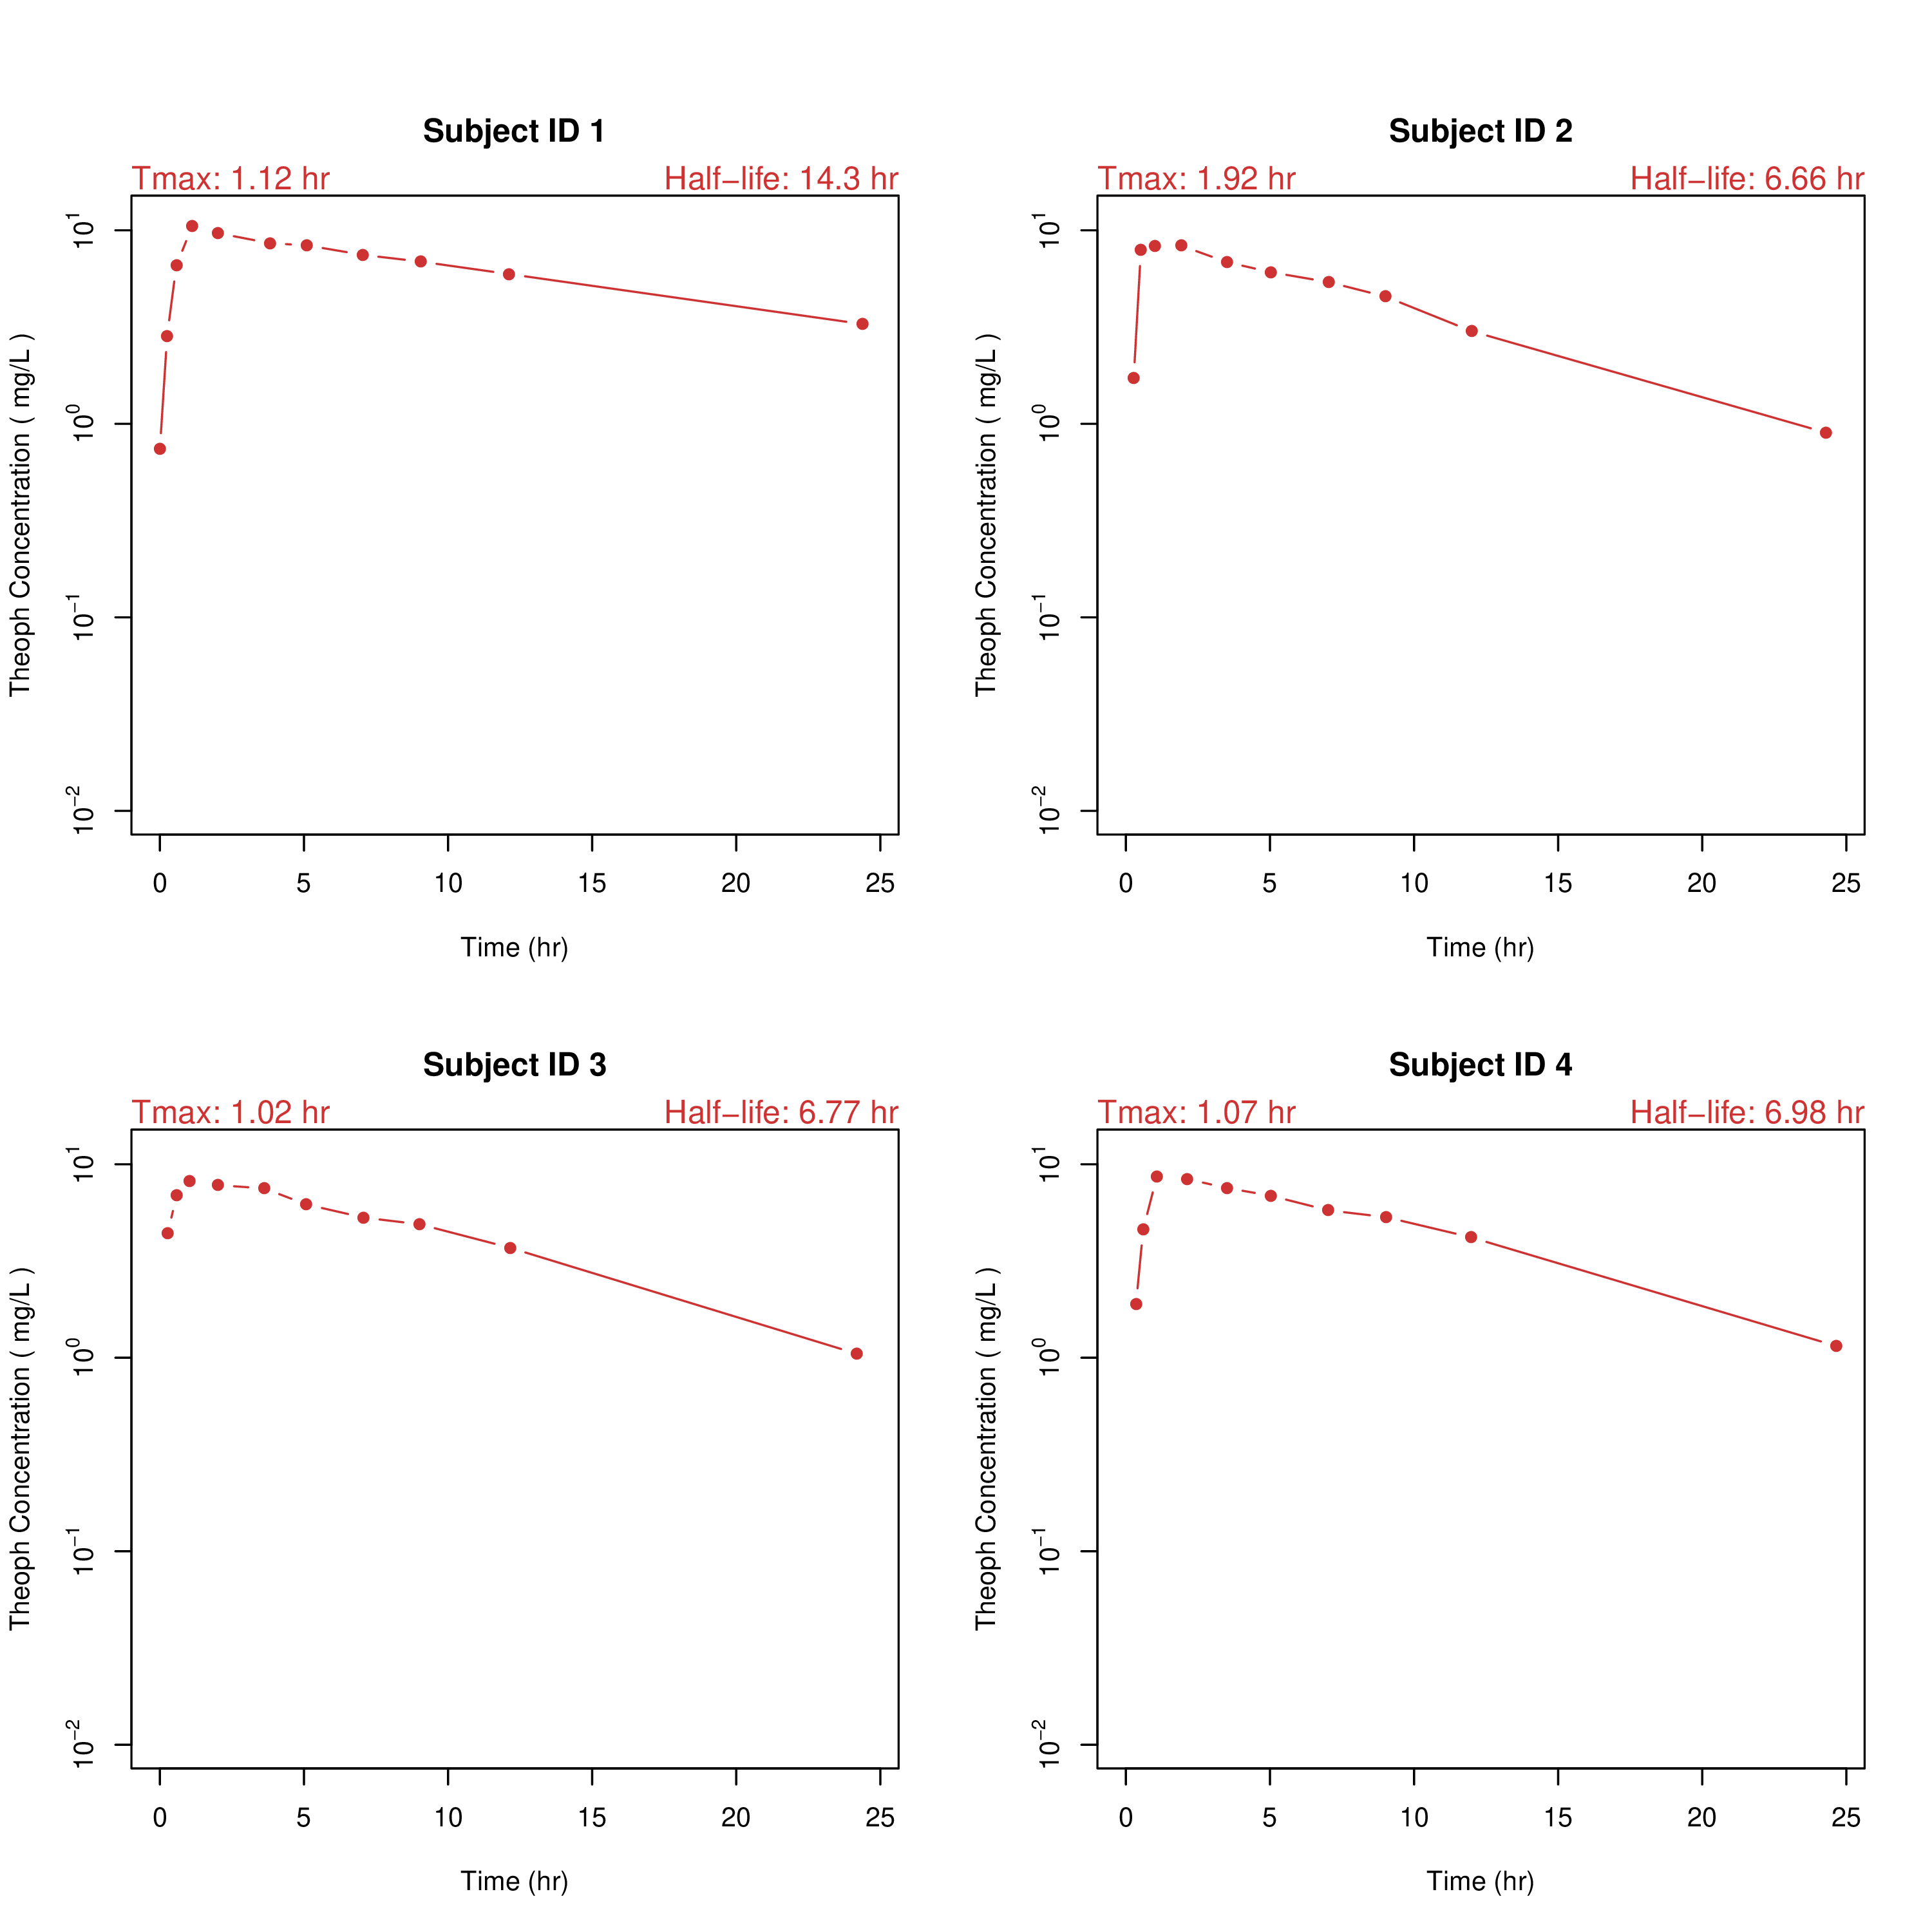
\includegraphics[width=1\linewidth]{Output/Individual_PK_Log_10_Scale_for_Theoph00} \caption{약동학 파라메터와 함께 표시되는 농도-시간 그림 (로그)}\label{fig:unnamed-chunk-38}
\end{figure}

\chapter{R을 사용한 약동학 시뮬레이션}\label{simulation}

\section{이 장에서는}\label{summary-simulation}

\section{시뮬레이션에 대하여}\label{-}

TBD

\texttt{wnl} 패키지가 CRAN에 올라와 있습니다.

\section{시뮬레이션 후 비구획분석}\label{--}

TBD

\section{앱을 통해 살펴보는 시뮬레이션}\label{---}

샤이니 앱을 통해서 시뮬레이션을 구현할 수 있습니다. Shinyapp: PK
Simulation - 1 Comp IV or Oral \url{https://asan.shinyapps.io/pk1c/}

\begin{Shaded}
\begin{Highlighting}[]
\NormalTok{knitr}\OperatorTok{::}\KeywordTok{include_app}\NormalTok{(}\StringTok{"https://asan.shinyapps.io/pk1c/"}\NormalTok{) }\CommentTok{#, height = "600px")}
\end{Highlighting}
\end{Shaded}

\begin{verbatim}
## Error in (function (url = NULL, file = "webshot.png", vwidth = 992, vheight = 744, : webshot.js returned failure value: 1
\end{verbatim}

\subsection{shiny 앱}\label{shiny-}

웹브라우저를 통해 간단히 비구획분석을 할 수 있는 앱을 개발하였습니다.

\begin{itemize}
\tightlist
\item
  Han, S. (2017) pkrshiny: Noncompartmental Analysis using pkr R package
  Shiny application. URL: \url{https://asan.shinyapps.io/pkrshiny}
\end{itemize}

그 외 약동학과 관련된 몇가지 shiny 앱도 참고하세요.

\begin{itemize}
\tightlist
\item
  Han, S. (2017) Pharmacokinetic Simulation of one-compartment Models.
  URL: \url{https://asan.shinyapps.io/pk1c/}
\item
  Han, S. (2017) caff: Monte Carlo Simulation of Caffeine Shiny
  application. URL: \url{https://asan.shinyapps.io/caff}
\item
  Han, S. (2016) vtdm: Vancomycin TDM Shiny application. URL:
  \url{https://asan.shinyapps.io/vtdm}
\end{itemize}

\chapter{통계처리}\label{statistics}

\section{이 장에서는}\label{stat-intro}

생물학적 동등성, 용량 비례성을 확인하는 통계 처리 방법을 알아보겠습니다.

\begin{Shaded}
\begin{Highlighting}[]
\KeywordTok{library}\NormalTok{(tidyverse)}
\KeywordTok{library}\NormalTok{(ncarbe)}
\KeywordTok{library}\NormalTok{(broom)}
\end{Highlighting}
\end{Shaded}

\section{기술통계량 구하기}\label{-}

앞서 \ref{noncompart}장에서 구한 \texttt{TheophNca}를 갖고 기술 통계량
(평균, 표준편차, 최소값, 최대값, skewness, kurtosis)을 구해보겠습니다.
\texttt{broom::tidy()} 함수를 사용하면 간단히 구할 수 있습니다. 다만
\texttt{NonCompart::tblNCA()} 후 \texttt{data.frame} 형태로 저장되어
입력으로 주어져야 합니다.

\begin{Shaded}
\begin{Highlighting}[]
\NormalTok{descStatTheophNca <-}\StringTok{ }\KeywordTok{tidy}\NormalTok{(}\KeywordTok{as.data.frame}\NormalTok{(TheophNca, }\DataTypeTok{stringsAsFactors =} \OtherTok{FALSE}\NormalTok{)) }\OperatorTok\StringTok{ }
\StringTok{  }\KeywordTok{select}\NormalTok{(column, n, mean, sd, min, max, skew, kurtosis)}

\NormalTok{knitr}\OperatorTok{::}\KeywordTok{kable}\NormalTok{(descStatTheophNca, }\DataTypeTok{digits =} \DecValTok{2}\NormalTok{)}
\end{Highlighting}
\end{Shaded}

\begin{tabular}{l|r|r|r|r|r|r|r}
\hline
column & n & mean & sd & min & max & skew & kurtosis\\
\hline
Subject* & 12 & 6.50 & 3.61 & 1.00 & 12.00 & 0.00 & -1.50\\
\hline
b0 & 12 & 2.39 & 0.25 & 2.03 & 2.82 & 0.13 & -1.38\\
\hline
CMAX & 12 & 8.76 & 1.47 & 6.44 & 11.40 & 0.21 & -1.19\\
\hline
CMAXD & 12 & 0.03 & 0.00 & 0.02 & 0.04 & 0.21 & -1.19\\
\hline
TMAX & 12 & 1.79 & 1.11 & 0.63 & 3.55 & 0.70 & -1.35\\
\hline
TLAG & 12 & 0.00 & 0.00 & 0.00 & 0.00 & NaN & NaN\\
\hline
CLST & 12 & 1.40 & 0.72 & 0.86 & 3.28 & 1.57 & 1.14\\
\hline
CLSTP & 12 & 1.40 & 0.72 & 0.86 & 3.28 & 1.58 & 1.19\\
\hline
TLST & 12 & 24.20 & 0.25 & 23.70 & 24.65 & -0.28 & -0.57\\
\hline
LAMZHL & 12 & 8.18 & 2.12 & 6.29 & 14.30 & 1.90 & 2.97\\
\hline
LAMZ & 12 & 0.09 & 0.02 & 0.05 & 0.11 & -0.92 & 0.40\\
\hline
LAMZLL & 12 & 7.49 & 2.40 & 2.03 & 9.38 & -1.20 & -0.03\\
\hline
LAMZUL & 12 & 24.20 & 0.25 & 23.70 & 24.65 & -0.28 & -0.57\\
\hline
LAMZNPT & 12 & 3.83 & 1.34 & 3.00 & 7.00 & 1.32 & 0.28\\
\hline
CORRXY & 12 & -1.00 & 0.00 & -1.00 & -1.00 & 2.20 & 3.87\\
\hline
R2 & 12 & 1.00 & 0.00 & 0.99 & 1.00 & -2.20 & 3.87\\
\hline
R2ADJ & 12 & 1.00 & 0.00 & 0.99 & 1.00 & -2.05 & 3.39\\
\hline
AUCLST & 12 & 103.81 & 23.65 & 73.78 & 148.92 & 0.56 & -1.12\\
\hline
AUCALL & 12 & 103.81 & 23.65 & 73.78 & 148.92 & 0.56 & -1.12\\
\hline
AUCIFO & 12 & 122.19 & 38.13 & 84.25 & 216.61 & 1.25 & 0.51\\
\hline
AUCIFOD & 12 & 0.38 & 0.12 & 0.26 & 0.68 & 1.25 & 0.51\\
\hline
AUCIFP & 12 & 122.18 & 38.11 & 84.50 & 216.61 & 1.26 & 0.52\\
\hline
AUCIFPD & 12 & 0.38 & 0.12 & 0.26 & 0.68 & 1.26 & 0.52\\
\hline
AUCPEO & 12 & 13.54 & 6.35 & 8.13 & 31.25 & 1.71 & 2.19\\
\hline
AUCPEP & 12 & 13.54 & 6.34 & 8.16 & 31.25 & 1.72 & 2.23\\
\hline
AUMCLST & 12 & 883.06 & 262.98 & 609.15 & 1459.07 & 0.92 & -0.42\\
\hline
AUMCIFO & 12 & 1590.30 & 1006.57 & 928.56 & 4505.53 & 2.00 & 2.96\\
\hline
AUMCIFP & 12 & 1589.85 & 1006.06 & 928.49 & 4505.67 & 2.01 & 2.97\\
\hline
AUMCPEO & 12 & 38.72 & 11.10 & 26.50 & 67.62 & 1.29 & 1.10\\
\hline
AUMCPEP & 12 & 38.72 & 11.07 & 26.59 & 67.62 & 1.30 & 1.14\\
\hline
VZFO & 12 & 31.93 & 6.47 & 22.22 & 43.26 & 0.20 & -1.40\\
\hline
VZFP & 12 & 31.92 & 6.46 & 22.22 & 43.14 & 0.19 & -1.41\\
\hline
CLFO & 12 & 2.81 & 0.68 & 1.48 & 3.80 & -0.45 & -0.93\\
\hline
CLFP & 12 & 2.81 & 0.68 & 1.48 & 3.79 & -0.46 & -0.93\\
\hline
MRTEVLST & 12 & 8.41 & 0.59 & 7.71 & 9.80 & 0.99 & 0.12\\
\hline
MRTEVIFO & 12 & 12.29 & 2.96 & 9.98 & 20.80 & 1.90 & 2.83\\
\hline
MRTEVIFP & 12 & 12.29 & 2.95 & 9.95 & 20.80 & 1.91 & 2.84\\
\hline
\end{tabular}

\section{생물학적 동등성}\label{bioequivalence}

생물학적 동등성을 위한 가장 간단한 방법은 \texttt{ncarbe} 패키지(Bae and
Han \protect\hyperlink{ref-R-ncarbe}{2018})를 쓰는 것입니다.

\begin{Shaded}
\begin{Highlighting}[]
\KeywordTok{install.packages}\NormalTok{(}\StringTok{'devtools'}\NormalTok{)}
\NormalTok{devtools}\OperatorTok{::}\KeywordTok{install_github}\NormalTok{(}\StringTok{'asancpt/ncarbe'}\NormalTok{)}
\end{Highlighting}
\end{Shaded}

Chow와 Liu의 책의 내용을 충실히 반영하였습니다. (Chow
\protect\hyperlink{ref-chow2009design}{2009}) 생물학적 동등성을 위한
수학 식은 다음과 같습니다. \eqref{eq:be}

\[
\begin{align}
  0.8 < 90\%\ CI\ of\ \frac{GM(AUC_{last, test})}{GM(AUC_{last, ref})} < 1.25 \\
  0.8 < 90\%\ CI\ of\ \frac{GM(AUC_{last, test})}{GM(AUC_{last, ref})} < 1.25 \label{eq:be}
\end{align}
\]

현재로서는 2x2 디자인의 간단한 임상시험 디자인만을 지원하고 있습니다.
(그림 \ref{fig:twobytwo}) 핵심이 되는 함수는 \texttt{beNCA()} 입니다.

\begin{Shaded}
\begin{Highlighting}[]
\NormalTok{knitr}\OperatorTok{::}\KeywordTok{include_graphics}\NormalTok{(}\StringTok{'assets/twobytwo.jpg'}\NormalTok{)}
\end{Highlighting}
\end{Shaded}

\begin{figure}
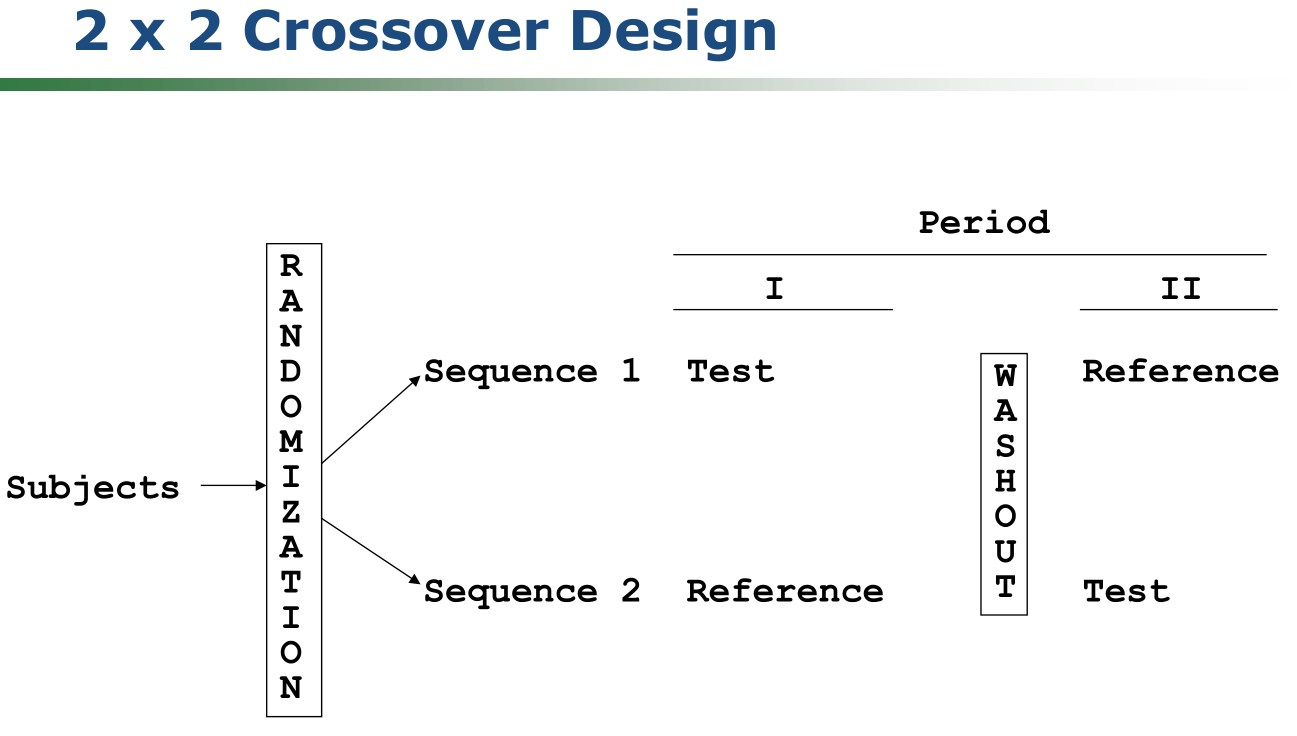
\includegraphics[width=1\linewidth]{assets/twobytwo} \caption{전형적인 2x2 설계}\label{fig:twobytwo}
\end{figure}

\begin{verbatim}
## function (concData, SUBJ = "SUBJ", GRP = "GRP", PRD = "PRD", 
##     TRT = "TRT", method = "kbe", ...) 
## NULL
\end{verbatim}

다음과 같은 함수 인자를 설정해 주면 됩니다.

\begin{itemize}
\tightlist
\item
  SUBJ: Subject ID, any data type
\item
  GRP: column name in which information of ``RT'' or ``TR'' exists.
\item
  PRD: column name in which information of 1 or 2 exists.
\item
  TRT: column name in which information of ``R'' or ``T'' exists.
\item
  method: \texttt{kbe} by authors or \texttt{nlme} package uploaded on
  CRAN
\end{itemize}

ncarbe 패키지 내에 있는 자료를 사용할 것입니다. (Table
\ref{tab:beconcdata})

\begin{Shaded}
\begin{Highlighting}[]
\NormalTok{file <-}\StringTok{ }\KeywordTok{system.file}\NormalTok{(}\StringTok{'example'}\NormalTok{, }\StringTok{'beConc.csv'}\NormalTok{, }\DataTypeTok{package =} \StringTok{'ncarbe'}\NormalTok{)}
\NormalTok{concData <-}\StringTok{ }\KeywordTok{read_csv}\NormalTok{(file)}
\end{Highlighting}
\end{Shaded}

\begin{table}

\caption{\label{tab:beconcdata}A example dataset for the bioequivalence test.}
\centering
\begin{tabular}[t]{r|l|r|l|r|r|r}
\hline
SUBJ & GRP & PRD & TRT & nTIME & TIME & CONC\\
\hline
1 & RT & 1 & R & 0.00 & 0.02 & 63.42\\
\hline
1 & RT & 1 & R & 0.25 & 0.24 & 432.76\\
\hline
1 & RT & 1 & R & 0.50 & 0.51 & 622.88\\
\hline
1 & RT & 1 & R & 0.75 & 0.80 & 809.93\\
\hline
1 & RT & 1 & R & 1.00 & 1.02 & 824.34\\
\hline
1 & RT & 1 & R & 2.00 & 2.04 & 602.22\\
\hline
1 & RT & 1 & R & 3.00 & 2.96 & 512.28\\
\hline
1 & RT & 1 & R & 4.00 & 3.99 & 421.99\\
\hline
1 & RT & 1 & R & 6.00 & 6.04 & 302.73\\
\hline
1 & RT & 1 & R & 8.00 & 8.04 & 181.60\\
\hline
\end{tabular}
\end{table}

\begin{Shaded}
\begin{Highlighting}[]
\KeywordTok{beNCA}\NormalTok{(concData)}
\end{Highlighting}
\end{Shaded}

\begin{verbatim}
## 
## 
## [AUClast]
## 
## $`Analysis of Variance`
##                       SS DF         MS        F          p
## SUBJECT        2.8102897 35 0.08029399 1.972327 0.02517703
## GROUP          0.2811516  1 0.28115157 3.779609 0.06019307
## SUBJECT(GROUP) 2.5291381 34 0.07438642 1.827214 0.04166286
## PERIOD         0.2887407  1 0.28874073 7.092573 0.01174249
## DRUG           0.1186721  1 0.11867210 2.915039 0.09687516
## ERROR          1.3841500 34 0.04071029       NA         NA
## TOTAL          4.5500268 71         NA       NA         NA
## 
## $`Between and Within Subject Variability`
##                                 Between Subject Within Subject
## Variance Estimate                    0.01683806     0.04071029
## Coefficient of Variation, CV(%)     13.03097098    20.38389491
## 
## $`Least Square Means`
##                 Reference Drug Test Drug
## Geometric Means       5047.026  4648.063
## 
## $`90% Confidence Interval`
##                  Lower Limit Point Estimate Upper Limit
## 90% CI for Ratio   0.8488229       0.920951   0.9992081
## 
## $`Sample Size`
##                       True Ratio=1 True Ratio=Point Estimate
## 80% Power Sample Size            8                        14
## 
## 
## 
## [Cmax]
## 
## $`Analysis of Variance`
##                        SS DF         MS         F         p
## SUBJECT        2.85581816 35 0.08159480 0.9694346 0.5367126
## GROUP          0.08840271  1 0.08840271 1.0861008 0.3046908
## SUBJECT(GROUP) 2.76741545 34 0.08139457 0.9670557 0.5386164
## PERIOD         0.04931289  1 0.04931289 0.5858905 0.4492937
## DRUG           0.10908566  1 0.10908566 1.2960558 0.2628934
## ERROR          2.86169200 34 0.08416741        NA        NA
## TOTAL          5.85528790 71         NA        NA        NA
## 
## $`Between and Within Subject Variability`
##                                 Between Subject Within Subject
## Variance Estimate                   -0.00138642     0.08416741
## Coefficient of Variation, CV(%)             NaN    29.63291938
## 
## $`Least Square Means`
##                 Reference Drug Test Drug
## Geometric Means       791.1619     731.1
## 
## $`90% Confidence Interval`
##                  Lower Limit Point Estimate Upper Limit
## 90% CI for Ratio   0.8218317       0.924084    1.039059
## 
## $`Sample Size`
##                       True Ratio=1 True Ratio=Point Estimate
## 80% Power Sample Size           16                        26
## 
## 
## 
## [Tmax]
## 
## $`Wilcoxon Signed-Rank Test`
##   p-value 
## 0.3059991 
## 
## $`Hodges-Lehmann Estimate`
##                            Lower Limit Point Estimate Upper Limit
## 90% Confidence Interval       -0.10000         0.0300       0.405
## 90% Confidence Interval(%)    92.18517       102.3444     131.650
\end{verbatim}

배균섭 교수님의 강의 자료에서 가져왔습니다.

\begin{Shaded}
\begin{Highlighting}[]
\NormalTok{knitr}\OperatorTok{::}\KeywordTok{include_graphics}\NormalTok{(}\StringTok{'assets/fixed-random.jpg'}\NormalTok{)}
\end{Highlighting}
\end{Shaded}

\begin{figure}
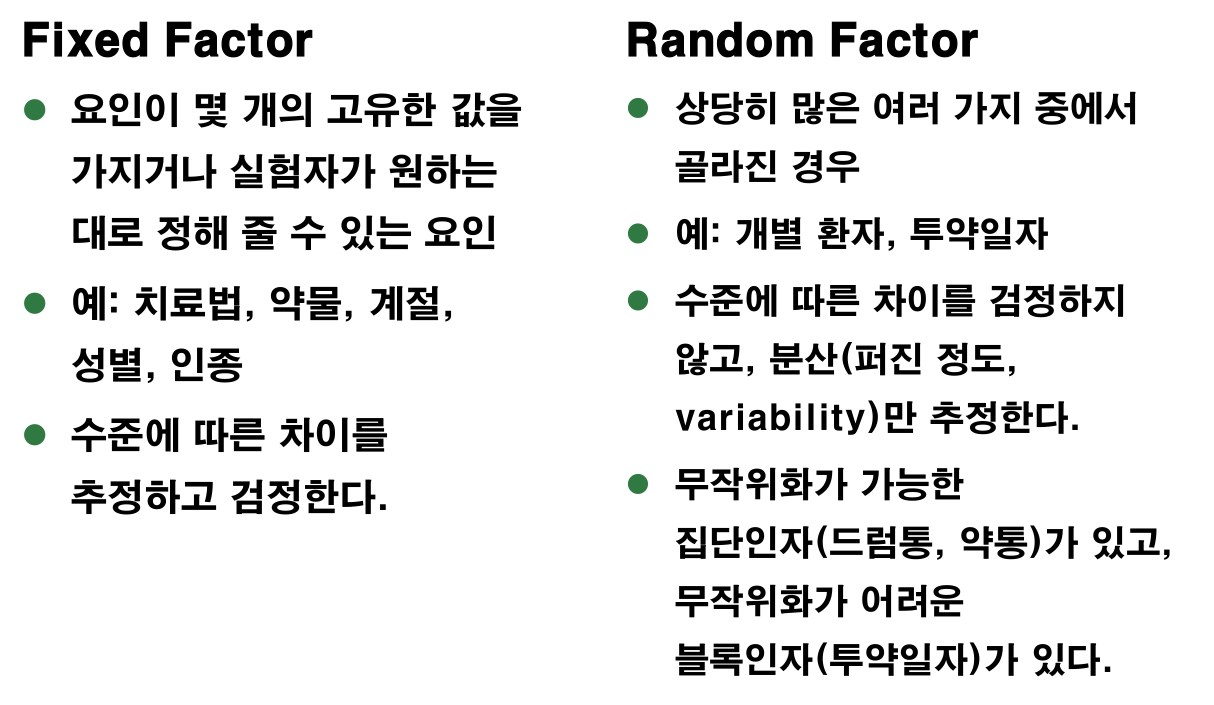
\includegraphics[width=1\linewidth]{assets/fixed-random} \caption{모수 인자와 변량 인자의 비교}\label{fig:fixedrandom}
\end{figure}

\section{Dose Proportionality}\label{dp}

DP 처리.

16명의 C\textsubscript{max}와 AUC\textsubscript{last}가 나온 표입니다.
Table \ref{tab:sad-pk}

\begin{Shaded}
\begin{Highlighting}[]
\CommentTok{# setup ----}

\KeywordTok{library}\NormalTok{(readxl)}
\KeywordTok{library}\NormalTok{(tidyverse)}
\KeywordTok{library}\NormalTok{(broom)}

\NormalTok{dp_data <-}\StringTok{ }\CommentTok{# Virtual data from 4 dose groups (N=16)}
\StringTok{'Dose,Subject,Cmax,AUClast}
\StringTok{50,101,860,2000}
\StringTok{50,102,510,2300}
\StringTok{50,103,620,2900}
\StringTok{50,104,540,2400}
\StringTok{100,201,1550,6600}
\StringTok{100,202,1440,7400}
\StringTok{100,203,2000,7300}
\StringTok{100,204,1600,7000}
\StringTok{200,301,4100,20400}
\StringTok{200,302,2800,9500}
\StringTok{200,303,3200,8000}
\StringTok{200,304,2550,7070}
\StringTok{400,401,4800,22000}
\StringTok{400,402,5700,23000}
\StringTok{400,403,5800,26700}
\StringTok{400,404,5760,28884'}

\NormalTok{sad_indi_pk <-}\StringTok{ }\KeywordTok{read_csv}\NormalTok{(dp_data)}
\NormalTok{knitr}\OperatorTok{::}\KeywordTok{kable}\NormalTok{(sad_indi_pk, }\DataTypeTok{caption =} \StringTok{'16명의 C~max~, AUC~last~'}\NormalTok{)}
\end{Highlighting}
\end{Shaded}

\begin{table}

\caption{\label{tab:sad-pk}16명의 C~max~, AUC~last~}
\centering
\begin{tabular}[t]{r|r|r|r}
\hline
Dose & Subject & Cmax & AUClast\\
\hline
50 & 101 & 860 & 2000\\
\hline
50 & 102 & 510 & 2300\\
\hline
50 & 103 & 620 & 2900\\
\hline
50 & 104 & 540 & 2400\\
\hline
100 & 201 & 1550 & 6600\\
\hline
100 & 202 & 1440 & 7400\\
\hline
100 & 203 & 2000 & 7300\\
\hline
100 & 204 & 1600 & 7000\\
\hline
200 & 301 & 4100 & 20400\\
\hline
200 & 302 & 2800 & 9500\\
\hline
200 & 303 & 3200 & 8000\\
\hline
200 & 304 & 2550 & 7070\\
\hline
400 & 401 & 4800 & 22000\\
\hline
400 & 402 & 5700 & 23000\\
\hline
400 & 403 & 5800 & 26700\\
\hline
400 & 404 & 5760 & 28884\\
\hline
\end{tabular}
\end{table}

그림을 살펴보겠습니다.

\begin{Shaded}
\begin{Highlighting}[]
\NormalTok{sad_indi_pk_log <-}\StringTok{ }\NormalTok{sad_indi_pk }\OperatorTok\StringTok{ }\KeywordTok{mutate_all}\NormalTok{(log)}

\NormalTok{figA <-}\StringTok{ }\KeywordTok{ggplot}\NormalTok{(sad_indi_pk_log, }\KeywordTok{aes}\NormalTok{(}\DataTypeTok{x=}\NormalTok{Dose, }\DataTypeTok{y=}\NormalTok{Cmax)) }\OperatorTok{+}
\StringTok{  }\KeywordTok{geom_smooth}\NormalTok{(}\DataTypeTok{method =} \StringTok{'lm'}\NormalTok{)}\OperatorTok{+}
\StringTok{  }\KeywordTok{geom_boxplot}\NormalTok{(}\KeywordTok{aes}\NormalTok{(}\DataTypeTok{group =}\NormalTok{ Dose), }
               \DataTypeTok{size =} \DecValTok{1}\NormalTok{, }
               \DataTypeTok{outlier.colour =} \StringTok{"red"}\NormalTok{, }
               \DataTypeTok{outlier.shape =} \DecValTok{1}\NormalTok{, }
               \DataTypeTok{outlier.size =} \DecValTok{3}\NormalTok{) }\OperatorTok{+}
\StringTok{  }\KeywordTok{theme_bw}\NormalTok{() }\OperatorTok{+}
\StringTok{  }\KeywordTok{scale_x_continuous}\NormalTok{(}\DataTypeTok{breaks =} \KeywordTok{c}\NormalTok{(}\DecValTok{50}\NormalTok{, }\DecValTok{100}\NormalTok{, }\DecValTok{200}\NormalTok{, }\DecValTok{400}\NormalTok{)) }\OperatorTok{+}
\StringTok{  }\KeywordTok{labs}\NormalTok{(}\DataTypeTok{x =} \StringTok{'Dose (mg)'}\NormalTok{, }\DataTypeTok{y =} \KeywordTok{expression}\NormalTok{(}\StringTok{'C'}\NormalTok{[max]}\OperatorTok{*}\StringTok{' (ng/mL)'}\NormalTok{),}
       \DataTypeTok{title =} \KeywordTok{expression}\NormalTok{(}\StringTok{'C'}\NormalTok{[max]))}
\NormalTok{figA}
\end{Highlighting}
\end{Shaded}

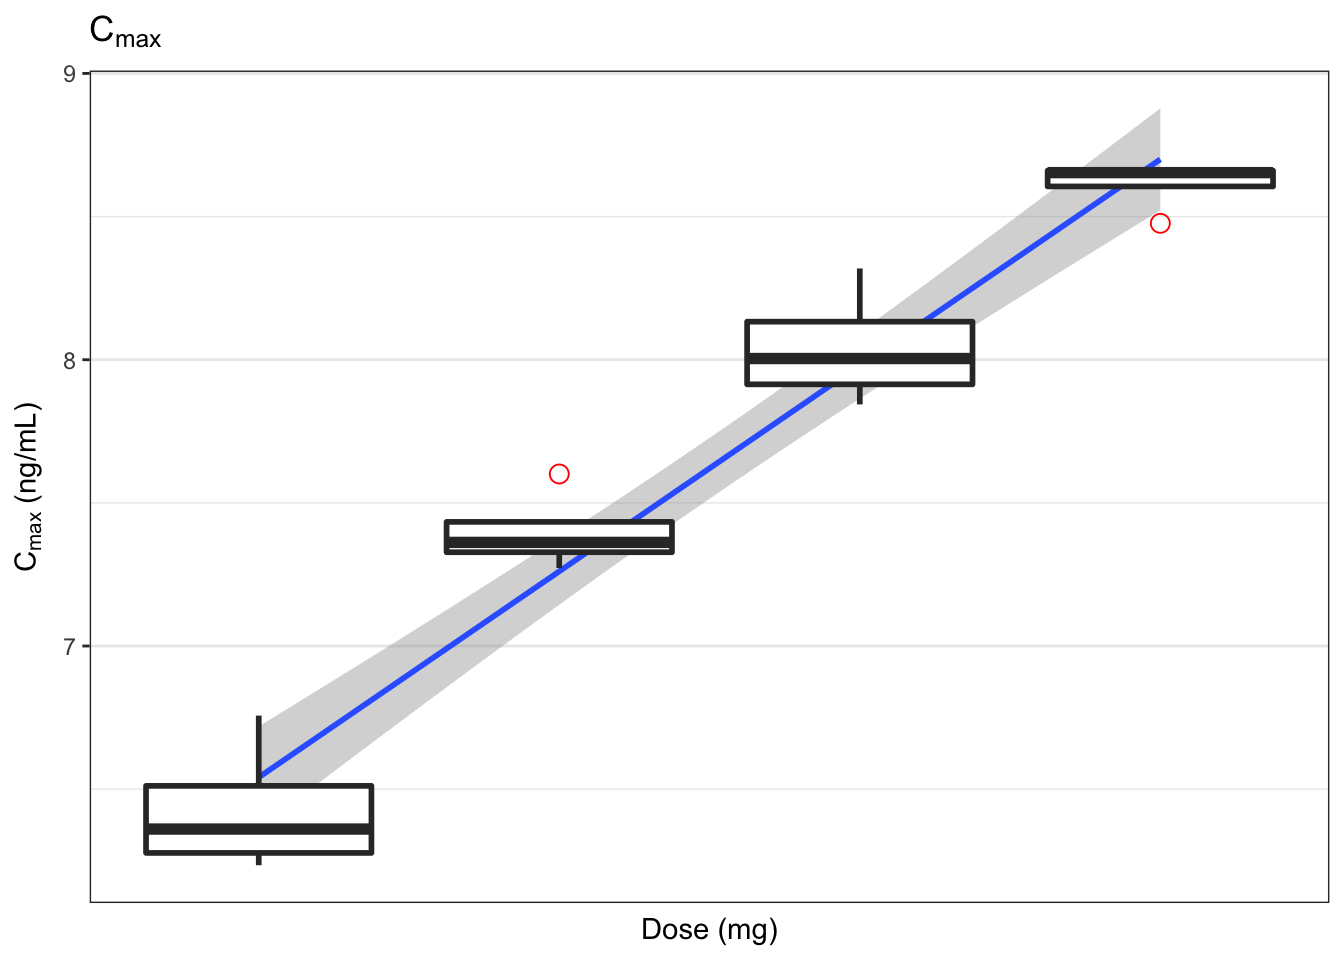
\includegraphics[width=1\linewidth]{book-ncar_files/figure-latex/sad-indi-pk-log-1}

\begin{Shaded}
\begin{Highlighting}[]
\NormalTok{figB <-}\StringTok{ }\KeywordTok{ggplot}\NormalTok{(sad_indi_pk_log, }\KeywordTok{aes}\NormalTok{(}\DataTypeTok{x=}\NormalTok{Dose, }\DataTypeTok{y=}\NormalTok{AUClast)) }\OperatorTok{+}
\StringTok{  }\KeywordTok{geom_smooth}\NormalTok{(}\DataTypeTok{method =} \StringTok{'lm'}\NormalTok{)}\OperatorTok{+}
\StringTok{  }\KeywordTok{geom_boxplot}\NormalTok{(}\KeywordTok{aes}\NormalTok{(}\DataTypeTok{group =}\NormalTok{ Dose), }
               \DataTypeTok{size =} \DecValTok{1}\NormalTok{, }
               \DataTypeTok{outlier.colour =} \StringTok{"red"}\NormalTok{, }
               \DataTypeTok{outlier.shape =} \DecValTok{1}\NormalTok{, }
               \DataTypeTok{outlier.size =} \DecValTok{3}\NormalTok{) }\OperatorTok{+}
\StringTok{  }\KeywordTok{theme_bw}\NormalTok{() }\OperatorTok{+}
\StringTok{  }\KeywordTok{scale_x_continuous}\NormalTok{(}\DataTypeTok{breaks =} \KeywordTok{c}\NormalTok{(}\DecValTok{50}\NormalTok{, }\DecValTok{100}\NormalTok{, }\DecValTok{200}\NormalTok{, }\DecValTok{400}\NormalTok{)) }\OperatorTok{+}
\StringTok{  }\KeywordTok{labs}\NormalTok{(}\DataTypeTok{x =} \StringTok{'Dose (mg)'}\NormalTok{, }\DataTypeTok{y =} \KeywordTok{expression}\NormalTok{(}\StringTok{'AUC'}\NormalTok{[(}\DecValTok{0}\OperatorTok{-}\NormalTok{last)]}\OperatorTok{*}\StringTok{' (ng·hr/mL)'}\NormalTok{),}
       \DataTypeTok{title =} \KeywordTok{expression}\NormalTok{(}\StringTok{'AUC'}\NormalTok{[(}\DecValTok{0}\OperatorTok{-}\NormalTok{last)]))}
\NormalTok{figB}
\end{Highlighting}
\end{Shaded}

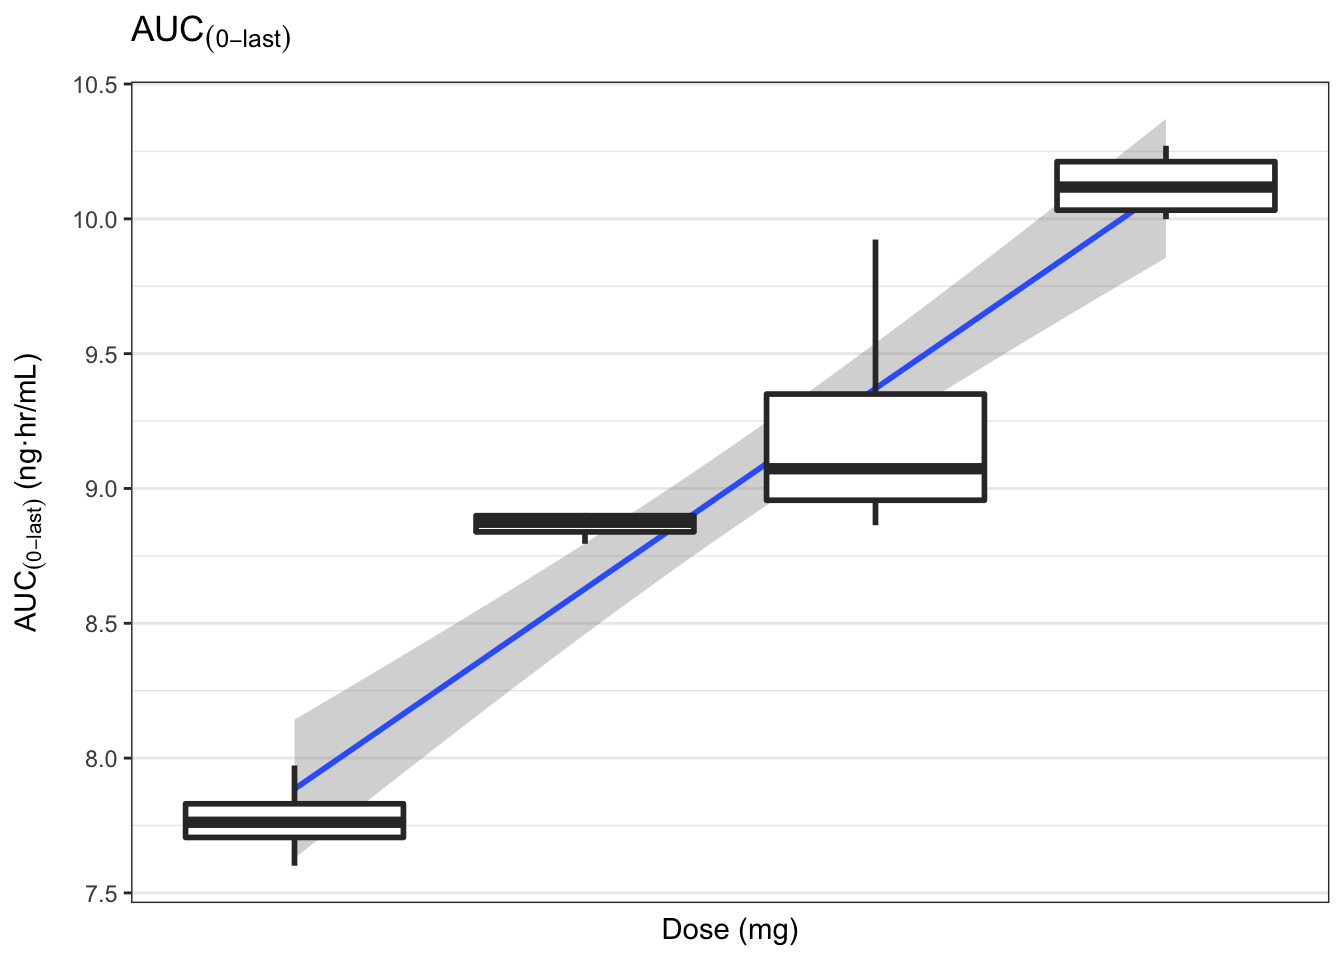
\includegraphics[width=1\linewidth]{book-ncar_files/figure-latex/sad-indi-pk-log-2}

lm() 함수를 써서 구할 수 있습니다.

\begin{Shaded}
\begin{Highlighting}[]
\NormalTok{calc_dp <-}\StringTok{ }\ControlFlowTok{function}\NormalTok{(param, fit) \{}
  \KeywordTok{bind_cols}\NormalTok{(fit }\OperatorTok\StringTok{ }\NormalTok{summary }\OperatorTok\StringTok{ }\NormalTok{tidy }\OperatorTok\StringTok{ }\KeywordTok{filter}\NormalTok{(term }\OperatorTok{==}\StringTok{ 'Dose'}\NormalTok{), }
\NormalTok{            fit }\OperatorTok\StringTok{ }\KeywordTok{confint}\NormalTok{(}\DataTypeTok{level =} \FloatTok{0.95}\NormalTok{) }\OperatorTok\StringTok{ }\NormalTok{tidy }\OperatorTok\StringTok{ }\KeywordTok{filter}\NormalTok{(.rownames }\OperatorTok{==}\StringTok{ 'Dose'}\NormalTok{), }
\NormalTok{            fit }\OperatorTok\StringTok{ }\NormalTok{summary }\OperatorTok\StringTok{ }\NormalTok{glance) }\OperatorTok\StringTok{ }
\StringTok{    }\KeywordTok{filter}\NormalTok{(term }\OperatorTok{==}\StringTok{ 'Dose'}\NormalTok{) }\OperatorTok\StringTok{ }
\StringTok{    }\KeywordTok{select}\NormalTok{(}\OperatorTok{-}\NormalTok{.rownames, }\OperatorTok{-}\NormalTok{term) }\OperatorTok\StringTok{ }
\StringTok{    }\KeywordTok{mutate}\NormalTok{(}\DataTypeTok{parameters =}\NormalTok{ param) }\OperatorTok\StringTok{ }
\StringTok{    }\KeywordTok{mutate}\NormalTok{(}\DataTypeTok{est =} \KeywordTok{sprintf}\NormalTok{(}\StringTok{'%0.2f (%0.2f)'}\NormalTok{, estimate, std.error)) }\OperatorTok\StringTok{ }
\StringTok{    }\KeywordTok{mutate}\NormalTok{(}\DataTypeTok{ci =} \KeywordTok{sprintf}\NormalTok{(}\StringTok{'%0.2f-%0.2f'}\NormalTok{, X2.}\DecValTok{5}\NormalTok{.., X97.}\DecValTok{5}\NormalTok{..)) }\OperatorTok\StringTok{ }
\StringTok{    }\KeywordTok{select}\NormalTok{(parameters, est, ci, r.squared, p.value)}
\NormalTok{\}}

\NormalTok{fit_cmax <-}\StringTok{ }\KeywordTok{lm}\NormalTok{(}\DataTypeTok{formula =}\NormalTok{ Cmax }\OperatorTok{~}\StringTok{ }\NormalTok{Dose, }\DataTypeTok{data =}\NormalTok{ sad_indi_pk_log)}
\NormalTok{fit_auclast <-}\StringTok{ }\KeywordTok{lm}\NormalTok{(}\DataTypeTok{formula =}\NormalTok{ AUClast }\OperatorTok{~}\StringTok{ }\NormalTok{Dose, }\DataTypeTok{data =}\NormalTok{ sad_indi_pk_log)}

\KeywordTok{bind_rows}\NormalTok{(}\KeywordTok{calc_dp}\NormalTok{(}\DataTypeTok{param =} \StringTok{'Cmax'}\NormalTok{, }\DataTypeTok{fit =}\NormalTok{ fit_cmax),}
          \KeywordTok{calc_dp}\NormalTok{(}\DataTypeTok{param =} \StringTok{'AUClast'}\NormalTok{, }\DataTypeTok{fit =}\NormalTok{ fit_auclast))}
\end{Highlighting}
\end{Shaded}

\begin{verbatim}
##   parameters         est        ci r.squared      p.value
## 1       Cmax 1.04 (0.06) 0.90-1.18 0.9494890 1.797428e-10
## 2    AUClast 1.07 (0.09) 0.87-1.27 0.9053706 1.486278e-08
\end{verbatim}

C\textsubscript{max}는 dose proportionality 기준을 만족하는데 반해
AUC\textsubscript{last}는 만족하지 않는 것을 알 수 있습니다.

\chapter{결론}\label{conclusion}

R을 통해서 NCA 를 구할 수 있도록 R 패키지를 구축하였습니다. 값비싼
상용소프트웨어를 사용하지 않고도 동일한 비구획분석이 가능한 것은 비용과
작업 효율 측면에서 큰 잇점을 가져올 것입니다.

현재 R에 기본적으로 내장되어 있는 PO 테오필린(theophylline)과 IV bolus
인도메타신(indomethacin)에 대해서 예가 잘 나와있습니다. 약물에 대한
자료를 고른 후 각 약물의 복용량, 감소 구간에서의 log 치환 여부,
복용방법, 정맥주사일 경우 투입 시간(정맥주사 이외의 값들 경우에는
infusion time은 내부 함수에 따라 값이 적용되지 않는다.)을 각각 설정할
경우 값을 도출할 수 있습니다.

Edison 내에서 실제 Theophylline의 용량에 따라 구현된 각각의 graph를
spaghetti plot형태로 Edison의 결과 가시화 tab을 이용하여 확인할 수
있으며, 그래프의 형태를 변형할 수 있게 설정하였다. Y축(농도)의 경우
linear plot과 semi-logarithmic plot을 모두 함께 확인할 수 있도록 하여
다양한 구간에서의 그래프의 추세를 선택적으로 확인할 수 있도록 하였다.

언급하였던 공식 이외에도 Pharmacokinetic and Pharmacodynamic Data
Analysis 5th edition 에 언급된 공식을 적용하여 다음과 같이 값을
도출하였다.(figure 8)

또한 결과 값이 모두 도출된 이후 실제 NCA program으로 가장 흔히 사용되고
있는 WinNonlin® (Version 7.0 Pharsight, CA, USA) software 와의 결과
비교에서도 모든 조건을 현재 Edison simulator에서 준 값과 동일하게
설정하여 프로그램을 실행할 경우, 모든 지표에서 같은 값이 계산됨을
확인하였다. (figure 8, figure 9)

현재 가장 간단한 분석 방식인 비구획 분석을 통해서 약동학 분석에 필수적인
지표들을 산출해 내었지만, 마찬가지로 수학적 원리를 반영하여 R script를
구성한다면 보다 고차원적적 약동학 분석 방법인 구획 분석(Compartmental
analysis)과 비선형적 약동학(nonlinear mixed effect modeling) 분석 또한
실시할 수 있다.

실제로 Edison 사이언스 엡에 추가한 `NONMEM(Nonlinear mixed effect
modeling), method' 라는 엡을 통해 현재 입력 되어있는
Theoph(theophylline)의 시간 농도 데이터를 가지고 FO(first-order method),
FOCE(first-order conditional estimation method), LAPL(Laplace's
method)의 방법을 이용하여 현재 사용하는 NONMEM software와 유사한 값들을
재현해 낼 수 있다.

\begin{center}\rule{0.5\linewidth}{\linethickness}\end{center}

약물을 연구하고 개발하는데 있어서 약동학은 굉장히 필수적인 분야이며, 그
동안 이러한 약동학 지표들을 구하기 위해서 그러한 결론이 도출되는 과정을
고려하지 않고 일부 프로그램의 사용에만 의존하는 모습이 주를 이뤘습니다.

하지만 이번 Edison program과 다양한 수학적, 통계적 지식을 coding에
활용하여 실제 임상적으로도 활용 가능한 결과값을 도출해 낼 수 있음을
확인하였으며 앞으로도 약동학 분야에서 다양하게 활용할 수 있을 것으로
예측됩니다.

R 내에서 자료 프렙, 비구획분석, 보고서 작성, 및 그림까지 그릴 수
있으므로 빠르고 효과적임. 만약 자료의 오류나 변화가 생겼을 때 수정이
쉽다. 계산 방식의 변경이 있을때 (Linear에서 Log로 변경 원할 때) 역시
마찬가지이다. SDTM의 PPTESTCD를 사용하므로 PP도메인 구성하기 쉽다.
변경할 때 추가적인 비용이 안든다. 현재 practice는 Winnonlin에서 나온
것을 일일히 변경해야 하는데 이 작업은 약동학자라도 SDTM에 대한 이해가
없이는 이 작업이 쉽지 않다. R을 통해 NCA를 해주는 패키지가 많지만 SDTM
자료 형태로 결과를 계산하거나, pkr처럼 인풋으로 받을 수 있는 패키지는
없다. 상용 소프트웨어도 마찬가지 이다. 모든 것이 무료이고 소스코드가
공개되어 있으므로 약동학을 공부할 수 있다. 추가적으로 소프트웨어가
확장할 여지가 크다. (확장성이 좋다. 실제로 ncarbe 패키지처럼 BE 처리
해주는 것도 쉽게 개발할 수 있다.)

\cleardoublepage

\appendix \addcontentsline{toc}{chapter}{\appendixname}


\chapter{Phoenix WinNonLin 과 결과 비교}\label{phoenix-winnonlin---}

\section{Introduction}\label{introduction}

NonCompart R package (Bae
\protect\hyperlink{ref-R-NonCompart}{2018}\protect\hyperlink{ref-R-NonCompart}{b};
Kim et al. \protect\hyperlink{ref-Kim_2018}{2018}) can conduct a
noncompartmental analysis as similar as possible to the most widely used
commercial software for pharmacokinetic analysis, i.e.
\href{https://www.certara.com/software/pkpd-modeling-and-simulation/phoenix-winnonlin/}{Phoenix\textsuperscript{®}
WinNonlin\textsuperscript{®}} (Certara USA
\protect\hyperlink{ref-wnl}{2018}). This document provides validation of
noncompartmental analysis performed by NonCompart R package version
0.4.1 as compared to the results from the commercial software,
WinNonlin\textsuperscript{®} version 6.3 and 7.0.

\section{Results}\label{results}

A function, \texttt{Equal()} will return \texttt{TRUE} if there is no
difference between results from NonCompart and WinNonlin.

\begin{Shaded}
\begin{Highlighting}[]
\CommentTok{# install.packages("NonCompart", repos="http://pmx.amc.seoul.kr")}
\KeywordTok{library}\NormalTok{(NonCompart)}
\NormalTok{RptCfg =}\StringTok{ }\KeywordTok{read.csv}\NormalTok{(}\StringTok{"data-raw/RptCfg.csv"}\NormalTok{, }\DataTypeTok{as.is=}\OtherTok{TRUE}\NormalTok{)}

\NormalTok{Equal =}\StringTok{ }\ControlFlowTok{function}\NormalTok{(Wres, Rres, }\DataTypeTok{Tol=}\FloatTok{0.001}\NormalTok{)}
\NormalTok{\{}
\NormalTok{  Wres[,}\StringTok{"ID"}\NormalTok{] =}\StringTok{ }\KeywordTok{as.character}\NormalTok{(Wres[,}\StringTok{"Subject"}\NormalTok{])}
\NormalTok{  ColName0 =}\StringTok{ }\KeywordTok{colnames}\NormalTok{(Rres)}
  \KeywordTok{rownames}\NormalTok{(RptCfg) =}\StringTok{ }\NormalTok{RptCfg[,}\StringTok{"PPTESTCD"}\NormalTok{]}
  \KeywordTok{colnames}\NormalTok{(Rres) =}\StringTok{ }\KeywordTok{c}\NormalTok{(ColName0[}\DecValTok{1}\NormalTok{], RptCfg[ColName0[}\OperatorTok{-}\DecValTok{1}\NormalTok{],}\StringTok{"WNL"}\NormalTok{])}
\NormalTok{  Inter =}\StringTok{ }\KeywordTok{intersect}\NormalTok{(}\KeywordTok{colnames}\NormalTok{(Wres), }\KeywordTok{colnames}\NormalTok{(Rres))}
  
\NormalTok{  IsSame =}\StringTok{ }\OtherTok{TRUE}
  \ControlFlowTok{for}\NormalTok{ (i }\ControlFlowTok{in} \DecValTok{1}\OperatorTok{:}\KeywordTok{nrow}\NormalTok{(Wres)) \{}
    \ControlFlowTok{for}\NormalTok{ (j }\ControlFlowTok{in}\NormalTok{ Inter) \{}
\NormalTok{      R =}\StringTok{ }\KeywordTok{as.numeric}\NormalTok{(Rres[i,j])}
\NormalTok{      W =}\StringTok{ }\KeywordTok{as.numeric}\NormalTok{(Wres[i,j])}
      \ControlFlowTok{if}\NormalTok{ (W }\OperatorTok{!=}\StringTok{ }\DecValTok{0}\NormalTok{) \{}
        \ControlFlowTok{if}\NormalTok{(}\KeywordTok{abs}\NormalTok{((R }\OperatorTok{-}\StringTok{ }\NormalTok{W)}\OperatorTok{/}\NormalTok{W) }\OperatorTok{>}\StringTok{ }\NormalTok{Tol) \{}
          \KeywordTok{print}\NormalTok{(Wres[i,j])}
          \KeywordTok{print}\NormalTok{(Rres[i,j])}
\NormalTok{          IsSame =}\StringTok{ }\OtherTok{FALSE}
\NormalTok{        \}}
\NormalTok{      \}}
\NormalTok{    \}}
\NormalTok{  \}}
  \KeywordTok{return}\NormalTok{(IsSame)}
\NormalTok{\}}
\end{Highlighting}
\end{Shaded}

Eight comparison tests were performed using \texttt{Theoph} and
\texttt{Indometh} default datasets. (Table 1) Detailed side-by-side
comparison is in Appendix A.

\begin{longtable}[]{@{}rllll@{}}
\caption{\label{tab:unnamed-chunk-53}Description of settings for the
noncompartmental analysis performed in WinNonlin and links to the raw
data}\tabularnewline
\toprule
No. & Dataset & Down & Route & Hyperlink\tabularnewline
\midrule
\endfirsthead
\toprule
No. & Dataset & Down & Route & Hyperlink\tabularnewline
\midrule
\endhead
1 & Theoph (n=12) & Linear & Extravascular &
\href{https://raw.githubusercontent.com/asancpt/NonCompart-tests/master/Final_Parameters_Pivoted_Theoph_Linear.csv}{CSV}\tabularnewline
2 & Theoph (n=12) & Log & Extravascular &
\href{https://raw.githubusercontent.com/asancpt/NonCompart-tests/master/Final_Parameters_Pivoted_Theoph_Log.csv}{CSV}\tabularnewline
3 & Indometh (n=6) & Linear & IV Bolus &
\href{https://raw.githubusercontent.com/asancpt/NonCompart-tests/master/Final_Parameters_Pivoted_Indometh_Linear.csv}{CSV}\tabularnewline
4 & Indometh (n=6) & Log & IV Bolus &
\href{https://raw.githubusercontent.com/asancpt/NonCompart-tests/master/Final_Parameters_Pivoted_Indometh_Log.csv}{CSV}\tabularnewline
5 & Indometh (n=6) & Linear & IV Infusion (0.25hr) &
\href{https://raw.githubusercontent.com/asancpt/NonCompart-tests/master/Final_Parameters_Pivoted_Indometh_Linear_Infusion.csv}{CSV}\tabularnewline
6 & Indometh (n=6) & Log & IV Infusion (0.25hr) &
\href{https://raw.githubusercontent.com/asancpt/NonCompart-tests/master/Final_Parameters_Pivoted_Indometh_Log_Infusion.csv}{CSV}\tabularnewline
7 & Indometh (n=6) & Linear & Extravascular &
\href{https://raw.githubusercontent.com/asancpt/NonCompart-tests/master/Final_Parameters_Pivoted_Indometh_Linear_Wrong_Extravascular.csv}{CSV}\tabularnewline
8 & Indometh (n=6) & Log & Extravascular &
\href{https://raw.githubusercontent.com/asancpt/NonCompart-tests/master/Final_Parameters_Pivoted_Indometh_Log_Wrong_Extravascular.csv}{CSV}\tabularnewline
\bottomrule
\end{longtable}

\begin{Shaded}
\begin{Highlighting}[]
\NormalTok{Theoph[,}\StringTok{"Subject"}\NormalTok{] =}\StringTok{ }\KeywordTok{as.numeric}\NormalTok{(}\KeywordTok{as.character}\NormalTok{(Theoph[,}\StringTok{"Subject"}\NormalTok{]))}
\NormalTok{Indometh[,}\StringTok{"Subject"}\NormalTok{] =}\StringTok{ }\KeywordTok{as.numeric}\NormalTok{(}\KeywordTok{as.character}\NormalTok{(Indometh[,}\StringTok{"Subject"}\NormalTok{]))}

\NormalTok{Wres1 =}\StringTok{ }\KeywordTok{read.csv}\NormalTok{(}\StringTok{"data-raw/Final_Parameters_Pivoted_Theoph_Linear.csv"}\NormalTok{)}
\NormalTok{Rres1 =}\StringTok{ }\KeywordTok{tblNCA}\NormalTok{(Theoph, }\StringTok{"Subject"}\NormalTok{, }\StringTok{"Time"}\NormalTok{, }\StringTok{"conc"}\NormalTok{, }\DataTypeTok{dose=}\DecValTok{320}\NormalTok{, }\DataTypeTok{concUnit=}\StringTok{"mg/L"}\NormalTok{)}
\KeywordTok{Equal}\NormalTok{(Wres1, Rres1)}
\end{Highlighting}
\end{Shaded}

\begin{verbatim}
## [1] TRUE
\end{verbatim}

\begin{Shaded}
\begin{Highlighting}[]
\NormalTok{Wres2 =}\StringTok{ }\KeywordTok{read.csv}\NormalTok{(}\StringTok{"data-raw/Final_Parameters_Pivoted_Theoph_Log.csv"}\NormalTok{)}
\NormalTok{Rres2 =}\StringTok{ }\KeywordTok{tblNCA}\NormalTok{(Theoph, }\StringTok{"Subject"}\NormalTok{, }\StringTok{"Time"}\NormalTok{, }\StringTok{"conc"}\NormalTok{, }\DataTypeTok{dose=}\DecValTok{320}\NormalTok{, }\DataTypeTok{down=}\StringTok{"Log"}\NormalTok{, }
               \DataTypeTok{concUnit=}\StringTok{"mg/L"}\NormalTok{)}
\KeywordTok{Equal}\NormalTok{(Wres2, Rres2) }
\end{Highlighting}
\end{Shaded}

\begin{verbatim}
## [1] TRUE
\end{verbatim}

\begin{Shaded}
\begin{Highlighting}[]
\NormalTok{Wres3 =}\StringTok{ }\KeywordTok{read.csv}\NormalTok{(}\StringTok{"data-raw/Final_Parameters_Pivoted_Indometh_Linear.csv"}\NormalTok{)}
\NormalTok{Rres3 =}\StringTok{ }\KeywordTok{tblNCA}\NormalTok{(Indometh, }\StringTok{"Subject"}\NormalTok{, }\StringTok{"time"}\NormalTok{, }\StringTok{"conc"}\NormalTok{, }\DataTypeTok{dose=}\DecValTok{25}\NormalTok{, }\DataTypeTok{adm=}\StringTok{"Bolus"}\NormalTok{, }
               \DataTypeTok{concUnit=}\StringTok{"mg/L"}\NormalTok{)}
\KeywordTok{Equal}\NormalTok{(Wres3, Rres3)}
\end{Highlighting}
\end{Shaded}

\begin{verbatim}
## [1] TRUE
\end{verbatim}

\begin{Shaded}
\begin{Highlighting}[]
\NormalTok{Wres4 =}\StringTok{ }\KeywordTok{read.csv}\NormalTok{(}\StringTok{"data-raw/Final_Parameters_Pivoted_Indometh_Log.csv"}\NormalTok{)}
\NormalTok{Rres4 =}\StringTok{ }\KeywordTok{tblNCA}\NormalTok{(Indometh, }\StringTok{"Subject"}\NormalTok{, }\StringTok{"time"}\NormalTok{, }\StringTok{"conc"}\NormalTok{, }\DataTypeTok{dose=}\DecValTok{25}\NormalTok{, }\DataTypeTok{adm=}\StringTok{"Bolus"}\NormalTok{, }
               \DataTypeTok{down=}\StringTok{"Log"}\NormalTok{, }\DataTypeTok{concUnit=}\StringTok{"mg/L"}\NormalTok{)}
\KeywordTok{Equal}\NormalTok{(Wres4, Rres4)}
\end{Highlighting}
\end{Shaded}

\begin{verbatim}
## [1] TRUE
\end{verbatim}

\begin{Shaded}
\begin{Highlighting}[]
\NormalTok{Wres5 =}\StringTok{ }\KeywordTok{read.csv}\NormalTok{(}\StringTok{"data-raw/Final_Parameters_Pivoted_Indometh_Linear_Infusion.csv"}\NormalTok{)}
\NormalTok{Rres5 =}\StringTok{ }\KeywordTok{tblNCA}\NormalTok{(Indometh, }\StringTok{"Subject"}\NormalTok{, }\StringTok{"time"}\NormalTok{, }\StringTok{"conc"}\NormalTok{, }\DataTypeTok{dose=}\DecValTok{25}\NormalTok{, }\DataTypeTok{adm=}\StringTok{"Infusion"}\NormalTok{, }
               \DataTypeTok{dur=}\FloatTok{0.25}\NormalTok{, }\DataTypeTok{concUnit=}\StringTok{"mg/L"}\NormalTok{)}
\KeywordTok{Equal}\NormalTok{(Wres5, Rres5)}
\end{Highlighting}
\end{Shaded}

\begin{verbatim}
## [1] TRUE
\end{verbatim}

\begin{Shaded}
\begin{Highlighting}[]
\NormalTok{Wres6 =}\StringTok{ }\KeywordTok{read.csv}\NormalTok{(}\StringTok{"data-raw/Final_Parameters_Pivoted_Indometh_Log_Infusion.csv"}\NormalTok{)}
\NormalTok{Rres6 =}\StringTok{ }\KeywordTok{tblNCA}\NormalTok{(Indometh, }\StringTok{"Subject"}\NormalTok{, }\StringTok{"time"}\NormalTok{, }\StringTok{"conc"}\NormalTok{, }\DataTypeTok{dose=}\DecValTok{25}\NormalTok{, }\DataTypeTok{adm=}\StringTok{"Infusion"}\NormalTok{, }
               \DataTypeTok{dur=}\FloatTok{0.25}\NormalTok{, }\DataTypeTok{down=}\StringTok{"Log"}\NormalTok{, }\DataTypeTok{concUnit=}\StringTok{"mg/L"}\NormalTok{)}
\KeywordTok{Equal}\NormalTok{(Wres6, Rres6)}
\end{Highlighting}
\end{Shaded}

\begin{verbatim}
## [1] TRUE
\end{verbatim}

\begin{Shaded}
\begin{Highlighting}[]
\NormalTok{Wres7 =}\StringTok{ }\KeywordTok{read.csv}\NormalTok{(}\StringTok{"data-raw/Final_Parameters_Pivoted_Indometh_Linear_Wrong_Extravascular.csv"}\NormalTok{)}
\NormalTok{Rres7 =}\StringTok{ }\KeywordTok{tblNCA}\NormalTok{(Indometh, }\StringTok{"Subject"}\NormalTok{, }\StringTok{"time"}\NormalTok{, }\StringTok{"conc"}\NormalTok{, }\DataTypeTok{dose=}\DecValTok{25}\NormalTok{, }\DataTypeTok{concUnit=}\StringTok{"mg/L"}\NormalTok{)}
\KeywordTok{Equal}\NormalTok{(Wres7, Rres7)}
\end{Highlighting}
\end{Shaded}

\begin{verbatim}
## [1] TRUE
\end{verbatim}

\begin{Shaded}
\begin{Highlighting}[]
\NormalTok{Wres8 =}\StringTok{ }\KeywordTok{read.csv}\NormalTok{(}\StringTok{"data-raw/Final_Parameters_Pivoted_Indometh_Log_Wrong_Extravascular.csv"}\NormalTok{)}
\NormalTok{Rres8 =}\StringTok{ }\KeywordTok{tblNCA}\NormalTok{(Indometh, }\StringTok{"Subject"}\NormalTok{, }\StringTok{"time"}\NormalTok{, }\StringTok{"conc"}\NormalTok{, }\DataTypeTok{dose=}\DecValTok{25}\NormalTok{, }\DataTypeTok{down=}\StringTok{"Log"}\NormalTok{, }
               \DataTypeTok{concUnit=}\StringTok{"mg/L"}\NormalTok{)}
\KeywordTok{Equal}\NormalTok{(Wres8, Rres8)}
\end{Highlighting}
\end{Shaded}

\begin{verbatim}
## [1] TRUE
\end{verbatim}

\begin{Shaded}
\begin{Highlighting}[]
\NormalTok{devtools}\OperatorTok{::}\KeywordTok{session_info}\NormalTok{()}
\end{Highlighting}
\end{Shaded}

\begin{verbatim}
##  setting  value                       
##  version  R version 3.5.1 (2018-07-02)
##  system   x86_64, darwin17.6.0        
##  ui       unknown                     
##  language (EN)                        
##  collate  en_US.UTF-8                 
##  tz       Asia/Seoul                  
##  date     2018-07-17                  
## 
##  package     * version date       source        
##  assertthat    0.2.0   2017-04-11 CRAN (R 3.5.0)
##  backports     1.1.2   2017-12-13 CRAN (R 3.5.0)
##  base        * 3.5.1   2018-07-03 local         
##  bindr         0.1.1   2018-03-13 CRAN (R 3.5.0)
##  bindrcpp    * 0.2.2   2018-03-29 CRAN (R 3.5.0)
##  binr        * 1.1     2015-03-10 CRAN (R 3.5.0)
##  bookdown      0.7     2018-02-18 CRAN (R 3.5.0)
##  broom       * 0.4.5   2018-07-03 CRAN (R 3.5.1)
##  cellranger    1.1.0   2016-07-27 CRAN (R 3.5.0)
##  checkmate   * 1.8.5   2017-10-24 CRAN (R 3.5.0)
##  cli           1.0.0   2017-11-05 CRAN (R 3.5.0)
##  colorspace    1.3-2   2016-12-14 CRAN (R 3.5.0)
##  compiler      3.5.1   2018-07-03 local         
##  crayon        1.3.4   2017-09-16 CRAN (R 3.5.0)
##  datasets    * 3.5.1   2018-07-03 local         
##  devtools      1.13.6  2018-06-27 CRAN (R 3.5.0)
##  digest        0.6.15  2018-01-28 CRAN (R 3.5.0)
##  dplyr       * 0.7.6   2018-06-29 CRAN (R 3.5.0)
##  evaluate      0.10.1  2017-06-24 CRAN (R 3.5.0)
##  forcats     * 0.3.0   2018-02-19 CRAN (R 3.5.0)
##  foreign     * 0.8-70  2017-11-28 CRAN (R 3.5.1)
##  forestplot  * 1.7.2   2017-09-16 CRAN (R 3.5.0)
##  ggplot2     * 3.0.0   2018-07-03 CRAN (R 3.5.1)
##  glue          1.2.0   2017-10-29 CRAN (R 3.5.0)
##  graphics    * 3.5.1   2018-07-03 local         
##  grDevices   * 3.5.1   2018-07-03 local         
##  grid        * 3.5.1   2018-07-03 local         
##  gtable        0.2.0   2016-02-26 CRAN (R 3.5.1)
##  haven         1.1.2   2018-06-27 CRAN (R 3.5.0)
##  highr         0.7     2018-06-09 CRAN (R 3.5.0)
##  hms           0.4.2   2018-03-10 CRAN (R 3.5.0)
##  htmltools     0.3.6   2017-04-28 CRAN (R 3.5.0)
##  httr          1.3.1   2017-08-20 CRAN (R 3.5.0)
##  jsonlite      1.5     2017-06-01 CRAN (R 3.5.0)
##  knitr       * 1.20    2018-02-20 CRAN (R 3.5.0)
##  labeling      0.3     2014-08-23 CRAN (R 3.5.0)
##  lattice       0.20-35 2017-03-25 CRAN (R 3.5.1)
##  lazyeval      0.2.1   2017-10-29 CRAN (R 3.5.0)
##  lubridate     1.7.4   2018-04-11 CRAN (R 3.5.0)
##  magrittr    * 1.5     2014-11-22 CRAN (R 3.5.0)
##  memoise       1.1.0   2017-04-21 CRAN (R 3.5.0)
##  methods     * 3.5.1   2018-07-03 local         
##  mnormt        1.5-5   2016-10-15 CRAN (R 3.5.0)
##  modelr        0.1.2   2018-05-11 CRAN (R 3.5.0)
##  munsell       0.5.0   2018-06-12 CRAN (R 3.5.0)
##  ncar        * 0.4.0   2018-06-20 CRAN (R 3.5.0)
##  ncarbe      * 0.1.1   2018-06-07 local         
##  nlme          3.1-137 2018-04-07 CRAN (R 3.5.1)
##  NonCompart  * 0.4.4   2018-07-10 CRAN (R 3.5.1)
##  parallel      3.5.1   2018-07-03 local         
##  pillar        1.3.0   2018-07-14 CRAN (R 3.5.1)
##  pkgconfig     2.0.1   2017-03-21 CRAN (R 3.5.0)
##  pkr         * 0.1.2   2018-06-04 CRAN (R 3.5.0)
##  plyr          1.8.4   2016-06-08 CRAN (R 3.5.0)
##  psych         1.8.4   2018-05-06 CRAN (R 3.5.0)
##  purrr       * 0.2.5   2018-05-29 CRAN (R 3.5.0)
##  R.methodsS3   1.7.1   2016-02-16 CRAN (R 3.5.0)
##  R.oo          1.22.0  2018-04-22 CRAN (R 3.5.0)
##  R6            2.2.2   2017-06-17 CRAN (R 3.5.0)
##  Rcpp          0.12.17 2018-05-18 CRAN (R 3.5.0)
##  readr       * 1.1.1   2017-05-16 CRAN (R 3.5.0)
##  readxl      * 1.1.0   2018-04-20 CRAN (R 3.5.0)
##  reshape2      1.4.3   2017-12-11 CRAN (R 3.5.0)
##  rlang         0.2.1   2018-05-30 CRAN (R 3.5.0)
##  rmarkdown     1.10    2018-06-11 CRAN (R 3.5.0)
##  rprojroot     1.3-2   2018-01-03 CRAN (R 3.5.0)
##  rstudioapi    0.7     2017-09-07 CRAN (R 3.5.0)
##  rtf         * 0.4-13  2018-05-17 CRAN (R 3.5.0)
##  rvest         0.3.2   2016-06-17 CRAN (R 3.5.0)
##  scales        0.5.0   2017-08-24 CRAN (R 3.5.0)
##  stats       * 3.5.1   2018-07-03 local         
##  stringi       1.2.3   2018-06-12 CRAN (R 3.5.0)
##  stringr     * 1.3.1   2018-05-10 CRAN (R 3.5.0)
##  tibble      * 1.4.2   2018-01-22 CRAN (R 3.5.0)
##  tidyr       * 0.8.1   2018-05-18 CRAN (R 3.5.0)
##  tidyselect    0.2.4   2018-02-26 CRAN (R 3.5.0)
##  tidyverse   * 1.2.1   2017-11-14 CRAN (R 3.5.0)
##  tools         3.5.1   2018-07-03 local         
##  utils       * 3.5.1   2018-07-03 local         
##  viridisLite   0.3.0   2018-02-01 CRAN (R 3.5.0)
##  webshot       0.5.0   2017-11-29 CRAN (R 3.5.0)
##  withr         2.1.2   2018-03-15 CRAN (R 3.5.0)
##  xfun          0.3     2018-07-06 CRAN (R 3.5.1)
##  xml2          1.2.0   2018-01-24 CRAN (R 3.5.0)
##  yaml          2.1.19  2018-05-01 CRAN (R 3.5.0)
\end{verbatim}

\pagebreak

\section{Conclusion}\label{conclusion}

\emph{There is no discrepancy} between results from NonCompart and
WinNonlin. We also performed multiple analyses with the real clinical
trial datasets and have found no differences (data not shown:
confidential). Noncompartmental analysis performed by the open-source R
package, NonCompart can be \textbf{qualified and validated} enough to
acquire the identical results of the commercial software, WinNonlin.

\emph{Please report issues regarding validation of the R package to
\url{https://github.com/asancpt/NonCompart-tests/issues}.}

\begin{center}\rule{0.5\linewidth}{\linethickness}\end{center}

\textbf{Affiliation}:\\
Sungpil Han\\
M.D/Ph.D, Resident\\
Department of Clinical Pharmacology and Therapeutics,\\
Asan Medical Center, University of Ulsan,\\
Seoul 05505, Republic of Korea\\
E-mail: \href{mailto:shan@acp.kr}{\nolinkurl{shan@acp.kr}}\\
URL: www.github.com/shanmdphd

\pagebreak

\chapter{기타 비구획분석 소프트웨어}\label{softwares}

\section{이 장에서는}\label{detailschapter}

이 장에서는 몇가지 NCA 용 소프트웨어(상용 소프웨어, R 패키지)를 비교하고
분석하여 그 결과와 사용법의 공통점과 차이점을 알아볼 것입니다. 특별히
Theoph 데이타셋에서 C\textsubscript{max}, AUC\textsubscript{inf}가
동일하게 나오는지 초점을 맞추어 실펴보겠습니다.

\section{Certara Phoenix WinNonLin}\label{certara-phoenix-winnonlin}

\url{https://www.certara.com/software/pkpd-modeling-and-simulation/phoenix-winnonlin/}

\subsection{Pros}\label{pros}

\begin{itemize}
\tightlist
\item
  Validated for several years
\item
  Industry standard
\item
  Versatile unit setting
\item
  Easy using by GUI
\item
  Generating plots supported
\end{itemize}

\subsection{Cons}\label{cons}

\begin{itemize}
\tightlist
\item
  Expansive (\textasciitilde{}several thousand dollars)
\item
  Not suitable for reproducible research
\item
  CDISC SDTM not compatible (input and output)
\end{itemize}

\section{R package: PKNCA}\label{r-package-pknca}

Automation of Noncompartmental Analysis in R
\url{https://github.com/billdenney/pknca}

\subsection{ISoP Pharmacometrics Study Group
Presentation}\label{isop-pharmacometrics-study-group-presentation}

\begin{itemize}
\tightlist
\item
  강의 동영상 \url{https://www.youtube.com/watch?v=WCmFrheYtcc}
\item
  프로젝트 \url{https://github.com/billdenney/pknca}
\item
  Package \url{https://cran.r-project.org/web/packages/PKNCA/}

  \begin{itemize}
  \tightlist
  \item
    예제 R Markdown 파일 :
    \url{https://github.com/billdenney/pknca/tree/master/vignettes}
  \end{itemize}
\item
  PPT 파일
\item
  PKNCA 패키지란 무엇인가? * Pharmacokinetic(PK) data를 위한 모든
  noncompartmental analysis (NCA) 계산이 가능한 R용 패키지
\end{itemize}

\begin{verbatim}
library(devtools)
install_github("billdenney/pknca")
\end{verbatim}

\subsection{오픈소스 NCA - 지금이 적기이다.}\label{-nca----.}

\begin{itemize}
\item
  Data standards 가 점점 많아짐
\item
  CDISC/SDTM가 FDA requirement
\item
  CDISC ADaM working group is standardizing NCA data set (ADNCA)
  \textbar{}

  \begin{itemize}
  \tightlist
  \item
    CDISC SDTM pharmacokinetic concentration (PC) and pharmacokinetic
    parameter (PP) domains have been standardized
  \end{itemize}
\item
  우리도 R로 NCA?

  \subsection{할수 있는 것}\label{--}

  \begin{itemize}
  \tightlist
  \item
    Organizes concentration/time and dose/time data
  \end{itemize}
\item
  Predicts what you most likely need from NCA parameters from the
  concentration and dosing data.
\item
  Allows user control of all NCA parameter and summary calculations
\item
  Calculates all (standard) NCA parameters (Targeting the SDTM PK
  파라메터)
\item
  Summarizes the parameters
\end{itemize}

\subsection{한계}

\begin{itemize}
\tightlist
\item
  그래픽 못그림
\item
  파라메터의 statistics 못구함 (곧 기능 추가할듯)
\end{itemize}

\subsection{PKNCA 현재는 0.7}\label{pknca--0.7}

\begin{itemize}
\tightlist
\item
  NCA 파라메터 계산가능 (Cmax, Tmax, AUClast, AUCinf, AUMC, half-life,
  \ldots{})
\item
  NCA-related calculations (Superposition, Concentration
  interpolation/extrapolation (with AUC methods), Time to steady-state)
\item
  SDTM PP-READY OUTPUT 가능
\item
  인풋에서 아웃풋까지 TRACK가능하다.
\item
  800개 넘는 테스트 케이스가 있음.
\end{itemize}

\subsection{PKNCA 곧 1.0이 나올것이다.}\label{pknca--1.0-.}

\begin{itemize}
\tightlist
\item
  Improved prediction of desired parameters (정확도 accuracy, number 등)
\end{itemize}

\subsection{참고사항}

\begin{itemize}
\tightlist
\item
  Github에서 모두 다운로드 가능
\item
  CRAN에 package올라왔다. (0.7)
  \url{https://cran.r-project.org/web/packages/PKNCA/}

  \begin{itemize}
  \tightlist
  \item
    \href{mailto:wdenney@humanpredictions.com}{\nolinkurl{wdenney@humanpredictions.com}}
    으로 메일 보내라
  \end{itemize}
\item
  모든게 오픈이기 때문에 Github에서 기여 환영
\end{itemize}

\subsection{RStudio를 사용한 Hands-on 실습}\label{rstudio--hands-on-}

\subsubsection{Example-theophylline.Rmd}\label{example-theophylline.rmd}

\begin{itemize}
\tightlist
\item
  Theophylline 농도를 가지고 PK Parameter 구하는 법
\item
  \url{https://raw.githubusercontent.com/billdenney/pknca/master/vignettes/Example-theophylline.Rmd}
\item
  이 파일을 RStudio에서 실행해본다.
\item
  이후 article에서 분석할 것입니다.
\end{itemize}

\subsubsection{Superposition.Rmd}\label{superposition.rmd}

\begin{itemize}
\tightlist
\item
  \url{https://raw.githubusercontent.com/billdenney/pknca/master/vignettes/Superposition.Rmd}
\item
  이 파일을 RStudio에서 실행해본다.
\end{itemize}

\subsection{Closing}\label{closing}

\begin{itemize}
\tightlist
\item
  PKNCA.options() 모든 옵션을 볼 수 있다.
\end{itemize}

\subsection{결론}

\begin{itemize}
\tightlist
\item
  써보고 feedback주고 contribute해라.
\end{itemize}

\subsection{Pros}\label{pros-1}

\begin{itemize}
\tightlist
\item
  Open source and free of charge
\item
  CDISC SDTM semi compatible (output)
\item
  Calculate partial(interval) AUC with `linear' or `log' interpolation
  method but in a cumbersome way
\end{itemize}

\subsection{Cons}\label{cons-1}

\begin{itemize}
\tightlist
\item
  CDISC SDTM not compatible (input)
\item
  More tests required
\item
  Experience with R language required
\item
  Generating plots not supported for now (To be supported soon)
\end{itemize}

\begin{Shaded}
\begin{Highlighting}[]
\KeywordTok{library}\NormalTok{(PKNCA)}

\NormalTok{my.conc <-}\StringTok{ }\KeywordTok{PKNCAconc}\NormalTok{(}\KeywordTok{as.data.frame}\NormalTok{(Theoph), conc}\OperatorTok{~}\NormalTok{Time}\OperatorTok{|}\NormalTok{Subject)}
\NormalTok{d.dose <-}\StringTok{ }\KeywordTok{unique}\NormalTok{(datasets}\OperatorTok{::}\NormalTok{Theoph[datasets}\OperatorTok{::}\NormalTok{Theoph}\OperatorTok{$}\NormalTok{Time }\OperatorTok{==}\StringTok{ }\DecValTok{0}\NormalTok{,}
                                  \KeywordTok{c}\NormalTok{(}\StringTok{"Dose"}\NormalTok{, }\StringTok{"Time"}\NormalTok{, }\StringTok{"Subject"}\NormalTok{)])}
\NormalTok{my.dose <-}\StringTok{ }\KeywordTok{PKNCAdose}\NormalTok{(d.dose, Dose}\OperatorTok{~}\NormalTok{Time}\OperatorTok{|}\NormalTok{Subject)}
\NormalTok{my.data.automatic <-}\StringTok{ }\KeywordTok{PKNCAdata}\NormalTok{(my.conc, my.dose)}
\NormalTok{my.results.automatic <-}\StringTok{ }\KeywordTok{pk.nca}\NormalTok{(my.data.automatic)}
\NormalTok{my.results.automatic}\OperatorTok{$}\NormalTok{result }\OperatorTok\StringTok{ }\KeywordTok{filter}\NormalTok{(}\KeywordTok{grepl}\NormalTok{(}\DataTypeTok{pattern =} \StringTok{"cmax|aucinf"}\NormalTok{, PPTESTCD)) }\OperatorTok\StringTok{ }
\StringTok{    }\KeywordTok{arrange}\NormalTok{(PPTESTCD)}
\end{Highlighting}
\end{Shaded}

\begin{verbatim}
##    start end Subject   PPTESTCD   PPORRES exclude
## 1      0 Inf       1 aucinf.obs 214.92363    <NA>
## 2      0 Inf       2 aucinf.obs  97.37793    <NA>
## 3      0 Inf       3 aucinf.obs 106.12767    <NA>
## 4      0 Inf       4 aucinf.obs 114.21620    <NA>
## 5      0 Inf       5 aucinf.obs 136.30473    <NA>
## 6      0 Inf       6 aucinf.obs  82.17588    <NA>
## 7      0 Inf       7 aucinf.obs 100.98763    <NA>
## 8      0 Inf       8 aucinf.obs 102.15330    <NA>
## 9      0 Inf       9 aucinf.obs  97.52000    <NA>
## 10     0 Inf      10 aucinf.obs 167.86003    <NA>
## 11     0 Inf      11 aucinf.obs  86.90262    <NA>
## 12     0 Inf      12 aucinf.obs 125.83154    <NA>
## 13     0 Inf       1       cmax  10.50000    <NA>
## 14     0 Inf       2       cmax   8.33000    <NA>
## 15     0 Inf       3       cmax   8.20000    <NA>
## 16     0 Inf       4       cmax   8.60000    <NA>
## 17     0 Inf       5       cmax  11.40000    <NA>
## 18     0 Inf       6       cmax   6.44000    <NA>
## 19     0 Inf       7       cmax   7.09000    <NA>
## 20     0 Inf       8       cmax   7.56000    <NA>
## 21     0 Inf       9       cmax   9.03000    <NA>
## 22     0 Inf      10       cmax  10.21000    <NA>
## 23     0 Inf      11       cmax   8.00000    <NA>
## 24     0 Inf      12       cmax   9.75000    <NA>
\end{verbatim}

\begin{Shaded}
\begin{Highlighting}[]
\KeywordTok{summary}\NormalTok{(my.results.automatic)}
\end{Highlighting}
\end{Shaded}

\begin{verbatim}
##   start end  N     auclast        cmax               tmax   half.life
## 1     0  24 12 74.6 [24.3]           .                  .           .
## 2     0 Inf 12           . 8.65 [17.0] 1.14 [0.630, 3.55] 8.18 [2.12]
##   aucinf.obs
## 1          .
## 2 115 [28.4]
\end{verbatim}

\section{R package: ncappc}\label{r-package-ncappc}

NCA Calculation and Population PK Model Diagnosis (Acharya et al.
\protect\hyperlink{ref-Acharya201683}{2016})

\url{https://cran.r-project.org/web/packages/ncappc/index.html}
\url{https://www.ncbi.nlm.nih.gov/pubmed/27000291}

\begin{Shaded}
\begin{Highlighting}[]
\CommentTok{#install.packages("ncappc")}
\KeywordTok{library}\NormalTok{(ncappc)}
\end{Highlighting}
\end{Shaded}

\begin{Shaded}
\begin{Highlighting}[]
\KeywordTok{library}\NormalTok{(ncappc)}

\KeywordTok{write.csv}\NormalTok{(Theoph }\OperatorTok\StringTok{ }\KeywordTok{rename}\NormalTok{(}\DataTypeTok{ID =}\NormalTok{ Subject, }\DataTypeTok{TIME =}\NormalTok{ Time, }\DataTypeTok{DV =}\NormalTok{ conc), }
          \StringTok{"Theoph.csv"}\NormalTok{, }\DataTypeTok{row.names =} \OtherTok{FALSE}\NormalTok{)}
\KeywordTok{ncappc}\NormalTok{(}\DataTypeTok{obsFile=}\StringTok{"Theoph.csv"}\NormalTok{, }\DataTypeTok{psnOut =} \OtherTok{FALSE}\NormalTok{, }\DataTypeTok{noPlot =} \OtherTok{TRUE}\NormalTok{, }\DataTypeTok{printOut =} \OtherTok{TRUE}\NormalTok{, }
       \DataTypeTok{method =} \StringTok{"linear-log"}\NormalTok{, }\DataTypeTok{evid =} \OtherTok{FALSE}\NormalTok{)}
\NormalTok{Theoph_ncappc <-}\StringTok{ }\KeywordTok{read.delim}\NormalTok{(}\StringTok{"ncaOutput-.tsv"}\NormalTok{, }\DataTypeTok{sep =} \StringTok{"}\CharTok{\textbackslash{}t}\StringTok{"}\NormalTok{, }\DataTypeTok{check.names =} \OtherTok{FALSE}\NormalTok{)}
\NormalTok{Theoph_ncappc[ , }\KeywordTok{c}\NormalTok{(}\StringTok{"Cmax (M.L^-3)"}\NormalTok{, }\StringTok{"AUCINF_obs (T*M.L^-3)"}\NormalTok{)]}
\end{Highlighting}
\end{Shaded}

\begin{verbatim}
## Error in file(file, "rt"): cannot open the connection
\end{verbatim}

\begin{verbatim}
## Error in eval(expr, envir, enclos): object 'Theoph_ncappc' not found
\end{verbatim}

\section{R package: PK}\label{r-package-pk}

Basic Non-Compartmental Pharmacokinetics

\url{https://cran.r-project.org/web/packages/PK/index.html}

\begin{Shaded}
\begin{Highlighting}[]
\CommentTok{#install.packages("PK")}
\KeywordTok{library}\NormalTok{(PK)}
\end{Highlighting}
\end{Shaded}

\section{Kinetica}\label{kinetica}

\section{Scientist}\label{scientist}

\section{PKSolver}\label{pksolver}

\section{Summary}\label{summary}

\begin{verbatim}
## Error in file(file, "rt"): cannot open the connection
\end{verbatim}

\chapter{R에 내장된 자료의 비구획분석 보고서}\label{groupreport}

\section{Theoph의 보고서}\label{theophgroup}

\begin{Shaded}
\begin{Highlighting}[]
\NormalTok{ID=}\DecValTok{6}

\NormalTok{                        NONCOMPARTMENTAL ANALYSIS REPORT}
\NormalTok{                       Package version }\FloatTok{0.1}\NormalTok{.}\DecValTok{2}\NormalTok{ (}\DecValTok{2018}\OperatorTok{-}\DecValTok{06}\OperatorTok{-}\DecValTok{04}\NormalTok{)}
\NormalTok{                          R version }\FloatTok{3.5}\NormalTok{.}\DecValTok{1}\NormalTok{ (}\DecValTok{2018}\OperatorTok{-}\DecValTok{07}\OperatorTok{-}\DecValTok{02}\NormalTok{)}

\NormalTok{Date and Time}\OperatorTok{:}\StringTok{ }\DecValTok{2018}\OperatorTok{-}\DecValTok{07}\OperatorTok{-}\DecValTok{17} \DecValTok{16}\OperatorTok{:}\DecValTok{46}\OperatorTok{:}\DecValTok{36}\NormalTok{ Asia}\OperatorTok{/}\NormalTok{Seoul}

\NormalTok{Calculation Setting}
\OperatorTok{-------------------}
\NormalTok{Drug Administration}\OperatorTok{:}\StringTok{ }\NormalTok{Extravascular}
\NormalTok{Observation count excluding trailing zero}\OperatorTok{:}\StringTok{ }\DecValTok{11}
\NormalTok{Dose at time }\DecValTok{0}\OperatorTok{:}\StringTok{ }\DecValTok{320}\NormalTok{ mg}
\NormalTok{AUC Calculation Method}\OperatorTok{:}\StringTok{ }\NormalTok{Linear}\OperatorTok{-}\NormalTok{up Linear}\OperatorTok{-}\NormalTok{down}
\NormalTok{Weighting }\ControlFlowTok{for}\NormalTok{ lambda z}\OperatorTok{:}\StringTok{ }\KeywordTok{Uniform}\NormalTok{ (Ordinary Least Square, OLS)}
\NormalTok{Lambda z selection criterion}\OperatorTok{:}\StringTok{ }\NormalTok{Heighest adjusted R}\OperatorTok{-}\NormalTok{squared value with precision=}\FloatTok{1e-4}


\NormalTok{Fitting, AUC, AUMC Result}
\OperatorTok{-------------------------}
\StringTok{      }\NormalTok{Time         Conc.      Pred.   Residual       AUC       AUMC}
\OperatorTok{---------------------------------------------------------------------}
\StringTok{     }\FloatTok{0.0000}       \FloatTok{0.0000}                           \FloatTok{0.0000}     \FloatTok{0.0000}
     \FloatTok{0.2700}       \FloatTok{1.2900}                           \FloatTok{0.1742}     \FloatTok{0.0470}
     \FloatTok{0.5800}       \FloatTok{3.0800}                           \FloatTok{0.8515}     \FloatTok{0.3779}
     \FloatTok{1.1500}       \FloatTok{6.4400}                           \FloatTok{3.5647}     \FloatTok{2.9977}
     \FloatTok{2.0300} \OperatorTok{*}\StringTok{     }\FloatTok{6.3200}     \FloatTok{6.3928} \OperatorTok{-}\FloatTok{7.284e-02}     \FloatTok{9.1791}    \FloatTok{11.9014}
     \FloatTok{3.5700} \OperatorTok{*}\StringTok{     }\FloatTok{5.5300}     \FloatTok{5.5844} \OperatorTok{-}\FloatTok{5.438e-02}    \FloatTok{18.3036}    \FloatTok{36.9816}
     \FloatTok{5.0000} \OperatorTok{*}\StringTok{     }\FloatTok{4.9400}     \FloatTok{4.9255} \OperatorTok{+}\FloatTok{1.450e-02}    \FloatTok{25.7897}    \FloatTok{68.7577}
     \FloatTok{7.0000} \OperatorTok{*}\StringTok{     }\FloatTok{4.0200}     \FloatTok{4.1323} \OperatorTok{-}\FloatTok{1.123e-01}    \FloatTok{34.7497}   \FloatTok{121.5977}
     \FloatTok{9.2200} \OperatorTok{*}\StringTok{     }\FloatTok{3.4600}     \FloatTok{3.4005} \OperatorTok{+}\FloatTok{5.948e-02}    \FloatTok{43.0525}   \FloatTok{188.2434}
    \FloatTok{12.1000} \OperatorTok{*}\StringTok{     }\FloatTok{2.7800}     \FloatTok{2.6408} \OperatorTok{+}\FloatTok{1.392e-01}    \FloatTok{52.0381}   \FloatTok{282.6199}
    \FloatTok{23.8500} \OperatorTok{*}\StringTok{     }\FloatTok{0.9200}     \FloatTok{0.9413} \OperatorTok{-}\FloatTok{2.127e-02}    \FloatTok{73.7756}   \FloatTok{609.1524}

\OperatorTok{*}\ErrorTok{:}\StringTok{ }\NormalTok{Used }\ControlFlowTok{for}\NormalTok{ the calculation of Lambda z.}


\NormalTok{Calculated Values}
\OperatorTok{-----------------}
\NormalTok{CMAX       Max Conc                                        }\FloatTok{6.4400}\NormalTok{ mg}\OperatorTok{/}\NormalTok{L}
\NormalTok{CMAXD      Max Conc Norm by Dose                           }\FloatTok{0.0201}\NormalTok{ mg}\OperatorTok{/}\NormalTok{L}\OperatorTok{/}\NormalTok{mg}
\NormalTok{TMAX       Time of CMAX                                    }\FloatTok{1.1500}\NormalTok{ h}
\NormalTok{TLAG       Time Until First Nonzero Conc                   }\FloatTok{0.0000}\NormalTok{ h}
\NormalTok{CLST       Last Nonzero Conc                               }\FloatTok{0.9200}\NormalTok{ mg}\OperatorTok{/}\NormalTok{L}
\NormalTok{CLSTP      Last Nonzero Conc Pred                          }\FloatTok{0.9413}\NormalTok{ mg}\OperatorTok{/}\NormalTok{L}
\NormalTok{TLST       Time of Last Nonzero Conc                      }\FloatTok{23.8500}\NormalTok{ h}
\NormalTok{LAMZHL     Half}\OperatorTok{-}\NormalTok{Life Lambda z                              }\FloatTok{7.8950}\NormalTok{ h}
\NormalTok{LAMZ       Lambda z                                        }\FloatTok{0.0878} \OperatorTok{/}\NormalTok{h}
\NormalTok{LAMZLL     Lambda z Lower Limit                            }\FloatTok{2.0300}\NormalTok{ h}
\NormalTok{LAMZUL     Lambda z Upper Limit                           }\FloatTok{23.8500}\NormalTok{ h}
\NormalTok{LAMZNPT    Number of Points }\ControlFlowTok{for}\NormalTok{ Lambda z                   }\DecValTok{7}
\NormalTok{CORRXY     Correlation Between TimeX and Log ConcY        }\OperatorTok{-}\FloatTok{0.9991} 
\NormalTok{R2         R Squared                                       }\FloatTok{0.9982} 
\NormalTok{R2ADJ      R Squared Adjusted                              }\FloatTok{0.9979} 
\NormalTok{AUCLST     AUC to Last Nonzero Conc                       }\FloatTok{73.7756}\NormalTok{ h}\OperatorTok{*}\NormalTok{mg}\OperatorTok{/}\NormalTok{L}
\NormalTok{AUCALL     AUC All                                        }\FloatTok{73.7756}\NormalTok{ h}\OperatorTok{*}\NormalTok{mg}\OperatorTok{/}\NormalTok{L}
\NormalTok{AUCIFO     AUC Infinity Obs                               }\FloatTok{84.2544}\NormalTok{ h}\OperatorTok{*}\NormalTok{mg}\OperatorTok{/}\NormalTok{L}
\NormalTok{AUCIFOD    AUC Infinity Obs Norm by Dose                   }\FloatTok{0.2633}\NormalTok{ h}\OperatorTok{*}\NormalTok{mg}\OperatorTok{/}\NormalTok{L}\OperatorTok{/}\NormalTok{mg}
\NormalTok{AUCIFP     AUC Infinity Pred                              }\FloatTok{84.4967}\NormalTok{ h}\OperatorTok{*}\NormalTok{mg}\OperatorTok{/}\NormalTok{L}
\NormalTok{AUCIFPD    AUC Infinity Pred Norm by Dose                  }\FloatTok{0.2641}\NormalTok{ h}\OperatorTok{*}\NormalTok{mg}\OperatorTok{/}\NormalTok{L}\OperatorTok{/}\NormalTok{mg}
\NormalTok{AUCPEO     AUC }\OperatorTok
\NormalTok{AUCPEP     AUC }\OperatorTok
\NormalTok{AUMCLST    AUMC to Last Nonzero Conc                     }\FloatTok{609.1524}\NormalTok{ h2}\OperatorTok{*}\NormalTok{mg}\OperatorTok{/}\NormalTok{L}
\NormalTok{AUMCIFO    AUMC Infinity Obs                             }\FloatTok{978.4285}\NormalTok{ h2}\OperatorTok{*}\NormalTok{mg}\OperatorTok{/}\NormalTok{L}
\NormalTok{AUMCIFP    AUMC Infinity Pred                            }\FloatTok{986.9665}\NormalTok{ h2}\OperatorTok{*}\NormalTok{mg}\OperatorTok{/}\NormalTok{L}
\NormalTok{AUMCPEO    AUMC }\OperatorTok
\NormalTok{AUMCPEP    AUMC }\OperatorTok
\NormalTok{MRTEVLST   MRT Extravasc to Last Nonzero Conc              }\FloatTok{8.2568}\NormalTok{ h}
\NormalTok{MRTEVIFO   MRT Extravasc Infinity Obs                     }\FloatTok{11.6128}\NormalTok{ h}
\NormalTok{MRTEVIFP   MRT Extravasc Infinity Pred                    }\FloatTok{11.6805}\NormalTok{ h}
\NormalTok{VZFO       Vz Obs by F                                    }\FloatTok{43.2597}\NormalTok{ L}
\NormalTok{VZFP       Vz Pred by F                                   }\FloatTok{43.1357}\NormalTok{ L}
\NormalTok{CLFO       Total CL Obs by F                               }\FloatTok{3.7980}\NormalTok{ L}\OperatorTok{/}\NormalTok{h}
\NormalTok{CLFP       Total CL Pred by F                              }\FloatTok{3.7871}\NormalTok{ L}\OperatorTok{/}\NormalTok{h}





\NormalTok{ID=}\DecValTok{7}

\NormalTok{                        NONCOMPARTMENTAL ANALYSIS REPORT}
\NormalTok{                       Package version }\FloatTok{0.1}\NormalTok{.}\DecValTok{2}\NormalTok{ (}\DecValTok{2018}\OperatorTok{-}\DecValTok{06}\OperatorTok{-}\DecValTok{04}\NormalTok{)}
\NormalTok{                          R version }\FloatTok{3.5}\NormalTok{.}\DecValTok{1}\NormalTok{ (}\DecValTok{2018}\OperatorTok{-}\DecValTok{07}\OperatorTok{-}\DecValTok{02}\NormalTok{)}

\NormalTok{Date and Time}\OperatorTok{:}\StringTok{ }\DecValTok{2018}\OperatorTok{-}\DecValTok{07}\OperatorTok{-}\DecValTok{17} \DecValTok{16}\OperatorTok{:}\DecValTok{46}\OperatorTok{:}\DecValTok{36}\NormalTok{ Asia}\OperatorTok{/}\NormalTok{Seoul}

\NormalTok{Calculation Setting}
\OperatorTok{-------------------}
\NormalTok{Drug Administration}\OperatorTok{:}\StringTok{ }\NormalTok{Extravascular}
\NormalTok{Observation count excluding trailing zero}\OperatorTok{:}\StringTok{ }\DecValTok{11}
\NormalTok{Dose at time }\DecValTok{0}\OperatorTok{:}\StringTok{ }\DecValTok{320}\NormalTok{ mg}
\NormalTok{AUC Calculation Method}\OperatorTok{:}\StringTok{ }\NormalTok{Linear}\OperatorTok{-}\NormalTok{up Linear}\OperatorTok{-}\NormalTok{down}
\NormalTok{Weighting }\ControlFlowTok{for}\NormalTok{ lambda z}\OperatorTok{:}\StringTok{ }\KeywordTok{Uniform}\NormalTok{ (Ordinary Least Square, OLS)}
\NormalTok{Lambda z selection criterion}\OperatorTok{:}\StringTok{ }\NormalTok{Heighest adjusted R}\OperatorTok{-}\NormalTok{squared value with precision=}\FloatTok{1e-4}


\NormalTok{Fitting, AUC, AUMC Result}
\OperatorTok{-------------------------}
\StringTok{      }\NormalTok{Time         Conc.      Pred.   Residual       AUC       AUMC}
\OperatorTok{---------------------------------------------------------------------}
\StringTok{     }\FloatTok{0.0000}       \FloatTok{0.1500}                           \FloatTok{0.0000}     \FloatTok{0.0000}
     \FloatTok{0.2500}       \FloatTok{0.8500}                           \FloatTok{0.1250}     \FloatTok{0.0266}
     \FloatTok{0.5000}       \FloatTok{2.3500}                           \FloatTok{0.5250}     \FloatTok{0.2000}
     \FloatTok{1.0200}       \FloatTok{5.0200}                           \FloatTok{2.4412}     \FloatTok{1.8368}
     \FloatTok{2.0200}       \FloatTok{6.5800}                           \FloatTok{8.2412}    \FloatTok{11.0428}
     \FloatTok{3.4800}       \FloatTok{7.0900}                          \FloatTok{18.2203}    \FloatTok{38.7571}
     \FloatTok{5.0000}       \FloatTok{6.6600}                          \FloatTok{28.6703}    \FloatTok{82.8167}
     \FloatTok{6.9800} \OperatorTok{*}\StringTok{     }\FloatTok{5.2500}     \FloatTok{5.3226} \OperatorTok{-}\FloatTok{7.260e-02}    \FloatTok{40.4612}   \FloatTok{152.0623}
     \FloatTok{9.0000} \OperatorTok{*}\StringTok{     }\FloatTok{4.3900}     \FloatTok{4.4527} \OperatorTok{-}\FloatTok{6.275e-02}    \FloatTok{50.1976}   \FloatTok{228.9788}
    \FloatTok{12.0500} \OperatorTok{*}\StringTok{     }\FloatTok{3.5300}     \FloatTok{3.4011} \OperatorTok{+}\FloatTok{1.289e-01}    \FloatTok{62.2756}   \FloatTok{354.0998}
    \FloatTok{24.2200} \OperatorTok{*}\StringTok{     }\FloatTok{1.1500}     \FloatTok{1.1607} \OperatorTok{-}\FloatTok{1.072e-02}    \FloatTok{90.7534}   \FloatTok{782.4199}

\OperatorTok{*}\ErrorTok{:}\StringTok{ }\NormalTok{Used }\ControlFlowTok{for}\NormalTok{ the calculation of Lambda z.}


\NormalTok{Calculated Values}
\OperatorTok{-----------------}
\NormalTok{CMAX       Max Conc                                        }\FloatTok{7.0900}\NormalTok{ mg}\OperatorTok{/}\NormalTok{L}
\NormalTok{CMAXD      Max Conc Norm by Dose                           }\FloatTok{0.0222}\NormalTok{ mg}\OperatorTok{/}\NormalTok{L}\OperatorTok{/}\NormalTok{mg}
\NormalTok{TMAX       Time of CMAX                                    }\FloatTok{3.4800}\NormalTok{ h}
\NormalTok{TLAG       Time Until First Nonzero Conc                   }\FloatTok{0.0000}\NormalTok{ h}
\NormalTok{CLST       Last Nonzero Conc                               }\FloatTok{1.1500}\NormalTok{ mg}\OperatorTok{/}\NormalTok{L}
\NormalTok{CLSTP      Last Nonzero Conc Pred                          }\FloatTok{1.1607}\NormalTok{ mg}\OperatorTok{/}\NormalTok{L}
\NormalTok{TLST       Time of Last Nonzero Conc                      }\FloatTok{24.2200}\NormalTok{ h}
\NormalTok{LAMZHL     Half}\OperatorTok{-}\NormalTok{Life Lambda z                              }\FloatTok{7.8467}\NormalTok{ h}
\NormalTok{LAMZ       Lambda z                                        }\FloatTok{0.0883} \OperatorTok{/}\NormalTok{h}
\NormalTok{LAMZLL     Lambda z Lower Limit                            }\FloatTok{6.9800}\NormalTok{ h}
\NormalTok{LAMZUL     Lambda z Upper Limit                           }\FloatTok{24.2200}\NormalTok{ h}
\NormalTok{LAMZNPT    Number of Points }\ControlFlowTok{for}\NormalTok{ Lambda z                   }\DecValTok{4}
\NormalTok{CORRXY     Correlation Between TimeX and Log ConcY        }\OperatorTok{-}\FloatTok{0.9993} 
\NormalTok{R2         R Squared                                       }\FloatTok{0.9987} 
\NormalTok{R2ADJ      R Squared Adjusted                              }\FloatTok{0.9980} 
\NormalTok{AUCLST     AUC to Last Nonzero Conc                       }\FloatTok{90.7534}\NormalTok{ h}\OperatorTok{*}\NormalTok{mg}\OperatorTok{/}\NormalTok{L}
\NormalTok{AUCALL     AUC All                                        }\FloatTok{90.7534}\NormalTok{ h}\OperatorTok{*}\NormalTok{mg}\OperatorTok{/}\NormalTok{L}
\NormalTok{AUCIFO     AUC Infinity Obs                              }\FloatTok{103.7718}\NormalTok{ h}\OperatorTok{*}\NormalTok{mg}\OperatorTok{/}\NormalTok{L}
\NormalTok{AUCIFOD    AUC Infinity Obs Norm by Dose                   }\FloatTok{0.3243}\NormalTok{ h}\OperatorTok{*}\NormalTok{mg}\OperatorTok{/}\NormalTok{L}\OperatorTok{/}\NormalTok{mg}
\NormalTok{AUCIFP     AUC Infinity Pred                             }\FloatTok{103.8931}\NormalTok{ h}\OperatorTok{*}\NormalTok{mg}\OperatorTok{/}\NormalTok{L}
\NormalTok{AUCIFPD    AUC Infinity Pred Norm by Dose                  }\FloatTok{0.3247}\NormalTok{ h}\OperatorTok{*}\NormalTok{mg}\OperatorTok{/}\NormalTok{L}\OperatorTok{/}\NormalTok{mg}
\NormalTok{AUCPEO     AUC }\OperatorTok
\NormalTok{AUCPEP     AUC }\OperatorTok
\NormalTok{AUMCLST    AUMC to Last Nonzero Conc                     }\FloatTok{782.4199}\NormalTok{ h2}\OperatorTok{*}\NormalTok{mg}\OperatorTok{/}\NormalTok{L}
\NormalTok{AUMCIFO    AUMC Infinity Obs                            }\FloatTok{1245.0984}\NormalTok{ h2}\OperatorTok{*}\NormalTok{mg}\OperatorTok{/}\NormalTok{L}
\NormalTok{AUMCIFP    AUMC Infinity Pred                           }\FloatTok{1249.4111}\NormalTok{ h2}\OperatorTok{*}\NormalTok{mg}\OperatorTok{/}\NormalTok{L}
\NormalTok{AUMCPEO    AUMC }\OperatorTok
\NormalTok{AUMCPEP    AUMC }\OperatorTok
\NormalTok{MRTEVLST   MRT Extravasc to Last Nonzero Conc              }\FloatTok{8.6214}\NormalTok{ h}
\NormalTok{MRTEVIFO   MRT Extravasc Infinity Obs                     }\FloatTok{11.9984}\NormalTok{ h}
\NormalTok{MRTEVIFP   MRT Extravasc Infinity Pred                    }\FloatTok{12.0259}\NormalTok{ h}
\NormalTok{VZFO       Vz Obs by F                                    }\FloatTok{34.9084}\NormalTok{ L}
\NormalTok{VZFP       Vz Pred by F                                   }\FloatTok{34.8677}\NormalTok{ L}
\NormalTok{CLFO       Total CL Obs by F                               }\FloatTok{3.0837}\NormalTok{ L}\OperatorTok{/}\NormalTok{h}
\NormalTok{CLFP       Total CL Pred by F                              }\FloatTok{3.0801}\NormalTok{ L}\OperatorTok{/}\NormalTok{h}





\NormalTok{ID=}\DecValTok{8}

\NormalTok{                        NONCOMPARTMENTAL ANALYSIS REPORT}
\NormalTok{                       Package version }\FloatTok{0.1}\NormalTok{.}\DecValTok{2}\NormalTok{ (}\DecValTok{2018}\OperatorTok{-}\DecValTok{06}\OperatorTok{-}\DecValTok{04}\NormalTok{)}
\NormalTok{                          R version }\FloatTok{3.5}\NormalTok{.}\DecValTok{1}\NormalTok{ (}\DecValTok{2018}\OperatorTok{-}\DecValTok{07}\OperatorTok{-}\DecValTok{02}\NormalTok{)}

\NormalTok{Date and Time}\OperatorTok{:}\StringTok{ }\DecValTok{2018}\OperatorTok{-}\DecValTok{07}\OperatorTok{-}\DecValTok{17} \DecValTok{16}\OperatorTok{:}\DecValTok{46}\OperatorTok{:}\DecValTok{36}\NormalTok{ Asia}\OperatorTok{/}\NormalTok{Seoul}

\NormalTok{Calculation Setting}
\OperatorTok{-------------------}
\NormalTok{Drug Administration}\OperatorTok{:}\StringTok{ }\NormalTok{Extravascular}
\NormalTok{Observation count excluding trailing zero}\OperatorTok{:}\StringTok{ }\DecValTok{11}
\NormalTok{Dose at time }\DecValTok{0}\OperatorTok{:}\StringTok{ }\DecValTok{320}\NormalTok{ mg}
\NormalTok{AUC Calculation Method}\OperatorTok{:}\StringTok{ }\NormalTok{Linear}\OperatorTok{-}\NormalTok{up Linear}\OperatorTok{-}\NormalTok{down}
\NormalTok{Weighting }\ControlFlowTok{for}\NormalTok{ lambda z}\OperatorTok{:}\StringTok{ }\KeywordTok{Uniform}\NormalTok{ (Ordinary Least Square, OLS)}
\NormalTok{Lambda z selection criterion}\OperatorTok{:}\StringTok{ }\NormalTok{Heighest adjusted R}\OperatorTok{-}\NormalTok{squared value with precision=}\FloatTok{1e-4}


\NormalTok{Fitting, AUC, AUMC Result}
\OperatorTok{-------------------------}
\StringTok{      }\NormalTok{Time         Conc.      Pred.   Residual       AUC       AUMC}
\OperatorTok{---------------------------------------------------------------------}
\StringTok{     }\FloatTok{0.0000}       \FloatTok{0.0000}                           \FloatTok{0.0000}     \FloatTok{0.0000}
     \FloatTok{0.2500}       \FloatTok{3.0500}                           \FloatTok{0.3813}     \FloatTok{0.0953}
     \FloatTok{0.5200}       \FloatTok{3.0500}                           \FloatTok{1.2048}     \FloatTok{0.4124}
     \FloatTok{0.9800}       \FloatTok{7.3100}                           \FloatTok{3.5875}     \FloatTok{2.4248}
     \FloatTok{2.0200}       \FloatTok{7.5600}                          \FloatTok{11.3200}    \FloatTok{14.0910}
     \FloatTok{3.5300} \OperatorTok{*}\StringTok{     }\FloatTok{6.5900}     \FloatTok{6.5724} \OperatorTok{+}\FloatTok{1.758e-02}    \FloatTok{22.0032}    \FloatTok{43.1841}
     \FloatTok{5.0500} \OperatorTok{*}\StringTok{     }\FloatTok{5.8800}     \FloatTok{5.8071} \OperatorTok{+}\FloatTok{7.292e-02}    \FloatTok{31.4804}    \FloatTok{83.4312}
     \FloatTok{7.1500} \OperatorTok{*}\StringTok{     }\FloatTok{4.7300}     \FloatTok{4.8941} \OperatorTok{-}\FloatTok{1.641e-01}    \FloatTok{42.6209}   \FloatTok{150.1204}
     \FloatTok{9.0700} \OperatorTok{*}\StringTok{     }\FloatTok{4.5700}     \FloatTok{4.1856} \OperatorTok{+}\FloatTok{3.844e-01}    \FloatTok{51.5489}   \FloatTok{222.3790}
    \FloatTok{12.1000} \OperatorTok{*}\StringTok{     }\FloatTok{3.0000}     \FloatTok{3.2702} \OperatorTok{-}\FloatTok{2.702e-01}    \FloatTok{63.0175}   \FloatTok{340.1701}
    \FloatTok{24.1200} \OperatorTok{*}\StringTok{     }\FloatTok{1.2500}     \FloatTok{1.2285} \OperatorTok{+}\FloatTok{2.147e-02}    \FloatTok{88.5600}   \FloatTok{739.5346}

\OperatorTok{*}\ErrorTok{:}\StringTok{ }\NormalTok{Used }\ControlFlowTok{for}\NormalTok{ the calculation of Lambda z.}


\NormalTok{Calculated Values}
\OperatorTok{-----------------}
\NormalTok{CMAX       Max Conc                                        }\FloatTok{7.5600}\NormalTok{ mg}\OperatorTok{/}\NormalTok{L}
\NormalTok{CMAXD      Max Conc Norm by Dose                           }\FloatTok{0.0236}\NormalTok{ mg}\OperatorTok{/}\NormalTok{L}\OperatorTok{/}\NormalTok{mg}
\NormalTok{TMAX       Time of CMAX                                    }\FloatTok{2.0200}\NormalTok{ h}
\NormalTok{TLAG       Time Until First Nonzero Conc                   }\FloatTok{0.0000}\NormalTok{ h}
\NormalTok{CLST       Last Nonzero Conc                               }\FloatTok{1.2500}\NormalTok{ mg}\OperatorTok{/}\NormalTok{L}
\NormalTok{CLSTP      Last Nonzero Conc Pred                          }\FloatTok{1.2285}\NormalTok{ mg}\OperatorTok{/}\NormalTok{L}
\NormalTok{TLST       Time of Last Nonzero Conc                      }\FloatTok{24.1200}\NormalTok{ h}
\NormalTok{LAMZHL     Half}\OperatorTok{-}\NormalTok{Life Lambda z                              }\FloatTok{8.5100}\NormalTok{ h}
\NormalTok{LAMZ       Lambda z                                        }\FloatTok{0.0815} \OperatorTok{/}\NormalTok{h}
\NormalTok{LAMZLL     Lambda z Lower Limit                            }\FloatTok{3.5300}\NormalTok{ h}
\NormalTok{LAMZUL     Lambda z Upper Limit                           }\FloatTok{24.1200}\NormalTok{ h}
\NormalTok{LAMZNPT    Number of Points }\ControlFlowTok{for}\NormalTok{ Lambda z                   }\DecValTok{6}
\NormalTok{CORRXY     Correlation Between TimeX and Log ConcY        }\OperatorTok{-}\FloatTok{0.9955} 
\NormalTok{R2         R Squared                                       }\FloatTok{0.9910} 
\NormalTok{R2ADJ      R Squared Adjusted                              }\FloatTok{0.9888} 
\NormalTok{AUCLST     AUC to Last Nonzero Conc                       }\FloatTok{88.5600}\NormalTok{ h}\OperatorTok{*}\NormalTok{mg}\OperatorTok{/}\NormalTok{L}
\NormalTok{AUCALL     AUC All                                        }\FloatTok{88.5600}\NormalTok{ h}\OperatorTok{*}\NormalTok{mg}\OperatorTok{/}\NormalTok{L}
\NormalTok{AUCIFO     AUC Infinity Obs                              }\FloatTok{103.9067}\NormalTok{ h}\OperatorTok{*}\NormalTok{mg}\OperatorTok{/}\NormalTok{L}
\NormalTok{AUCIFOD    AUC Infinity Obs Norm by Dose                   }\FloatTok{0.3247}\NormalTok{ h}\OperatorTok{*}\NormalTok{mg}\OperatorTok{/}\NormalTok{L}\OperatorTok{/}\NormalTok{mg}
\NormalTok{AUCIFP     AUC Infinity Pred                             }\FloatTok{103.6431}\NormalTok{ h}\OperatorTok{*}\NormalTok{mg}\OperatorTok{/}\NormalTok{L}
\NormalTok{AUCIFPD    AUC Infinity Pred Norm by Dose                  }\FloatTok{0.3239}\NormalTok{ h}\OperatorTok{*}\NormalTok{mg}\OperatorTok{/}\NormalTok{L}\OperatorTok{/}\NormalTok{mg}
\NormalTok{AUCPEO     AUC }\OperatorTok
\NormalTok{AUCPEP     AUC }\OperatorTok
\NormalTok{AUMCLST    AUMC to Last Nonzero Conc                     }\FloatTok{739.5346}\NormalTok{ h2}\OperatorTok{*}\NormalTok{mg}\OperatorTok{/}\NormalTok{L}
\NormalTok{AUMCIFO    AUMC Infinity Obs                            }\FloatTok{1298.1158}\NormalTok{ h2}\OperatorTok{*}\NormalTok{mg}\OperatorTok{/}\NormalTok{L}
\NormalTok{AUMCIFP    AUMC Infinity Pred                           }\FloatTok{1288.5201}\NormalTok{ h2}\OperatorTok{*}\NormalTok{mg}\OperatorTok{/}\NormalTok{L}
\NormalTok{AUMCPEO    AUMC }\OperatorTok
\NormalTok{AUMCPEP    AUMC }\OperatorTok
\NormalTok{MRTEVLST   MRT Extravasc to Last Nonzero Conc              }\FloatTok{8.3507}\NormalTok{ h}
\NormalTok{MRTEVIFO   MRT Extravasc Infinity Obs                     }\FloatTok{12.4931}\NormalTok{ h}
\NormalTok{MRTEVIFP   MRT Extravasc Infinity Pred                    }\FloatTok{12.4323}\NormalTok{ h}
\NormalTok{VZFO       Vz Obs by F                                    }\FloatTok{37.8105}\NormalTok{ L}
\NormalTok{VZFP       Vz Pred by F                                   }\FloatTok{37.9067}\NormalTok{ L}
\NormalTok{CLFO       Total CL Obs by F                               }\FloatTok{3.0797}\NormalTok{ L}\OperatorTok{/}\NormalTok{h}
\NormalTok{CLFP       Total CL Pred by F                              }\FloatTok{3.0875}\NormalTok{ L}\OperatorTok{/}\NormalTok{h}





\NormalTok{ID=}\DecValTok{11}

\NormalTok{                        NONCOMPARTMENTAL ANALYSIS REPORT}
\NormalTok{                       Package version }\FloatTok{0.1}\NormalTok{.}\DecValTok{2}\NormalTok{ (}\DecValTok{2018}\OperatorTok{-}\DecValTok{06}\OperatorTok{-}\DecValTok{04}\NormalTok{)}
\NormalTok{                          R version }\FloatTok{3.5}\NormalTok{.}\DecValTok{1}\NormalTok{ (}\DecValTok{2018}\OperatorTok{-}\DecValTok{07}\OperatorTok{-}\DecValTok{02}\NormalTok{)}

\NormalTok{Date and Time}\OperatorTok{:}\StringTok{ }\DecValTok{2018}\OperatorTok{-}\DecValTok{07}\OperatorTok{-}\DecValTok{17} \DecValTok{16}\OperatorTok{:}\DecValTok{46}\OperatorTok{:}\DecValTok{36}\NormalTok{ Asia}\OperatorTok{/}\NormalTok{Seoul}

\NormalTok{Calculation Setting}
\OperatorTok{-------------------}
\NormalTok{Drug Administration}\OperatorTok{:}\StringTok{ }\NormalTok{Extravascular}
\NormalTok{Observation count excluding trailing zero}\OperatorTok{:}\StringTok{ }\DecValTok{11}
\NormalTok{Dose at time }\DecValTok{0}\OperatorTok{:}\StringTok{ }\DecValTok{320}\NormalTok{ mg}
\NormalTok{AUC Calculation Method}\OperatorTok{:}\StringTok{ }\NormalTok{Linear}\OperatorTok{-}\NormalTok{up Linear}\OperatorTok{-}\NormalTok{down}
\NormalTok{Weighting }\ControlFlowTok{for}\NormalTok{ lambda z}\OperatorTok{:}\StringTok{ }\KeywordTok{Uniform}\NormalTok{ (Ordinary Least Square, OLS)}
\NormalTok{Lambda z selection criterion}\OperatorTok{:}\StringTok{ }\NormalTok{Heighest adjusted R}\OperatorTok{-}\NormalTok{squared value with precision=}\FloatTok{1e-4}


\NormalTok{Fitting, AUC, AUMC Result}
\OperatorTok{-------------------------}
\StringTok{      }\NormalTok{Time         Conc.      Pred.   Residual       AUC       AUMC}
\OperatorTok{---------------------------------------------------------------------}
\StringTok{     }\FloatTok{0.0000}       \FloatTok{0.0000}                           \FloatTok{0.0000}     \FloatTok{0.0000}
     \FloatTok{0.2500}       \FloatTok{4.8600}                           \FloatTok{0.6075}     \FloatTok{0.1519}
     \FloatTok{0.5000}       \FloatTok{7.2400}                           \FloatTok{2.1200}     \FloatTok{0.7563}
     \FloatTok{0.9800}       \FloatTok{8.0000}                           \FloatTok{5.7776}     \FloatTok{3.5067}
     \FloatTok{1.9800}       \FloatTok{6.8100}                          \FloatTok{13.1826}    \FloatTok{14.1686}
     \FloatTok{3.6000}       \FloatTok{5.8700}                          \FloatTok{23.4534}    \FloatTok{42.2073}
     \FloatTok{5.0200}       \FloatTok{5.2200}                          \FloatTok{31.3273}    \FloatTok{75.8162}
     \FloatTok{7.0300}       \FloatTok{4.4500}                          \FloatTok{41.0457}   \FloatTok{133.5915}
     \FloatTok{9.0300} \OperatorTok{*}\StringTok{     }\FloatTok{3.6200}     \FloatTok{3.6169} \OperatorTok{+}\FloatTok{3.150e-03}    \FloatTok{49.1156}   \FloatTok{197.5636}
    \FloatTok{12.1200} \OperatorTok{*}\StringTok{     }\FloatTok{2.6900}     \FloatTok{2.6929} \OperatorTok{-}\FloatTok{2.948e-03}    \FloatTok{58.8646}   \FloatTok{298.4388}
    \FloatTok{24.0800} \OperatorTok{*}\StringTok{     }\FloatTok{0.8600}     \FloatTok{0.8598} \OperatorTok{+}\FloatTok{1.934e-04}    \FloatTok{80.0936}   \FloatTok{617.2422}

\OperatorTok{*}\ErrorTok{:}\StringTok{ }\NormalTok{Used }\ControlFlowTok{for}\NormalTok{ the calculation of Lambda z.}


\NormalTok{Calculated Values}
\OperatorTok{-----------------}
\NormalTok{CMAX       Max Conc                                        }\FloatTok{8.0000}\NormalTok{ mg}\OperatorTok{/}\NormalTok{L}
\NormalTok{CMAXD      Max Conc Norm by Dose                           }\FloatTok{0.0250}\NormalTok{ mg}\OperatorTok{/}\NormalTok{L}\OperatorTok{/}\NormalTok{mg}
\NormalTok{TMAX       Time of CMAX                                    }\FloatTok{0.9800}\NormalTok{ h}
\NormalTok{TLAG       Time Until First Nonzero Conc                   }\FloatTok{0.0000}\NormalTok{ h}
\NormalTok{CLST       Last Nonzero Conc                               }\FloatTok{0.8600}\NormalTok{ mg}\OperatorTok{/}\NormalTok{L}
\NormalTok{CLSTP      Last Nonzero Conc Pred                          }\FloatTok{0.8598}\NormalTok{ mg}\OperatorTok{/}\NormalTok{L}
\NormalTok{TLST       Time of Last Nonzero Conc                      }\FloatTok{24.0800}\NormalTok{ h}
\NormalTok{LAMZHL     Half}\OperatorTok{-}\NormalTok{Life Lambda z                              }\FloatTok{7.2612}\NormalTok{ h}
\NormalTok{LAMZ       Lambda z                                        }\FloatTok{0.0955} \OperatorTok{/}\NormalTok{h}
\NormalTok{LAMZLL     Lambda z Lower Limit                            }\FloatTok{9.0300}\NormalTok{ h}
\NormalTok{LAMZUL     Lambda z Upper Limit                           }\FloatTok{24.0800}\NormalTok{ h}
\NormalTok{LAMZNPT    Number of Points }\ControlFlowTok{for}\NormalTok{ Lambda z                   }\DecValTok{3}
\NormalTok{CORRXY     Correlation Between TimeX and Log ConcY        }\OperatorTok{-}\FloatTok{1.0000} 
\NormalTok{R2         R Squared                                       }\FloatTok{1.0000} 
\NormalTok{R2ADJ      R Squared Adjusted                              }\FloatTok{1.0000} 
\NormalTok{AUCLST     AUC to Last Nonzero Conc                       }\FloatTok{80.0936}\NormalTok{ h}\OperatorTok{*}\NormalTok{mg}\OperatorTok{/}\NormalTok{L}
\NormalTok{AUCALL     AUC All                                        }\FloatTok{80.0936}\NormalTok{ h}\OperatorTok{*}\NormalTok{mg}\OperatorTok{/}\NormalTok{L}
\NormalTok{AUCIFO     AUC Infinity Obs                               }\FloatTok{89.1027}\NormalTok{ h}\OperatorTok{*}\NormalTok{mg}\OperatorTok{/}\NormalTok{L}
\NormalTok{AUCIFOD    AUC Infinity Obs Norm by Dose                   }\FloatTok{0.2784}\NormalTok{ h}\OperatorTok{*}\NormalTok{mg}\OperatorTok{/}\NormalTok{L}\OperatorTok{/}\NormalTok{mg}
\NormalTok{AUCIFP     AUC Infinity Pred                              }\FloatTok{89.1007}\NormalTok{ h}\OperatorTok{*}\NormalTok{mg}\OperatorTok{/}\NormalTok{L}
\NormalTok{AUCIFPD    AUC Infinity Pred Norm by Dose                  }\FloatTok{0.2784}\NormalTok{ h}\OperatorTok{*}\NormalTok{mg}\OperatorTok{/}\NormalTok{L}\OperatorTok{/}\NormalTok{mg}
\NormalTok{AUCPEO     AUC }\OperatorTok
\NormalTok{AUCPEP     AUC }\OperatorTok
\NormalTok{AUMCLST    AUMC to Last Nonzero Conc                     }\FloatTok{617.2422}\NormalTok{ h2}\OperatorTok{*}\NormalTok{mg}\OperatorTok{/}\NormalTok{L}
\NormalTok{AUMCIFO    AUMC Infinity Obs                             }\FloatTok{928.5600}\NormalTok{ h2}\OperatorTok{*}\NormalTok{mg}\OperatorTok{/}\NormalTok{L}
\NormalTok{AUMCIFP    AUMC Infinity Pred                            }\FloatTok{928.4900}\NormalTok{ h2}\OperatorTok{*}\NormalTok{mg}\OperatorTok{/}\NormalTok{L}
\NormalTok{AUMCPEO    AUMC }\OperatorTok
\NormalTok{AUMCPEP    AUMC }\OperatorTok
\NormalTok{MRTEVLST   MRT Extravasc to Last Nonzero Conc              }\FloatTok{7.7065}\NormalTok{ h}
\NormalTok{MRTEVIFO   MRT Extravasc Infinity Obs                     }\FloatTok{10.4212}\NormalTok{ h}
\NormalTok{MRTEVIFP   MRT Extravasc Infinity Pred                    }\FloatTok{10.4207}\NormalTok{ h}
\NormalTok{VZFO       Vz Obs by F                                    }\FloatTok{37.6222}\NormalTok{ L}
\NormalTok{VZFP       Vz Pred by F                                   }\FloatTok{37.6230}\NormalTok{ L}
\NormalTok{CLFO       Total CL Obs by F                               }\FloatTok{3.5914}\NormalTok{ L}\OperatorTok{/}\NormalTok{h}
\NormalTok{CLFP       Total CL Pred by F                              }\FloatTok{3.5914}\NormalTok{ L}\OperatorTok{/}\NormalTok{h}





\NormalTok{ID=}\DecValTok{3}

\NormalTok{                        NONCOMPARTMENTAL ANALYSIS REPORT}
\NormalTok{                       Package version }\FloatTok{0.1}\NormalTok{.}\DecValTok{2}\NormalTok{ (}\DecValTok{2018}\OperatorTok{-}\DecValTok{06}\OperatorTok{-}\DecValTok{04}\NormalTok{)}
\NormalTok{                          R version }\FloatTok{3.5}\NormalTok{.}\DecValTok{1}\NormalTok{ (}\DecValTok{2018}\OperatorTok{-}\DecValTok{07}\OperatorTok{-}\DecValTok{02}\NormalTok{)}

\NormalTok{Date and Time}\OperatorTok{:}\StringTok{ }\DecValTok{2018}\OperatorTok{-}\DecValTok{07}\OperatorTok{-}\DecValTok{17} \DecValTok{16}\OperatorTok{:}\DecValTok{46}\OperatorTok{:}\DecValTok{36}\NormalTok{ Asia}\OperatorTok{/}\NormalTok{Seoul}

\NormalTok{Calculation Setting}
\OperatorTok{-------------------}
\NormalTok{Drug Administration}\OperatorTok{:}\StringTok{ }\NormalTok{Extravascular}
\NormalTok{Observation count excluding trailing zero}\OperatorTok{:}\StringTok{ }\DecValTok{11}
\NormalTok{Dose at time }\DecValTok{0}\OperatorTok{:}\StringTok{ }\DecValTok{320}\NormalTok{ mg}
\NormalTok{AUC Calculation Method}\OperatorTok{:}\StringTok{ }\NormalTok{Linear}\OperatorTok{-}\NormalTok{up Linear}\OperatorTok{-}\NormalTok{down}
\NormalTok{Weighting }\ControlFlowTok{for}\NormalTok{ lambda z}\OperatorTok{:}\StringTok{ }\KeywordTok{Uniform}\NormalTok{ (Ordinary Least Square, OLS)}
\NormalTok{Lambda z selection criterion}\OperatorTok{:}\StringTok{ }\NormalTok{Heighest adjusted R}\OperatorTok{-}\NormalTok{squared value with precision=}\FloatTok{1e-4}


\NormalTok{Fitting, AUC, AUMC Result}
\OperatorTok{-------------------------}
\StringTok{      }\NormalTok{Time         Conc.      Pred.   Residual       AUC       AUMC}
\OperatorTok{---------------------------------------------------------------------}
\StringTok{     }\FloatTok{0.0000}       \FloatTok{0.0000}                           \FloatTok{0.0000}     \FloatTok{0.0000}
     \FloatTok{0.2700}       \FloatTok{4.4000}                           \FloatTok{0.5940}     \FloatTok{0.1604}
     \FloatTok{0.5800}       \FloatTok{6.9000}                           \FloatTok{2.3455}     \FloatTok{0.9648}
     \FloatTok{1.0200}       \FloatTok{8.2000}                           \FloatTok{5.6675}     \FloatTok{3.6854}
     \FloatTok{2.0200}       \FloatTok{7.8000}                          \FloatTok{13.6675}    \FloatTok{15.7453}
     \FloatTok{3.6200}       \FloatTok{7.5000}                          \FloatTok{25.9075}    \FloatTok{50.0702}
     \FloatTok{5.0800}       \FloatTok{6.2000}                          \FloatTok{35.9085}    \FloatTok{92.8817}
     \FloatTok{7.0700}       \FloatTok{5.3000}                          \FloatTok{47.3510}   \FloatTok{161.5039}
     \FloatTok{9.0000} \OperatorTok{*}\StringTok{     }\FloatTok{4.9000}     \FloatTok{4.9914} \OperatorTok{-}\FloatTok{9.138e-02}    \FloatTok{57.1940}   \FloatTok{240.2199}
    \FloatTok{12.1500} \OperatorTok{*}\StringTok{     }\FloatTok{3.7000}     \FloatTok{3.6147} \OperatorTok{+}\FloatTok{8.528e-02}    \FloatTok{70.7390}   \FloatTok{380.4815}
    \FloatTok{24.1700} \OperatorTok{*}\StringTok{     }\FloatTok{1.0500}     \FloatTok{1.0551} \OperatorTok{-}\FloatTok{5.097e-03}    \FloatTok{99.2865}   \FloatTok{803.1859}

\OperatorTok{*}\ErrorTok{:}\StringTok{ }\NormalTok{Used }\ControlFlowTok{for}\NormalTok{ the calculation of Lambda z.}


\NormalTok{Calculated Values}
\OperatorTok{-----------------}
\NormalTok{CMAX       Max Conc                                        }\FloatTok{8.2000}\NormalTok{ mg}\OperatorTok{/}\NormalTok{L}
\NormalTok{CMAXD      Max Conc Norm by Dose                           }\FloatTok{0.0256}\NormalTok{ mg}\OperatorTok{/}\NormalTok{L}\OperatorTok{/}\NormalTok{mg}
\NormalTok{TMAX       Time of CMAX                                    }\FloatTok{1.0200}\NormalTok{ h}
\NormalTok{TLAG       Time Until First Nonzero Conc                   }\FloatTok{0.0000}\NormalTok{ h}
\NormalTok{CLST       Last Nonzero Conc                               }\FloatTok{1.0500}\NormalTok{ mg}\OperatorTok{/}\NormalTok{L}
\NormalTok{CLSTP      Last Nonzero Conc Pred                          }\FloatTok{1.0551}\NormalTok{ mg}\OperatorTok{/}\NormalTok{L}
\NormalTok{TLST       Time of Last Nonzero Conc                      }\FloatTok{24.1700}\NormalTok{ h}
\NormalTok{LAMZHL     Half}\OperatorTok{-}\NormalTok{Life Lambda z                              }\FloatTok{6.7661}\NormalTok{ h}
\NormalTok{LAMZ       Lambda z                                        }\FloatTok{0.1024} \OperatorTok{/}\NormalTok{h}
\NormalTok{LAMZLL     Lambda z Lower Limit                            }\FloatTok{9.0000}\NormalTok{ h}
\NormalTok{LAMZUL     Lambda z Upper Limit                           }\FloatTok{24.1700}\NormalTok{ h}
\NormalTok{LAMZNPT    Number of Points }\ControlFlowTok{for}\NormalTok{ Lambda z                   }\DecValTok{3}
\NormalTok{CORRXY     Correlation Between TimeX and Log ConcY        }\OperatorTok{-}\FloatTok{0.9997} 
\NormalTok{R2         R Squared                                       }\FloatTok{0.9993} 
\NormalTok{R2ADJ      R Squared Adjusted                              }\FloatTok{0.9986} 
\NormalTok{AUCLST     AUC to Last Nonzero Conc                       }\FloatTok{99.2865}\NormalTok{ h}\OperatorTok{*}\NormalTok{mg}\OperatorTok{/}\NormalTok{L}
\NormalTok{AUCALL     AUC All                                        }\FloatTok{99.2865}\NormalTok{ h}\OperatorTok{*}\NormalTok{mg}\OperatorTok{/}\NormalTok{L}
\NormalTok{AUCIFO     AUC Infinity Obs                              }\FloatTok{109.5360}\NormalTok{ h}\OperatorTok{*}\NormalTok{mg}\OperatorTok{/}\NormalTok{L}
\NormalTok{AUCIFOD    AUC Infinity Obs Norm by Dose                   }\FloatTok{0.3423}\NormalTok{ h}\OperatorTok{*}\NormalTok{mg}\OperatorTok{/}\NormalTok{L}\OperatorTok{/}\NormalTok{mg}
\NormalTok{AUCIFP     AUC Infinity Pred                             }\FloatTok{109.5857}\NormalTok{ h}\OperatorTok{*}\NormalTok{mg}\OperatorTok{/}\NormalTok{L}
\NormalTok{AUCIFPD    AUC Infinity Pred Norm by Dose                  }\FloatTok{0.3425}\NormalTok{ h}\OperatorTok{*}\NormalTok{mg}\OperatorTok{/}\NormalTok{L}\OperatorTok{/}\NormalTok{mg}
\NormalTok{AUCPEO     AUC }\OperatorTok
\NormalTok{AUCPEP     AUC }\OperatorTok
\NormalTok{AUMCLST    AUMC to Last Nonzero Conc                     }\FloatTok{803.1859}\NormalTok{ h2}\OperatorTok{*}\NormalTok{mg}\OperatorTok{/}\NormalTok{L}
\NormalTok{AUMCIFO    AUMC Infinity Obs                            }\FloatTok{1150.9648}\NormalTok{ h2}\OperatorTok{*}\NormalTok{mg}\OperatorTok{/}\NormalTok{L}
\NormalTok{AUMCIFP    AUMC Infinity Pred                           }\FloatTok{1152.6529}\NormalTok{ h2}\OperatorTok{*}\NormalTok{mg}\OperatorTok{/}\NormalTok{L}
\NormalTok{AUMCPEO    AUMC }\OperatorTok
\NormalTok{AUMCPEP    AUMC }\OperatorTok
\NormalTok{MRTEVLST   MRT Extravasc to Last Nonzero Conc              }\FloatTok{8.0896}\NormalTok{ h}
\NormalTok{MRTEVIFO   MRT Extravasc Infinity Obs                     }\FloatTok{10.5076}\NormalTok{ h}
\NormalTok{MRTEVIFP   MRT Extravasc Infinity Pred                    }\FloatTok{10.5183}\NormalTok{ h}
\NormalTok{VZFO       Vz Obs by F                                    }\FloatTok{28.5171}\NormalTok{ L}
\NormalTok{VZFP       Vz Pred by F                                   }\FloatTok{28.5042}\NormalTok{ L}
\NormalTok{CLFO       Total CL Obs by F                               }\FloatTok{2.9214}\NormalTok{ L}\OperatorTok{/}\NormalTok{h}
\NormalTok{CLFP       Total CL Pred by F                              }\FloatTok{2.9201}\NormalTok{ L}\OperatorTok{/}\NormalTok{h}





\NormalTok{ID=}\DecValTok{2}

\NormalTok{                        NONCOMPARTMENTAL ANALYSIS REPORT}
\NormalTok{                       Package version }\FloatTok{0.1}\NormalTok{.}\DecValTok{2}\NormalTok{ (}\DecValTok{2018}\OperatorTok{-}\DecValTok{06}\OperatorTok{-}\DecValTok{04}\NormalTok{)}
\NormalTok{                          R version }\FloatTok{3.5}\NormalTok{.}\DecValTok{1}\NormalTok{ (}\DecValTok{2018}\OperatorTok{-}\DecValTok{07}\OperatorTok{-}\DecValTok{02}\NormalTok{)}

\NormalTok{Date and Time}\OperatorTok{:}\StringTok{ }\DecValTok{2018}\OperatorTok{-}\DecValTok{07}\OperatorTok{-}\DecValTok{17} \DecValTok{16}\OperatorTok{:}\DecValTok{46}\OperatorTok{:}\DecValTok{36}\NormalTok{ Asia}\OperatorTok{/}\NormalTok{Seoul}

\NormalTok{Calculation Setting}
\OperatorTok{-------------------}
\NormalTok{Drug Administration}\OperatorTok{:}\StringTok{ }\NormalTok{Extravascular}
\NormalTok{Observation count excluding trailing zero}\OperatorTok{:}\StringTok{ }\DecValTok{11}
\NormalTok{Dose at time }\DecValTok{0}\OperatorTok{:}\StringTok{ }\DecValTok{320}\NormalTok{ mg}
\NormalTok{AUC Calculation Method}\OperatorTok{:}\StringTok{ }\NormalTok{Linear}\OperatorTok{-}\NormalTok{up Linear}\OperatorTok{-}\NormalTok{down}
\NormalTok{Weighting }\ControlFlowTok{for}\NormalTok{ lambda z}\OperatorTok{:}\StringTok{ }\KeywordTok{Uniform}\NormalTok{ (Ordinary Least Square, OLS)}
\NormalTok{Lambda z selection criterion}\OperatorTok{:}\StringTok{ }\NormalTok{Heighest adjusted R}\OperatorTok{-}\NormalTok{squared value with precision=}\FloatTok{1e-4}


\NormalTok{Fitting, AUC, AUMC Result}
\OperatorTok{-------------------------}
\StringTok{      }\NormalTok{Time         Conc.      Pred.   Residual       AUC       AUMC}
\OperatorTok{---------------------------------------------------------------------}
\StringTok{     }\FloatTok{0.0000}       \FloatTok{0.0000}                           \FloatTok{0.0000}     \FloatTok{0.0000}
     \FloatTok{0.2700}       \FloatTok{1.7200}                           \FloatTok{0.2322}     \FloatTok{0.0627}
     \FloatTok{0.5200}       \FloatTok{7.9100}                           \FloatTok{1.4360}     \FloatTok{0.6349}
     \FloatTok{1.0000}       \FloatTok{8.3100}                           \FloatTok{5.3287}     \FloatTok{3.6165}
     \FloatTok{1.9200}       \FloatTok{8.3300}                          \FloatTok{12.9832}    \FloatTok{14.7961}
     \FloatTok{3.5000}       \FloatTok{6.8500}                          \FloatTok{24.9754}    \FloatTok{46.3713}
     \FloatTok{5.0200}       \FloatTok{6.0800}                          \FloatTok{34.8022}    \FloatTok{87.7887}
     \FloatTok{7.0300} \OperatorTok{*}\StringTok{     }\FloatTok{5.4000}     \FloatTok{5.3629} \OperatorTok{+}\FloatTok{3.707e-02}    \FloatTok{46.3396}   \FloatTok{156.6147}
     \FloatTok{9.0000} \OperatorTok{*}\StringTok{     }\FloatTok{4.5500}     \FloatTok{4.3687} \OperatorTok{+}\FloatTok{1.813e-01}    \FloatTok{56.1403}   \FloatTok{234.3431}
    \FloatTok{12.0000} \OperatorTok{*}\StringTok{     }\FloatTok{3.0100}     \FloatTok{3.1970} \OperatorTok{-}\FloatTok{1.870e-01}    \FloatTok{67.4803}   \FloatTok{349.9481}
    \FloatTok{24.3000} \OperatorTok{*}\StringTok{     }\FloatTok{0.9000}     \FloatTok{0.8886} \OperatorTok{+}\FloatTok{1.136e-02}    \FloatTok{91.5268}   \FloatTok{706.5866}

\OperatorTok{*}\ErrorTok{:}\StringTok{ }\NormalTok{Used }\ControlFlowTok{for}\NormalTok{ the calculation of Lambda z.}


\NormalTok{Calculated Values}
\OperatorTok{-----------------}
\NormalTok{CMAX       Max Conc                                        }\FloatTok{8.3300}\NormalTok{ mg}\OperatorTok{/}\NormalTok{L}
\NormalTok{CMAXD      Max Conc Norm by Dose                           }\FloatTok{0.0260}\NormalTok{ mg}\OperatorTok{/}\NormalTok{L}\OperatorTok{/}\NormalTok{mg}
\NormalTok{TMAX       Time of CMAX                                    }\FloatTok{1.9200}\NormalTok{ h}
\NormalTok{TLAG       Time Until First Nonzero Conc                   }\FloatTok{0.0000}\NormalTok{ h}
\NormalTok{CLST       Last Nonzero Conc                               }\FloatTok{0.9000}\NormalTok{ mg}\OperatorTok{/}\NormalTok{L}
\NormalTok{CLSTP      Last Nonzero Conc Pred                          }\FloatTok{0.8886}\NormalTok{ mg}\OperatorTok{/}\NormalTok{L}
\NormalTok{TLST       Time of Last Nonzero Conc                      }\FloatTok{24.3000}\NormalTok{ h}
\NormalTok{LAMZHL     Half}\OperatorTok{-}\NormalTok{Life Lambda z                              }\FloatTok{6.6593}\NormalTok{ h}
\NormalTok{LAMZ       Lambda z                                        }\FloatTok{0.1041} \OperatorTok{/}\NormalTok{h}
\NormalTok{LAMZLL     Lambda z Lower Limit                            }\FloatTok{7.0300}\NormalTok{ h}
\NormalTok{LAMZUL     Lambda z Upper Limit                           }\FloatTok{24.3000}\NormalTok{ h}
\NormalTok{LAMZNPT    Number of Points }\ControlFlowTok{for}\NormalTok{ Lambda z                   }\DecValTok{4}
\NormalTok{CORRXY     Correlation Between TimeX and Log ConcY        }\OperatorTok{-}\FloatTok{0.9986} 
\NormalTok{R2         R Squared                                       }\FloatTok{0.9972} 
\NormalTok{R2ADJ      R Squared Adjusted                              }\FloatTok{0.9958} 
\NormalTok{AUCLST     AUC to Last Nonzero Conc                       }\FloatTok{91.5268}\NormalTok{ h}\OperatorTok{*}\NormalTok{mg}\OperatorTok{/}\NormalTok{L}
\NormalTok{AUCALL     AUC All                                        }\FloatTok{91.5268}\NormalTok{ h}\OperatorTok{*}\NormalTok{mg}\OperatorTok{/}\NormalTok{L}
\NormalTok{AUCIFO     AUC Infinity Obs                              }\FloatTok{100.1735}\NormalTok{ h}\OperatorTok{*}\NormalTok{mg}\OperatorTok{/}\NormalTok{L}
\NormalTok{AUCIFOD    AUC Infinity Obs Norm by Dose                   }\FloatTok{0.3130}\NormalTok{ h}\OperatorTok{*}\NormalTok{mg}\OperatorTok{/}\NormalTok{L}\OperatorTok{/}\NormalTok{mg}
\NormalTok{AUCIFP     AUC Infinity Pred                             }\FloatTok{100.0643}\NormalTok{ h}\OperatorTok{*}\NormalTok{mg}\OperatorTok{/}\NormalTok{L}
\NormalTok{AUCIFPD    AUC Infinity Pred Norm by Dose                  }\FloatTok{0.3127}\NormalTok{ h}\OperatorTok{*}\NormalTok{mg}\OperatorTok{/}\NormalTok{L}\OperatorTok{/}\NormalTok{mg}
\NormalTok{AUCPEO     AUC }\OperatorTok
\NormalTok{AUCPEP     AUC }\OperatorTok
\NormalTok{AUMCLST    AUMC to Last Nonzero Conc                     }\FloatTok{706.5866}\NormalTok{ h2}\OperatorTok{*}\NormalTok{mg}\OperatorTok{/}\NormalTok{L}
\NormalTok{AUMCIFO    AUMC Infinity Obs                             }\FloatTok{999.7723}\NormalTok{ h2}\OperatorTok{*}\NormalTok{mg}\OperatorTok{/}\NormalTok{L}
\NormalTok{AUMCIFP    AUMC Infinity Pred                            }\FloatTok{996.0716}\NormalTok{ h2}\OperatorTok{*}\NormalTok{mg}\OperatorTok{/}\NormalTok{L}
\NormalTok{AUMCPEO    AUMC }\OperatorTok
\NormalTok{AUMCPEP    AUMC }\OperatorTok
\NormalTok{MRTEVLST   MRT Extravasc to Last Nonzero Conc              }\FloatTok{7.7200}\NormalTok{ h}
\NormalTok{MRTEVIFO   MRT Extravasc Infinity Obs                      }\FloatTok{9.9804}\NormalTok{ h}
\NormalTok{MRTEVIFP   MRT Extravasc Infinity Pred                     }\FloatTok{9.9543}\NormalTok{ h}
\NormalTok{VZFO       Vz Obs by F                                    }\FloatTok{30.6904}\NormalTok{ L}
\NormalTok{VZFP       Vz Pred by F                                   }\FloatTok{30.7239}\NormalTok{ L}
\NormalTok{CLFO       Total CL Obs by F                               }\FloatTok{3.1945}\NormalTok{ L}\OperatorTok{/}\NormalTok{h}
\NormalTok{CLFP       Total CL Pred by F                              }\FloatTok{3.1979}\NormalTok{ L}\OperatorTok{/}\NormalTok{h}





\NormalTok{ID=}\DecValTok{4}

\NormalTok{                        NONCOMPARTMENTAL ANALYSIS REPORT}
\NormalTok{                       Package version }\FloatTok{0.1}\NormalTok{.}\DecValTok{2}\NormalTok{ (}\DecValTok{2018}\OperatorTok{-}\DecValTok{06}\OperatorTok{-}\DecValTok{04}\NormalTok{)}
\NormalTok{                          R version }\FloatTok{3.5}\NormalTok{.}\DecValTok{1}\NormalTok{ (}\DecValTok{2018}\OperatorTok{-}\DecValTok{07}\OperatorTok{-}\DecValTok{02}\NormalTok{)}

\NormalTok{Date and Time}\OperatorTok{:}\StringTok{ }\DecValTok{2018}\OperatorTok{-}\DecValTok{07}\OperatorTok{-}\DecValTok{17} \DecValTok{16}\OperatorTok{:}\DecValTok{46}\OperatorTok{:}\DecValTok{36}\NormalTok{ Asia}\OperatorTok{/}\NormalTok{Seoul}

\NormalTok{Calculation Setting}
\OperatorTok{-------------------}
\NormalTok{Drug Administration}\OperatorTok{:}\StringTok{ }\NormalTok{Extravascular}
\NormalTok{Observation count excluding trailing zero}\OperatorTok{:}\StringTok{ }\DecValTok{11}
\NormalTok{Dose at time }\DecValTok{0}\OperatorTok{:}\StringTok{ }\DecValTok{320}\NormalTok{ mg}
\NormalTok{AUC Calculation Method}\OperatorTok{:}\StringTok{ }\NormalTok{Linear}\OperatorTok{-}\NormalTok{up Linear}\OperatorTok{-}\NormalTok{down}
\NormalTok{Weighting }\ControlFlowTok{for}\NormalTok{ lambda z}\OperatorTok{:}\StringTok{ }\KeywordTok{Uniform}\NormalTok{ (Ordinary Least Square, OLS)}
\NormalTok{Lambda z selection criterion}\OperatorTok{:}\StringTok{ }\NormalTok{Heighest adjusted R}\OperatorTok{-}\NormalTok{squared value with precision=}\FloatTok{1e-4}


\NormalTok{Fitting, AUC, AUMC Result}
\OperatorTok{-------------------------}
\StringTok{      }\NormalTok{Time         Conc.      Pred.   Residual       AUC       AUMC}
\OperatorTok{---------------------------------------------------------------------}
\StringTok{     }\FloatTok{0.0000}       \FloatTok{0.0000}                           \FloatTok{0.0000}     \FloatTok{0.0000}
     \FloatTok{0.3500}       \FloatTok{1.8900}                           \FloatTok{0.3308}     \FloatTok{0.1158}
     \FloatTok{0.6000}       \FloatTok{4.6000}                           \FloatTok{1.1420}     \FloatTok{0.5435}
     \FloatTok{1.0700}       \FloatTok{8.6000}                           \FloatTok{4.2440}     \FloatTok{3.3545}
     \FloatTok{2.1300}       \FloatTok{8.3800}                          \FloatTok{13.2434}    \FloatTok{17.6918}
     \FloatTok{3.5000}       \FloatTok{7.5400}                          \FloatTok{24.1486}    \FloatTok{47.9958}
     \FloatTok{5.0200}       \FloatTok{6.8800}                          \FloatTok{35.1078}    \FloatTok{94.3007}
     \FloatTok{7.0200}       \FloatTok{5.7800}                          \FloatTok{47.7678}   \FloatTok{169.4139}
     \FloatTok{9.0200} \OperatorTok{*}\StringTok{     }\FloatTok{5.3300}     \FloatTok{5.4586} \OperatorTok{-}\FloatTok{1.286e-01}    \FloatTok{58.8778}   \FloatTok{258.0661}
    \FloatTok{11.9800} \OperatorTok{*}\StringTok{     }\FloatTok{4.1900}     \FloatTok{4.0686} \OperatorTok{+}\FloatTok{1.214e-01}    \FloatTok{72.9674}   \FloatTok{403.5099}
    \FloatTok{24.6500} \OperatorTok{*}\StringTok{     }\FloatTok{1.1500}     \FloatTok{1.1564} \OperatorTok{-}\FloatTok{6.422e-03}   \FloatTok{106.7963}   \FloatTok{901.0842}

\OperatorTok{*}\ErrorTok{:}\StringTok{ }\NormalTok{Used }\ControlFlowTok{for}\NormalTok{ the calculation of Lambda z.}


\NormalTok{Calculated Values}
\OperatorTok{-----------------}
\NormalTok{CMAX       Max Conc                                        }\FloatTok{8.6000}\NormalTok{ mg}\OperatorTok{/}\NormalTok{L}
\NormalTok{CMAXD      Max Conc Norm by Dose                           }\FloatTok{0.0269}\NormalTok{ mg}\OperatorTok{/}\NormalTok{L}\OperatorTok{/}\NormalTok{mg}
\NormalTok{TMAX       Time of CMAX                                    }\FloatTok{1.0700}\NormalTok{ h}
\NormalTok{TLAG       Time Until First Nonzero Conc                   }\FloatTok{0.0000}\NormalTok{ h}
\NormalTok{CLST       Last Nonzero Conc                               }\FloatTok{1.1500}\NormalTok{ mg}\OperatorTok{/}\NormalTok{L}
\NormalTok{CLSTP      Last Nonzero Conc Pred                          }\FloatTok{1.1564}\NormalTok{ mg}\OperatorTok{/}\NormalTok{L}
\NormalTok{TLST       Time of Last Nonzero Conc                      }\FloatTok{24.6500}\NormalTok{ h}
\NormalTok{LAMZHL     Half}\OperatorTok{-}\NormalTok{Life Lambda z                              }\FloatTok{6.9812}\NormalTok{ h}
\NormalTok{LAMZ       Lambda z                                        }\FloatTok{0.0993} \OperatorTok{/}\NormalTok{h}
\NormalTok{LAMZLL     Lambda z Lower Limit                            }\FloatTok{9.0200}\NormalTok{ h}
\NormalTok{LAMZUL     Lambda z Upper Limit                           }\FloatTok{24.6500}\NormalTok{ h}
\NormalTok{LAMZNPT    Number of Points }\ControlFlowTok{for}\NormalTok{ Lambda z                   }\DecValTok{3}
\NormalTok{CORRXY     Correlation Between TimeX and Log ConcY        }\OperatorTok{-}\FloatTok{0.9995} 
\NormalTok{R2         R Squared                                       }\FloatTok{0.9989} 
\NormalTok{R2ADJ      R Squared Adjusted                              }\FloatTok{0.9978} 
\NormalTok{AUCLST     AUC to Last Nonzero Conc                      }\FloatTok{106.7963}\NormalTok{ h}\OperatorTok{*}\NormalTok{mg}\OperatorTok{/}\NormalTok{L}
\NormalTok{AUCALL     AUC All                                       }\FloatTok{106.7963}\NormalTok{ h}\OperatorTok{*}\NormalTok{mg}\OperatorTok{/}\NormalTok{L}
\NormalTok{AUCIFO     AUC Infinity Obs                              }\FloatTok{118.3789}\NormalTok{ h}\OperatorTok{*}\NormalTok{mg}\OperatorTok{/}\NormalTok{L}
\NormalTok{AUCIFOD    AUC Infinity Obs Norm by Dose                   }\FloatTok{0.3699}\NormalTok{ h}\OperatorTok{*}\NormalTok{mg}\OperatorTok{/}\NormalTok{L}\OperatorTok{/}\NormalTok{mg}
\NormalTok{AUCIFP     AUC Infinity Pred                             }\FloatTok{118.4436}\NormalTok{ h}\OperatorTok{*}\NormalTok{mg}\OperatorTok{/}\NormalTok{L}
\NormalTok{AUCIFPD    AUC Infinity Pred Norm by Dose                  }\FloatTok{0.3701}\NormalTok{ h}\OperatorTok{*}\NormalTok{mg}\OperatorTok{/}\NormalTok{L}\OperatorTok{/}\NormalTok{mg}
\NormalTok{AUCPEO     AUC }\OperatorTok
\NormalTok{AUCPEP     AUC }\OperatorTok
\NormalTok{AUMCLST    AUMC to Last Nonzero Conc                     }\FloatTok{901.0842}\NormalTok{ h2}\OperatorTok{*}\NormalTok{mg}\OperatorTok{/}\NormalTok{L}
\NormalTok{AUMCIFO    AUMC Infinity Obs                            }\FloatTok{1303.2524}\NormalTok{ h2}\OperatorTok{*}\NormalTok{mg}\OperatorTok{/}\NormalTok{L}
\NormalTok{AUMCIFP    AUMC Infinity Pred                           }\FloatTok{1305.4981}\NormalTok{ h2}\OperatorTok{*}\NormalTok{mg}\OperatorTok{/}\NormalTok{L}
\NormalTok{AUMCPEO    AUMC }\OperatorTok
\NormalTok{AUMCPEP    AUMC }\OperatorTok
\NormalTok{MRTEVLST   MRT Extravasc to Last Nonzero Conc              }\FloatTok{8.4374}\NormalTok{ h}
\NormalTok{MRTEVIFO   MRT Extravasc Infinity Obs                     }\FloatTok{11.0092}\NormalTok{ h}
\NormalTok{MRTEVIFP   MRT Extravasc Infinity Pred                    }\FloatTok{11.0221}\NormalTok{ h}
\NormalTok{VZFO       Vz Obs by F                                    }\FloatTok{27.2260}\NormalTok{ L}
\NormalTok{VZFP       Vz Pred by F                                   }\FloatTok{27.2111}\NormalTok{ L}
\NormalTok{CLFO       Total CL Obs by F                               }\FloatTok{2.7032}\NormalTok{ L}\OperatorTok{/}\NormalTok{h}
\NormalTok{CLFP       Total CL Pred by F                              }\FloatTok{2.7017}\NormalTok{ L}\OperatorTok{/}\NormalTok{h}





\NormalTok{ID=}\DecValTok{9}

\NormalTok{                        NONCOMPARTMENTAL ANALYSIS REPORT}
\NormalTok{                       Package version }\FloatTok{0.1}\NormalTok{.}\DecValTok{2}\NormalTok{ (}\DecValTok{2018}\OperatorTok{-}\DecValTok{06}\OperatorTok{-}\DecValTok{04}\NormalTok{)}
\NormalTok{                          R version }\FloatTok{3.5}\NormalTok{.}\DecValTok{1}\NormalTok{ (}\DecValTok{2018}\OperatorTok{-}\DecValTok{07}\OperatorTok{-}\DecValTok{02}\NormalTok{)}

\NormalTok{Date and Time}\OperatorTok{:}\StringTok{ }\DecValTok{2018}\OperatorTok{-}\DecValTok{07}\OperatorTok{-}\DecValTok{17} \DecValTok{16}\OperatorTok{:}\DecValTok{46}\OperatorTok{:}\DecValTok{36}\NormalTok{ Asia}\OperatorTok{/}\NormalTok{Seoul}

\NormalTok{Calculation Setting}
\OperatorTok{-------------------}
\NormalTok{Drug Administration}\OperatorTok{:}\StringTok{ }\NormalTok{Extravascular}
\NormalTok{Observation count excluding trailing zero}\OperatorTok{:}\StringTok{ }\DecValTok{11}
\NormalTok{Dose at time }\DecValTok{0}\OperatorTok{:}\StringTok{ }\DecValTok{320}\NormalTok{ mg}
\NormalTok{AUC Calculation Method}\OperatorTok{:}\StringTok{ }\NormalTok{Linear}\OperatorTok{-}\NormalTok{up Linear}\OperatorTok{-}\NormalTok{down}
\NormalTok{Weighting }\ControlFlowTok{for}\NormalTok{ lambda z}\OperatorTok{:}\StringTok{ }\KeywordTok{Uniform}\NormalTok{ (Ordinary Least Square, OLS)}
\NormalTok{Lambda z selection criterion}\OperatorTok{:}\StringTok{ }\NormalTok{Heighest adjusted R}\OperatorTok{-}\NormalTok{squared value with precision=}\FloatTok{1e-4}


\NormalTok{Fitting, AUC, AUMC Result}
\OperatorTok{-------------------------}
\StringTok{      }\NormalTok{Time         Conc.      Pred.   Residual       AUC       AUMC}
\OperatorTok{---------------------------------------------------------------------}
\StringTok{     }\FloatTok{0.0000}       \FloatTok{0.0000}                           \FloatTok{0.0000}     \FloatTok{0.0000}
     \FloatTok{0.3000}       \FloatTok{7.3700}                           \FloatTok{1.1055}     \FloatTok{0.3316}
     \FloatTok{0.6300}       \FloatTok{9.0300}                           \FloatTok{3.8115}     \FloatTok{1.6351}
     \FloatTok{1.0500}       \FloatTok{7.1400}                           \FloatTok{7.2072}     \FloatTok{4.4042}
     \FloatTok{2.0200}       \FloatTok{6.3300}                          \FloatTok{13.7402}    \FloatTok{14.2417}
     \FloatTok{3.5300}       \FloatTok{5.6600}                          \FloatTok{22.7926}    \FloatTok{38.9804}
     \FloatTok{5.0200}       \FloatTok{5.6700}                          \FloatTok{31.2335}    \FloatTok{75.0705}
     \FloatTok{7.1700}       \FloatTok{4.2400}                          \FloatTok{41.8867}   \FloatTok{138.3495}
     \FloatTok{8.8000} \OperatorTok{*}\StringTok{     }\FloatTok{4.1100}     \FloatTok{4.0512} \OperatorTok{+}\FloatTok{5.880e-02}    \FloatTok{48.6920}   \FloatTok{192.6031}
    \FloatTok{11.6000} \OperatorTok{*}\StringTok{     }\FloatTok{3.1600}     \FloatTok{3.2160} \OperatorTok{-}\FloatTok{5.597e-02}    \FloatTok{58.8700}   \FloatTok{294.5567}
    \FloatTok{24.4300} \OperatorTok{*}\StringTok{     }\FloatTok{1.1200}     \FloatTok{1.1165} \OperatorTok{+}\FloatTok{3.517e-03}    \FloatTok{86.3262}   \FloatTok{705.2296}

\OperatorTok{*}\ErrorTok{:}\StringTok{ }\NormalTok{Used }\ControlFlowTok{for}\NormalTok{ the calculation of Lambda z.}


\NormalTok{Calculated Values}
\OperatorTok{-----------------}
\NormalTok{CMAX       Max Conc                                        }\FloatTok{9.0300}\NormalTok{ mg}\OperatorTok{/}\NormalTok{L}
\NormalTok{CMAXD      Max Conc Norm by Dose                           }\FloatTok{0.0282}\NormalTok{ mg}\OperatorTok{/}\NormalTok{L}\OperatorTok{/}\NormalTok{mg}
\NormalTok{TMAX       Time of CMAX                                    }\FloatTok{0.6300}\NormalTok{ h}
\NormalTok{TLAG       Time Until First Nonzero Conc                   }\FloatTok{0.0000}\NormalTok{ h}
\NormalTok{CLST       Last Nonzero Conc                               }\FloatTok{1.1200}\NormalTok{ mg}\OperatorTok{/}\NormalTok{L}
\NormalTok{CLSTP      Last Nonzero Conc Pred                          }\FloatTok{1.1165}\NormalTok{ mg}\OperatorTok{/}\NormalTok{L}
\NormalTok{TLST       Time of Last Nonzero Conc                      }\FloatTok{24.4300}\NormalTok{ h}
\NormalTok{LAMZHL     Half}\OperatorTok{-}\NormalTok{Life Lambda z                              }\FloatTok{8.4060}\NormalTok{ h}
\NormalTok{LAMZ       Lambda z                                        }\FloatTok{0.0825} \OperatorTok{/}\NormalTok{h}
\NormalTok{LAMZLL     Lambda z Lower Limit                            }\FloatTok{8.8000}\NormalTok{ h}
\NormalTok{LAMZUL     Lambda z Upper Limit                           }\FloatTok{24.4300}\NormalTok{ h}
\NormalTok{LAMZNPT    Number of Points }\ControlFlowTok{for}\NormalTok{ Lambda z                   }\DecValTok{3}
\NormalTok{CORRXY     Correlation Between TimeX and Log ConcY        }\OperatorTok{-}\FloatTok{0.9997} 
\NormalTok{R2         R Squared                                       }\FloatTok{0.9994} 
\NormalTok{R2ADJ      R Squared Adjusted                              }\FloatTok{0.9989} 
\NormalTok{AUCLST     AUC to Last Nonzero Conc                       }\FloatTok{86.3262}\NormalTok{ h}\OperatorTok{*}\NormalTok{mg}\OperatorTok{/}\NormalTok{L}
\NormalTok{AUCALL     AUC All                                        }\FloatTok{86.3262}\NormalTok{ h}\OperatorTok{*}\NormalTok{mg}\OperatorTok{/}\NormalTok{L}
\NormalTok{AUCIFO     AUC Infinity Obs                               }\FloatTok{99.9087}\NormalTok{ h}\OperatorTok{*}\NormalTok{mg}\OperatorTok{/}\NormalTok{L}
\NormalTok{AUCIFOD    AUC Infinity Obs Norm by Dose                   }\FloatTok{0.3122}\NormalTok{ h}\OperatorTok{*}\NormalTok{mg}\OperatorTok{/}\NormalTok{L}\OperatorTok{/}\NormalTok{mg}
\NormalTok{AUCIFP     AUC Infinity Pred                              }\FloatTok{99.8661}\NormalTok{ h}\OperatorTok{*}\NormalTok{mg}\OperatorTok{/}\NormalTok{L}
\NormalTok{AUCIFPD    AUC Infinity Pred Norm by Dose                  }\FloatTok{0.3121}\NormalTok{ h}\OperatorTok{*}\NormalTok{mg}\OperatorTok{/}\NormalTok{L}\OperatorTok{/}\NormalTok{mg}
\NormalTok{AUCPEO     AUC }\OperatorTok
\NormalTok{AUCPEP     AUC }\OperatorTok
\NormalTok{AUMCLST    AUMC to Last Nonzero Conc                     }\FloatTok{705.2296}\NormalTok{ h2}\OperatorTok{*}\NormalTok{mg}\OperatorTok{/}\NormalTok{L}
\NormalTok{AUMCIFO    AUMC Infinity Obs                            }\FloatTok{1201.7715}\NormalTok{ h2}\OperatorTok{*}\NormalTok{mg}\OperatorTok{/}\NormalTok{L}
\NormalTok{AUMCIFP    AUMC Infinity Pred                           }\FloatTok{1200.2124}\NormalTok{ h2}\OperatorTok{*}\NormalTok{mg}\OperatorTok{/}\NormalTok{L}
\NormalTok{AUMCPEO    AUMC }\OperatorTok
\NormalTok{AUMCPEP    AUMC }\OperatorTok
\NormalTok{MRTEVLST   MRT Extravasc to Last Nonzero Conc              }\FloatTok{8.1694}\NormalTok{ h}
\NormalTok{MRTEVIFO   MRT Extravasc Infinity Obs                     }\FloatTok{12.0287}\NormalTok{ h}
\NormalTok{MRTEVIFP   MRT Extravasc Infinity Pred                    }\FloatTok{12.0182}\NormalTok{ h}
\NormalTok{VZFO       Vz Obs by F                                    }\FloatTok{38.8428}\NormalTok{ L}
\NormalTok{VZFP       Vz Pred by F                                   }\FloatTok{38.8594}\NormalTok{ L}
\NormalTok{CLFO       Total CL Obs by F                               }\FloatTok{3.2029}\NormalTok{ L}\OperatorTok{/}\NormalTok{h}
\NormalTok{CLFP       Total CL Pred by F                              }\FloatTok{3.2043}\NormalTok{ L}\OperatorTok{/}\NormalTok{h}





\NormalTok{ID=}\DecValTok{12}

\NormalTok{                        NONCOMPARTMENTAL ANALYSIS REPORT}
\NormalTok{                       Package version }\FloatTok{0.1}\NormalTok{.}\DecValTok{2}\NormalTok{ (}\DecValTok{2018}\OperatorTok{-}\DecValTok{06}\OperatorTok{-}\DecValTok{04}\NormalTok{)}
\NormalTok{                          R version }\FloatTok{3.5}\NormalTok{.}\DecValTok{1}\NormalTok{ (}\DecValTok{2018}\OperatorTok{-}\DecValTok{07}\OperatorTok{-}\DecValTok{02}\NormalTok{)}

\NormalTok{Date and Time}\OperatorTok{:}\StringTok{ }\DecValTok{2018}\OperatorTok{-}\DecValTok{07}\OperatorTok{-}\DecValTok{17} \DecValTok{16}\OperatorTok{:}\DecValTok{46}\OperatorTok{:}\DecValTok{36}\NormalTok{ Asia}\OperatorTok{/}\NormalTok{Seoul}

\NormalTok{Calculation Setting}
\OperatorTok{-------------------}
\NormalTok{Drug Administration}\OperatorTok{:}\StringTok{ }\NormalTok{Extravascular}
\NormalTok{Observation count excluding trailing zero}\OperatorTok{:}\StringTok{ }\DecValTok{11}
\NormalTok{Dose at time }\DecValTok{0}\OperatorTok{:}\StringTok{ }\DecValTok{320}\NormalTok{ mg}
\NormalTok{AUC Calculation Method}\OperatorTok{:}\StringTok{ }\NormalTok{Linear}\OperatorTok{-}\NormalTok{up Linear}\OperatorTok{-}\NormalTok{down}
\NormalTok{Weighting }\ControlFlowTok{for}\NormalTok{ lambda z}\OperatorTok{:}\StringTok{ }\KeywordTok{Uniform}\NormalTok{ (Ordinary Least Square, OLS)}
\NormalTok{Lambda z selection criterion}\OperatorTok{:}\StringTok{ }\NormalTok{Heighest adjusted R}\OperatorTok{-}\NormalTok{squared value with precision=}\FloatTok{1e-4}


\NormalTok{Fitting, AUC, AUMC Result}
\OperatorTok{-------------------------}
\StringTok{      }\NormalTok{Time         Conc.      Pred.   Residual       AUC       AUMC}
\OperatorTok{---------------------------------------------------------------------}
\StringTok{     }\FloatTok{0.0000}       \FloatTok{0.0000}                           \FloatTok{0.0000}     \FloatTok{0.0000}
     \FloatTok{0.2500}       \FloatTok{1.2500}                           \FloatTok{0.1563}     \FloatTok{0.0391}
     \FloatTok{0.5000}       \FloatTok{3.9600}                           \FloatTok{0.8075}     \FloatTok{0.3256}
     \FloatTok{1.0000}       \FloatTok{7.8200}                           \FloatTok{3.7525}     \FloatTok{2.7756}
     \FloatTok{2.0000}       \FloatTok{9.7200}                          \FloatTok{12.5225}    \FloatTok{16.4056}
     \FloatTok{3.5200}       \FloatTok{9.7500}                          \FloatTok{27.3197}    \FloatTok{57.2632}
     \FloatTok{5.0700}       \FloatTok{8.5700}                          \FloatTok{41.5177}   \FloatTok{117.5349}
     \FloatTok{7.0700}       \FloatTok{6.5900}                          \FloatTok{56.6777}   \FloatTok{207.5761}
     \FloatTok{9.0300} \OperatorTok{*}\StringTok{     }\FloatTok{6.1100}     \FloatTok{6.2267} \OperatorTok{-}\FloatTok{1.167e-01}    \FloatTok{69.1237}   \FloatTok{307.3054}
    \FloatTok{12.0500} \OperatorTok{*}\StringTok{     }\FloatTok{4.5700}     \FloatTok{4.4632} \OperatorTok{+}\FloatTok{1.068e-01}    \FloatTok{85.2505}   \FloatTok{473.7705}
    \FloatTok{24.1500} \OperatorTok{*}\StringTok{     }\FloatTok{1.1700}     \FloatTok{1.1755} \OperatorTok{-}\FloatTok{5.539e-03}   \FloatTok{119.9775}   \FloatTok{977.8807}

\OperatorTok{*}\ErrorTok{:}\StringTok{ }\NormalTok{Used }\ControlFlowTok{for}\NormalTok{ the calculation of Lambda z.}


\NormalTok{Calculated Values}
\OperatorTok{-----------------}
\NormalTok{CMAX       Max Conc                                        }\FloatTok{9.7500}\NormalTok{ mg}\OperatorTok{/}\NormalTok{L}
\NormalTok{CMAXD      Max Conc Norm by Dose                           }\FloatTok{0.0305}\NormalTok{ mg}\OperatorTok{/}\NormalTok{L}\OperatorTok{/}\NormalTok{mg}
\NormalTok{TMAX       Time of CMAX                                    }\FloatTok{3.5200}\NormalTok{ h}
\NormalTok{TLAG       Time Until First Nonzero Conc                   }\FloatTok{0.0000}\NormalTok{ h}
\NormalTok{CLST       Last Nonzero Conc                               }\FloatTok{1.1700}\NormalTok{ mg}\OperatorTok{/}\NormalTok{L}
\NormalTok{CLSTP      Last Nonzero Conc Pred                          }\FloatTok{1.1755}\NormalTok{ mg}\OperatorTok{/}\NormalTok{L}
\NormalTok{TLST       Time of Last Nonzero Conc                      }\FloatTok{24.1500}\NormalTok{ h}
\NormalTok{LAMZHL     Half}\OperatorTok{-}\NormalTok{Life Lambda z                              }\FloatTok{6.2865}\NormalTok{ h}
\NormalTok{LAMZ       Lambda z                                        }\FloatTok{0.1103} \OperatorTok{/}\NormalTok{h}
\NormalTok{LAMZLL     Lambda z Lower Limit                            }\FloatTok{9.0300}\NormalTok{ h}
\NormalTok{LAMZUL     Lambda z Upper Limit                           }\FloatTok{24.1500}\NormalTok{ h}
\NormalTok{LAMZNPT    Number of Points }\ControlFlowTok{for}\NormalTok{ Lambda z                   }\DecValTok{3}
\NormalTok{CORRXY     Correlation Between TimeX and Log ConcY        }\OperatorTok{-}\FloatTok{0.9997} 
\NormalTok{R2         R Squared                                       }\FloatTok{0.9994} 
\NormalTok{R2ADJ      R Squared Adjusted                              }\FloatTok{0.9988} 
\NormalTok{AUCLST     AUC to Last Nonzero Conc                      }\FloatTok{119.9775}\NormalTok{ h}\OperatorTok{*}\NormalTok{mg}\OperatorTok{/}\NormalTok{L}
\NormalTok{AUCALL     AUC All                                       }\FloatTok{119.9775}\NormalTok{ h}\OperatorTok{*}\NormalTok{mg}\OperatorTok{/}\NormalTok{L}
\NormalTok{AUCIFO     AUC Infinity Obs                              }\FloatTok{130.5888}\NormalTok{ h}\OperatorTok{*}\NormalTok{mg}\OperatorTok{/}\NormalTok{L}
\NormalTok{AUCIFOD    AUC Infinity Obs Norm by Dose                   }\FloatTok{0.4081}\NormalTok{ h}\OperatorTok{*}\NormalTok{mg}\OperatorTok{/}\NormalTok{L}\OperatorTok{/}\NormalTok{mg}
\NormalTok{AUCIFP     AUC Infinity Pred                             }\FloatTok{130.6391}\NormalTok{ h}\OperatorTok{*}\NormalTok{mg}\OperatorTok{/}\NormalTok{L}
\NormalTok{AUCIFPD    AUC Infinity Pred Norm by Dose                  }\FloatTok{0.4082}\NormalTok{ h}\OperatorTok{*}\NormalTok{mg}\OperatorTok{/}\NormalTok{L}\OperatorTok{/}\NormalTok{mg}
\NormalTok{AUCPEO     AUC }\OperatorTok
\NormalTok{AUCPEP     AUC }\OperatorTok
\NormalTok{AUMCLST    AUMC to Last Nonzero Conc                     }\FloatTok{977.8807}\NormalTok{ h2}\OperatorTok{*}\NormalTok{mg}\OperatorTok{/}\NormalTok{L}
\NormalTok{AUMCIFO    AUMC Infinity Obs                            }\FloatTok{1330.3840}\NormalTok{ h2}\OperatorTok{*}\NormalTok{mg}\OperatorTok{/}\NormalTok{L}
\NormalTok{AUMCIFP    AUMC Infinity Pred                           }\FloatTok{1332.0528}\NormalTok{ h2}\OperatorTok{*}\NormalTok{mg}\OperatorTok{/}\NormalTok{L}
\NormalTok{AUMCPEO    AUMC }\OperatorTok
\NormalTok{AUMCPEP    AUMC }\OperatorTok
\NormalTok{MRTEVLST   MRT Extravasc to Last Nonzero Conc              }\FloatTok{8.1505}\NormalTok{ h}
\NormalTok{MRTEVIFO   MRT Extravasc Infinity Obs                     }\FloatTok{10.1876}\NormalTok{ h}
\NormalTok{MRTEVIFP   MRT Extravasc Infinity Pred                    }\FloatTok{10.1964}\NormalTok{ h}
\NormalTok{VZFO       Vz Obs by F                                    }\FloatTok{22.2243}\NormalTok{ L}
\NormalTok{VZFP       Vz Pred by F                                   }\FloatTok{22.2157}\NormalTok{ L}
\NormalTok{CLFO       Total CL Obs by F                               }\FloatTok{2.4504}\NormalTok{ L}\OperatorTok{/}\NormalTok{h}
\NormalTok{CLFP       Total CL Pred by F                              }\FloatTok{2.4495}\NormalTok{ L}\OperatorTok{/}\NormalTok{h}





\NormalTok{ID=}\DecValTok{10}

\NormalTok{                        NONCOMPARTMENTAL ANALYSIS REPORT}
\NormalTok{                       Package version }\FloatTok{0.1}\NormalTok{.}\DecValTok{2}\NormalTok{ (}\DecValTok{2018}\OperatorTok{-}\DecValTok{06}\OperatorTok{-}\DecValTok{04}\NormalTok{)}
\NormalTok{                          R version }\FloatTok{3.5}\NormalTok{.}\DecValTok{1}\NormalTok{ (}\DecValTok{2018}\OperatorTok{-}\DecValTok{07}\OperatorTok{-}\DecValTok{02}\NormalTok{)}

\NormalTok{Date and Time}\OperatorTok{:}\StringTok{ }\DecValTok{2018}\OperatorTok{-}\DecValTok{07}\OperatorTok{-}\DecValTok{17} \DecValTok{16}\OperatorTok{:}\DecValTok{46}\OperatorTok{:}\DecValTok{36}\NormalTok{ Asia}\OperatorTok{/}\NormalTok{Seoul}

\NormalTok{Calculation Setting}
\OperatorTok{-------------------}
\NormalTok{Drug Administration}\OperatorTok{:}\StringTok{ }\NormalTok{Extravascular}
\NormalTok{Observation count excluding trailing zero}\OperatorTok{:}\StringTok{ }\DecValTok{11}
\NormalTok{Dose at time }\DecValTok{0}\OperatorTok{:}\StringTok{ }\DecValTok{320}\NormalTok{ mg}
\NormalTok{AUC Calculation Method}\OperatorTok{:}\StringTok{ }\NormalTok{Linear}\OperatorTok{-}\NormalTok{up Linear}\OperatorTok{-}\NormalTok{down}
\NormalTok{Weighting }\ControlFlowTok{for}\NormalTok{ lambda z}\OperatorTok{:}\StringTok{ }\KeywordTok{Uniform}\NormalTok{ (Ordinary Least Square, OLS)}
\NormalTok{Lambda z selection criterion}\OperatorTok{:}\StringTok{ }\NormalTok{Heighest adjusted R}\OperatorTok{-}\NormalTok{squared value with precision=}\FloatTok{1e-4}


\NormalTok{Fitting, AUC, AUMC Result}
\OperatorTok{-------------------------}
\StringTok{      }\NormalTok{Time         Conc.      Pred.   Residual       AUC       AUMC}
\OperatorTok{---------------------------------------------------------------------}
\StringTok{     }\FloatTok{0.0000}       \FloatTok{0.2400}                           \FloatTok{0.0000}     \FloatTok{0.0000}
     \FloatTok{0.3700}       \FloatTok{2.8900}                           \FloatTok{0.5790}     \FloatTok{0.1978}
     \FloatTok{0.7700}       \FloatTok{5.2200}                           \FloatTok{2.2011}     \FloatTok{1.2156}
     \FloatTok{1.0200}       \FloatTok{6.4100}                           \FloatTok{3.6548}     \FloatTok{2.5353}
     \FloatTok{2.0500}       \FloatTok{7.8300}                          \FloatTok{10.9884}    \FloatTok{14.1690}
     \FloatTok{3.5500}      \FloatTok{10.2100}                          \FloatTok{24.5184}    \FloatTok{53.3917}
     \FloatTok{5.0500}       \FloatTok{9.1800}                          \FloatTok{39.0609}   \FloatTok{115.3451}
     \FloatTok{7.0800}       \FloatTok{8.0200}                          \FloatTok{56.5189}   \FloatTok{220.0328}
     \FloatTok{9.3800} \OperatorTok{*}\StringTok{     }\FloatTok{7.1400}     \FloatTok{7.0610} \OperatorTok{+}\FloatTok{7.903e-02}    \FloatTok{73.9529}   \FloatTok{362.3508}
    \FloatTok{12.1000} \OperatorTok{*}\StringTok{     }\FloatTok{5.6800}     \FloatTok{5.7586} \OperatorTok{-}\FloatTok{7.858e-02}    \FloatTok{91.3881}   \FloatTok{546.9044}
    \FloatTok{23.7000} \OperatorTok{*}\StringTok{     }\FloatTok{2.4200}     \FloatTok{2.4137} \OperatorTok{+}\FloatTok{6.308e-03}   \FloatTok{138.3681}  \FloatTok{1278.1800}

\OperatorTok{*}\ErrorTok{:}\StringTok{ }\NormalTok{Used }\ControlFlowTok{for}\NormalTok{ the calculation of Lambda z.}


\NormalTok{Calculated Values}
\OperatorTok{-----------------}
\NormalTok{CMAX       Max Conc                                       }\FloatTok{10.2100}\NormalTok{ mg}\OperatorTok{/}\NormalTok{L}
\NormalTok{CMAXD      Max Conc Norm by Dose                           }\FloatTok{0.0319}\NormalTok{ mg}\OperatorTok{/}\NormalTok{L}\OperatorTok{/}\NormalTok{mg}
\NormalTok{TMAX       Time of CMAX                                    }\FloatTok{3.5500}\NormalTok{ h}
\NormalTok{TLAG       Time Until First Nonzero Conc                   }\FloatTok{0.0000}\NormalTok{ h}
\NormalTok{CLST       Last Nonzero Conc                               }\FloatTok{2.4200}\NormalTok{ mg}\OperatorTok{/}\NormalTok{L}
\NormalTok{CLSTP      Last Nonzero Conc Pred                          }\FloatTok{2.4137}\NormalTok{ mg}\OperatorTok{/}\NormalTok{L}
\NormalTok{TLST       Time of Last Nonzero Conc                      }\FloatTok{23.7000}\NormalTok{ h}
\NormalTok{LAMZHL     Half}\OperatorTok{-}\NormalTok{Life Lambda z                              }\FloatTok{9.2469}\NormalTok{ h}
\NormalTok{LAMZ       Lambda z                                        }\FloatTok{0.0750} \OperatorTok{/}\NormalTok{h}
\NormalTok{LAMZLL     Lambda z Lower Limit                            }\FloatTok{9.3800}\NormalTok{ h}
\NormalTok{LAMZUL     Lambda z Upper Limit                           }\FloatTok{23.7000}\NormalTok{ h}
\NormalTok{LAMZNPT    Number of Points }\ControlFlowTok{for}\NormalTok{ Lambda z                   }\DecValTok{3}
\NormalTok{CORRXY     Correlation Between TimeX and Log ConcY        }\OperatorTok{-}\FloatTok{0.9998} 
\NormalTok{R2         R Squared                                       }\FloatTok{0.9995} 
\NormalTok{R2ADJ      R Squared Adjusted                              }\FloatTok{0.9990} 
\NormalTok{AUCLST     AUC to Last Nonzero Conc                      }\FloatTok{138.3681}\NormalTok{ h}\OperatorTok{*}\NormalTok{mg}\OperatorTok{/}\NormalTok{L}
\NormalTok{AUCALL     AUC All                                       }\FloatTok{138.3681}\NormalTok{ h}\OperatorTok{*}\NormalTok{mg}\OperatorTok{/}\NormalTok{L}
\NormalTok{AUCIFO     AUC Infinity Obs                              }\FloatTok{170.6521}\NormalTok{ h}\OperatorTok{*}\NormalTok{mg}\OperatorTok{/}\NormalTok{L}
\NormalTok{AUCIFOD    AUC Infinity Obs Norm by Dose                   }\FloatTok{0.5333}\NormalTok{ h}\OperatorTok{*}\NormalTok{mg}\OperatorTok{/}\NormalTok{L}\OperatorTok{/}\NormalTok{mg}
\NormalTok{AUCIFP     AUC Infinity Pred                             }\FloatTok{170.5679}\NormalTok{ h}\OperatorTok{*}\NormalTok{mg}\OperatorTok{/}\NormalTok{L}
\NormalTok{AUCIFPD    AUC Infinity Pred Norm by Dose                  }\FloatTok{0.5330}\NormalTok{ h}\OperatorTok{*}\NormalTok{mg}\OperatorTok{/}\NormalTok{L}\OperatorTok{/}\NormalTok{mg}
\NormalTok{AUCPEO     AUC }\OperatorTok
\NormalTok{AUCPEP     AUC }\OperatorTok
\NormalTok{AUMCLST    AUMC to Last Nonzero Conc                    }\FloatTok{1278.1800}\NormalTok{ h2}\OperatorTok{*}\NormalTok{mg}\OperatorTok{/}\NormalTok{L}
\NormalTok{AUMCIFO    AUMC Infinity Obs                            }\FloatTok{2473.9934}\NormalTok{ h2}\OperatorTok{*}\NormalTok{mg}\OperatorTok{/}\NormalTok{L}
\NormalTok{AUMCIFP    AUMC Infinity Pred                           }\FloatTok{2470.8765}\NormalTok{ h2}\OperatorTok{*}\NormalTok{mg}\OperatorTok{/}\NormalTok{L}
\NormalTok{AUMCPEO    AUMC }\OperatorTok
\NormalTok{AUMCPEP    AUMC }\OperatorTok
\NormalTok{MRTEVLST   MRT Extravasc to Last Nonzero Conc              }\FloatTok{9.2375}\NormalTok{ h}
\NormalTok{MRTEVIFO   MRT Extravasc Infinity Obs                     }\FloatTok{14.4973}\NormalTok{ h}
\NormalTok{MRTEVIFP   MRT Extravasc Infinity Pred                    }\FloatTok{14.4862}\NormalTok{ h}
\NormalTok{VZFO       Vz Obs by F                                    }\FloatTok{25.0155}\NormalTok{ L}
\NormalTok{VZFP       Vz Pred by F                                   }\FloatTok{25.0279}\NormalTok{ L}
\NormalTok{CLFO       Total CL Obs by F                               }\FloatTok{1.8752}\NormalTok{ L}\OperatorTok{/}\NormalTok{h}
\NormalTok{CLFP       Total CL Pred by F                              }\FloatTok{1.8761}\NormalTok{ L}\OperatorTok{/}\NormalTok{h}





\NormalTok{ID=}\DecValTok{1}

\NormalTok{                        NONCOMPARTMENTAL ANALYSIS REPORT}
\NormalTok{                       Package version }\FloatTok{0.1}\NormalTok{.}\DecValTok{2}\NormalTok{ (}\DecValTok{2018}\OperatorTok{-}\DecValTok{06}\OperatorTok{-}\DecValTok{04}\NormalTok{)}
\NormalTok{                          R version }\FloatTok{3.5}\NormalTok{.}\DecValTok{1}\NormalTok{ (}\DecValTok{2018}\OperatorTok{-}\DecValTok{07}\OperatorTok{-}\DecValTok{02}\NormalTok{)}

\NormalTok{Date and Time}\OperatorTok{:}\StringTok{ }\DecValTok{2018}\OperatorTok{-}\DecValTok{07}\OperatorTok{-}\DecValTok{17} \DecValTok{16}\OperatorTok{:}\DecValTok{46}\OperatorTok{:}\DecValTok{36}\NormalTok{ Asia}\OperatorTok{/}\NormalTok{Seoul}

\NormalTok{Calculation Setting}
\OperatorTok{-------------------}
\NormalTok{Drug Administration}\OperatorTok{:}\StringTok{ }\NormalTok{Extravascular}
\NormalTok{Observation count excluding trailing zero}\OperatorTok{:}\StringTok{ }\DecValTok{11}
\NormalTok{Dose at time }\DecValTok{0}\OperatorTok{:}\StringTok{ }\DecValTok{320}\NormalTok{ mg}
\NormalTok{AUC Calculation Method}\OperatorTok{:}\StringTok{ }\NormalTok{Linear}\OperatorTok{-}\NormalTok{up Linear}\OperatorTok{-}\NormalTok{down}
\NormalTok{Weighting }\ControlFlowTok{for}\NormalTok{ lambda z}\OperatorTok{:}\StringTok{ }\KeywordTok{Uniform}\NormalTok{ (Ordinary Least Square, OLS)}
\NormalTok{Lambda z selection criterion}\OperatorTok{:}\StringTok{ }\NormalTok{Heighest adjusted R}\OperatorTok{-}\NormalTok{squared value with precision=}\FloatTok{1e-4}


\NormalTok{Fitting, AUC, AUMC Result}
\OperatorTok{-------------------------}
\StringTok{      }\NormalTok{Time         Conc.      Pred.   Residual       AUC       AUMC}
\OperatorTok{---------------------------------------------------------------------}
\StringTok{     }\FloatTok{0.0000}       \FloatTok{0.7400}                           \FloatTok{0.0000}     \FloatTok{0.0000}
     \FloatTok{0.2500}       \FloatTok{2.8400}                           \FloatTok{0.4475}     \FloatTok{0.0888}
     \FloatTok{0.5700}       \FloatTok{6.5700}                           \FloatTok{1.9531}     \FloatTok{0.8015}
     \FloatTok{1.1200}      \FloatTok{10.5000}                           \FloatTok{6.6474}     \FloatTok{5.0654}
     \FloatTok{2.0200}       \FloatTok{9.6600}                          \FloatTok{15.7194}    \FloatTok{19.1383}
     \FloatTok{3.8200}       \FloatTok{8.5800}                          \FloatTok{32.1354}    \FloatTok{66.1982}
     \FloatTok{5.1000}       \FloatTok{8.3600}                          \FloatTok{42.9769}   \FloatTok{114.4617}
     \FloatTok{7.0300}       \FloatTok{7.4700}                          \FloatTok{58.2529}   \FloatTok{206.2815}
     \FloatTok{9.0500} \OperatorTok{*}\StringTok{     }\FloatTok{6.8900}     \FloatTok{6.8912} \OperatorTok{-}\FloatTok{1.228e-03}    \FloatTok{72.7565}   \FloatTok{322.2988}
    \FloatTok{12.1200} \OperatorTok{*}\StringTok{     }\FloatTok{5.9400}     \FloatTok{5.9387} \OperatorTok{+}\FloatTok{1.324e-03}    \FloatTok{92.4505}   \FloatTok{528.5219}
    \FloatTok{24.3700} \OperatorTok{*}\StringTok{     }\FloatTok{3.2800}     \FloatTok{3.2801} \OperatorTok{-}\FloatTok{1.465e-04}   \FloatTok{148.9231}  \FloatTok{1459.0711}

\OperatorTok{*}\ErrorTok{:}\StringTok{ }\NormalTok{Used }\ControlFlowTok{for}\NormalTok{ the calculation of Lambda z.}


\NormalTok{Calculated Values}
\OperatorTok{-----------------}
\NormalTok{CMAX       Max Conc                                       }\FloatTok{10.5000}\NormalTok{ mg}\OperatorTok{/}\NormalTok{L}
\NormalTok{CMAXD      Max Conc Norm by Dose                           }\FloatTok{0.0328}\NormalTok{ mg}\OperatorTok{/}\NormalTok{L}\OperatorTok{/}\NormalTok{mg}
\NormalTok{TMAX       Time of CMAX                                    }\FloatTok{1.1200}\NormalTok{ h}
\NormalTok{TLAG       Time Until First Nonzero Conc                   }\FloatTok{0.0000}\NormalTok{ h}
\NormalTok{CLST       Last Nonzero Conc                               }\FloatTok{3.2800}\NormalTok{ mg}\OperatorTok{/}\NormalTok{L}
\NormalTok{CLSTP      Last Nonzero Conc Pred                          }\FloatTok{3.2801}\NormalTok{ mg}\OperatorTok{/}\NormalTok{L}
\NormalTok{TLST       Time of Last Nonzero Conc                      }\FloatTok{24.3700}\NormalTok{ h}
\NormalTok{LAMZHL     Half}\OperatorTok{-}\NormalTok{Life Lambda z                             }\FloatTok{14.3044}\NormalTok{ h}
\NormalTok{LAMZ       Lambda z                                        }\FloatTok{0.0485} \OperatorTok{/}\NormalTok{h}
\NormalTok{LAMZLL     Lambda z Lower Limit                            }\FloatTok{9.0500}\NormalTok{ h}
\NormalTok{LAMZUL     Lambda z Upper Limit                           }\FloatTok{24.3700}\NormalTok{ h}
\NormalTok{LAMZNPT    Number of Points }\ControlFlowTok{for}\NormalTok{ Lambda z                   }\DecValTok{3}
\NormalTok{CORRXY     Correlation Between TimeX and Log ConcY        }\OperatorTok{-}\FloatTok{1.0000} 
\NormalTok{R2         R Squared                                       }\FloatTok{1.0000} 
\NormalTok{R2ADJ      R Squared Adjusted                              }\FloatTok{1.0000} 
\NormalTok{AUCLST     AUC to Last Nonzero Conc                      }\FloatTok{148.9231}\NormalTok{ h}\OperatorTok{*}\NormalTok{mg}\OperatorTok{/}\NormalTok{L}
\NormalTok{AUCALL     AUC All                                       }\FloatTok{148.9231}\NormalTok{ h}\OperatorTok{*}\NormalTok{mg}\OperatorTok{/}\NormalTok{L}
\NormalTok{AUCIFO     AUC Infinity Obs                              }\FloatTok{216.6119}\NormalTok{ h}\OperatorTok{*}\NormalTok{mg}\OperatorTok{/}\NormalTok{L}
\NormalTok{AUCIFOD    AUC Infinity Obs Norm by Dose                   }\FloatTok{0.6769}\NormalTok{ h}\OperatorTok{*}\NormalTok{mg}\OperatorTok{/}\NormalTok{L}\OperatorTok{/}\NormalTok{mg}
\NormalTok{AUCIFP     AUC Infinity Pred                             }\FloatTok{216.6150}\NormalTok{ h}\OperatorTok{*}\NormalTok{mg}\OperatorTok{/}\NormalTok{L}
\NormalTok{AUCIFPD    AUC Infinity Pred Norm by Dose                  }\FloatTok{0.6769}\NormalTok{ h}\OperatorTok{*}\NormalTok{mg}\OperatorTok{/}\NormalTok{L}\OperatorTok{/}\NormalTok{mg}
\NormalTok{AUCPEO     AUC }\OperatorTok
\NormalTok{AUCPEP     AUC }\OperatorTok
\NormalTok{AUMCLST    AUMC to Last Nonzero Conc                    }\FloatTok{1459.0711}\NormalTok{ h2}\OperatorTok{*}\NormalTok{mg}\OperatorTok{/}\NormalTok{L}
\NormalTok{AUMCIFO    AUMC Infinity Obs                            }\FloatTok{4505.5348}\NormalTok{ h2}\OperatorTok{*}\NormalTok{mg}\OperatorTok{/}\NormalTok{L}
\NormalTok{AUMCIFP    AUMC Infinity Pred                           }\FloatTok{4505.6709}\NormalTok{ h2}\OperatorTok{*}\NormalTok{mg}\OperatorTok{/}\NormalTok{L}
\NormalTok{AUMCPEO    AUMC }\OperatorTok
\NormalTok{AUMCPEP    AUMC }\OperatorTok
\NormalTok{MRTEVLST   MRT Extravasc to Last Nonzero Conc              }\FloatTok{9.7975}\NormalTok{ h}
\NormalTok{MRTEVIFO   MRT Extravasc Infinity Obs                     }\FloatTok{20.8000}\NormalTok{ h}
\NormalTok{MRTEVIFP   MRT Extravasc Infinity Pred                    }\FloatTok{20.8004}\NormalTok{ h}
\NormalTok{VZFO       Vz Obs by F                                    }\FloatTok{30.4867}\NormalTok{ L}
\NormalTok{VZFP       Vz Pred by F                                   }\FloatTok{30.4863}\NormalTok{ L}
\NormalTok{CLFO       Total CL Obs by F                               }\FloatTok{1.4773}\NormalTok{ L}\OperatorTok{/}\NormalTok{h}
\NormalTok{CLFP       Total CL Pred by F                              }\FloatTok{1.4773}\NormalTok{ L}\OperatorTok{/}\NormalTok{h}





\NormalTok{ID=}\DecValTok{5}

\NormalTok{                        NONCOMPARTMENTAL ANALYSIS REPORT}
\NormalTok{                       Package version }\FloatTok{0.1}\NormalTok{.}\DecValTok{2}\NormalTok{ (}\DecValTok{2018}\OperatorTok{-}\DecValTok{06}\OperatorTok{-}\DecValTok{04}\NormalTok{)}
\NormalTok{                          R version }\FloatTok{3.5}\NormalTok{.}\DecValTok{1}\NormalTok{ (}\DecValTok{2018}\OperatorTok{-}\DecValTok{07}\OperatorTok{-}\DecValTok{02}\NormalTok{)}

\NormalTok{Date and Time}\OperatorTok{:}\StringTok{ }\DecValTok{2018}\OperatorTok{-}\DecValTok{07}\OperatorTok{-}\DecValTok{17} \DecValTok{16}\OperatorTok{:}\DecValTok{46}\OperatorTok{:}\DecValTok{36}\NormalTok{ Asia}\OperatorTok{/}\NormalTok{Seoul}

\NormalTok{Calculation Setting}
\OperatorTok{-------------------}
\NormalTok{Drug Administration}\OperatorTok{:}\StringTok{ }\NormalTok{Extravascular}
\NormalTok{Observation count excluding trailing zero}\OperatorTok{:}\StringTok{ }\DecValTok{11}
\NormalTok{Dose at time }\DecValTok{0}\OperatorTok{:}\StringTok{ }\DecValTok{320}\NormalTok{ mg}
\NormalTok{AUC Calculation Method}\OperatorTok{:}\StringTok{ }\NormalTok{Linear}\OperatorTok{-}\NormalTok{up Linear}\OperatorTok{-}\NormalTok{down}
\NormalTok{Weighting }\ControlFlowTok{for}\NormalTok{ lambda z}\OperatorTok{:}\StringTok{ }\KeywordTok{Uniform}\NormalTok{ (Ordinary Least Square, OLS)}
\NormalTok{Lambda z selection criterion}\OperatorTok{:}\StringTok{ }\NormalTok{Heighest adjusted R}\OperatorTok{-}\NormalTok{squared value with precision=}\FloatTok{1e-4}


\NormalTok{Fitting, AUC, AUMC Result}
\OperatorTok{-------------------------}
\StringTok{      }\NormalTok{Time         Conc.      Pred.   Residual       AUC       AUMC}
\OperatorTok{---------------------------------------------------------------------}
\StringTok{     }\FloatTok{0.0000}       \FloatTok{0.0000}                           \FloatTok{0.0000}     \FloatTok{0.0000}
     \FloatTok{0.3000}       \FloatTok{2.0200}                           \FloatTok{0.3030}     \FloatTok{0.0909}
     \FloatTok{0.5200}       \FloatTok{5.6300}                           \FloatTok{1.1445}     \FloatTok{0.4796}
     \FloatTok{1.0000}      \FloatTok{11.4000}                           \FloatTok{5.2317}     \FloatTok{3.9182}
     \FloatTok{2.0200}       \FloatTok{9.3300}                          \FloatTok{15.8040}    \FloatTok{19.3440}
     \FloatTok{3.5000}       \FloatTok{8.7400}                          \FloatTok{29.1758}    \FloatTok{55.9271}
     \FloatTok{5.0200}       \FloatTok{7.5600}                          \FloatTok{41.5638}   \FloatTok{108.0184}
     \FloatTok{7.0200} \OperatorTok{*}\StringTok{     }\FloatTok{7.0900}     \FloatTok{6.9799} \OperatorTok{+}\FloatTok{1.101e-01}    \FloatTok{56.2138}   \FloatTok{195.7414}
     \FloatTok{9.1000} \OperatorTok{*}\StringTok{     }\FloatTok{5.9000}     \FloatTok{5.8291} \OperatorTok{+}\FloatTok{7.091e-02}    \FloatTok{69.7234}   \FloatTok{303.3417}
    \FloatTok{12.0000} \OperatorTok{*}\StringTok{     }\FloatTok{4.3700}     \FloatTok{4.5343} \OperatorTok{-}\FloatTok{1.643e-01}    \FloatTok{84.6149}   \FloatTok{457.2302}
    \FloatTok{24.3500} \OperatorTok{*}\StringTok{     }\FloatTok{1.5700}     \FloatTok{1.5557} \OperatorTok{+}\FloatTok{1.430e-02}   \FloatTok{121.2944}  \FloatTok{1017.1143}

\OperatorTok{*}\ErrorTok{:}\StringTok{ }\NormalTok{Used }\ControlFlowTok{for}\NormalTok{ the calculation of Lambda z.}


\NormalTok{Calculated Values}
\OperatorTok{-----------------}
\NormalTok{CMAX       Max Conc                                       }\FloatTok{11.4000}\NormalTok{ mg}\OperatorTok{/}\NormalTok{L}
\NormalTok{CMAXD      Max Conc Norm by Dose                           }\FloatTok{0.0356}\NormalTok{ mg}\OperatorTok{/}\NormalTok{L}\OperatorTok{/}\NormalTok{mg}
\NormalTok{TMAX       Time of CMAX                                    }\FloatTok{1.0000}\NormalTok{ h}
\NormalTok{TLAG       Time Until First Nonzero Conc                   }\FloatTok{0.0000}\NormalTok{ h}
\NormalTok{CLST       Last Nonzero Conc                               }\FloatTok{1.5700}\NormalTok{ mg}\OperatorTok{/}\NormalTok{L}
\NormalTok{CLSTP      Last Nonzero Conc Pred                          }\FloatTok{1.5557}\NormalTok{ mg}\OperatorTok{/}\NormalTok{L}
\NormalTok{TLST       Time of Last Nonzero Conc                      }\FloatTok{24.3500}\NormalTok{ h}
\NormalTok{LAMZHL     Half}\OperatorTok{-}\NormalTok{Life Lambda z                              }\FloatTok{8.0023}\NormalTok{ h}
\NormalTok{LAMZ       Lambda z                                        }\FloatTok{0.0866} \OperatorTok{/}\NormalTok{h}
\NormalTok{LAMZLL     Lambda z Lower Limit                            }\FloatTok{7.0200}\NormalTok{ h}
\NormalTok{LAMZUL     Lambda z Upper Limit                           }\FloatTok{24.3500}\NormalTok{ h}
\NormalTok{LAMZNPT    Number of Points }\ControlFlowTok{for}\NormalTok{ Lambda z                   }\DecValTok{4}
\NormalTok{CORRXY     Correlation Between TimeX and Log ConcY        }\OperatorTok{-}\FloatTok{0.9993} 
\NormalTok{R2         R Squared                                       }\FloatTok{0.9986} 
\NormalTok{R2ADJ      R Squared Adjusted                              }\FloatTok{0.9980} 
\NormalTok{AUCLST     AUC to Last Nonzero Conc                      }\FloatTok{121.2944}\NormalTok{ h}\OperatorTok{*}\NormalTok{mg}\OperatorTok{/}\NormalTok{L}
\NormalTok{AUCALL     AUC All                                       }\FloatTok{121.2944}\NormalTok{ h}\OperatorTok{*}\NormalTok{mg}\OperatorTok{/}\NormalTok{L}
\NormalTok{AUCIFO     AUC Infinity Obs                              }\FloatTok{139.4198}\NormalTok{ h}\OperatorTok{*}\NormalTok{mg}\OperatorTok{/}\NormalTok{L}
\NormalTok{AUCIFOD    AUC Infinity Obs Norm by Dose                   }\FloatTok{0.4357}\NormalTok{ h}\OperatorTok{*}\NormalTok{mg}\OperatorTok{/}\NormalTok{L}\OperatorTok{/}\NormalTok{mg}
\NormalTok{AUCIFP     AUC Infinity Pred                             }\FloatTok{139.2546}\NormalTok{ h}\OperatorTok{*}\NormalTok{mg}\OperatorTok{/}\NormalTok{L}
\NormalTok{AUCIFPD    AUC Infinity Pred Norm by Dose                  }\FloatTok{0.4352}\NormalTok{ h}\OperatorTok{*}\NormalTok{mg}\OperatorTok{/}\NormalTok{L}\OperatorTok{/}\NormalTok{mg}
\NormalTok{AUCPEO     AUC }\OperatorTok
\NormalTok{AUCPEP     AUC }\OperatorTok
\NormalTok{AUMCLST    AUMC to Last Nonzero Conc                    }\FloatTok{1017.1143}\NormalTok{ h2}\OperatorTok{*}\NormalTok{mg}\OperatorTok{/}\NormalTok{L}
\NormalTok{AUMCIFO    AUMC Infinity Obs                            }\FloatTok{1667.7216}\NormalTok{ h2}\OperatorTok{*}\NormalTok{mg}\OperatorTok{/}\NormalTok{L}
\NormalTok{AUMCIFP    AUMC Infinity Pred                           }\FloatTok{1661.7937}\NormalTok{ h2}\OperatorTok{*}\NormalTok{mg}\OperatorTok{/}\NormalTok{L}
\NormalTok{AUMCPEO    AUMC }\OperatorTok
\NormalTok{AUMCPEP    AUMC }\OperatorTok
\NormalTok{MRTEVLST   MRT Extravasc to Last Nonzero Conc              }\FloatTok{8.3855}\NormalTok{ h}
\NormalTok{MRTEVIFO   MRT Extravasc Infinity Obs                     }\FloatTok{11.9619}\NormalTok{ h}
\NormalTok{MRTEVIFP   MRT Extravasc Infinity Pred                    }\FloatTok{11.9335}\NormalTok{ h}
\NormalTok{VZFO       Vz Obs by F                                    }\FloatTok{26.4980}\NormalTok{ L}
\NormalTok{VZFP       Vz Pred by F                                   }\FloatTok{26.5294}\NormalTok{ L}
\NormalTok{CLFO       Total CL Obs by F                               }\FloatTok{2.2952}\NormalTok{ L}\OperatorTok{/}\NormalTok{h}
\NormalTok{CLFP       Total CL Pred by F                              }\FloatTok{2.2979}\NormalTok{ L}\OperatorTok{/}\NormalTok{h}
\end{Highlighting}
\end{Shaded}

\chapter{지원}\label{support}

패키지와 관련한 모든 의문은
\href{mailto:shan@acp.kr}{\nolinkurl{shan@acp.kr}} / 02-3010-4614 으로
연락 주시면 빠르게 도움 드리겠습니다. 혹은 StackOverflow\footnote{\url{https://stackoverflow.com}}에
영어로 질문 올려주시고 링크를 보내주시면 더 좋습니다.

\chapter{세션 정보}\label{session-info}

\begin{Shaded}
\begin{Highlighting}[]
\NormalTok{devtools}\OperatorTok{::}\KeywordTok{session_info}\NormalTok{()}
\end{Highlighting}
\end{Shaded}

\begin{verbatim}
##  setting  value                       
##  version  R version 3.5.1 (2018-07-02)
##  system   x86_64, darwin17.6.0        
##  ui       unknown                     
##  language (EN)                        
##  collate  en_US.UTF-8                 
##  tz       Asia/Seoul                  
##  date     2018-07-17                  
## 
##  package     * version date       source        
##  assertthat    0.2.0   2017-04-11 CRAN (R 3.5.0)
##  backports     1.1.2   2017-12-13 CRAN (R 3.5.0)
##  base        * 3.5.1   2018-07-03 local         
##  bindr         0.1.1   2018-03-13 CRAN (R 3.5.0)
##  bindrcpp    * 0.2.2   2018-03-29 CRAN (R 3.5.0)
##  binr        * 1.1     2015-03-10 CRAN (R 3.5.0)
##  bookdown      0.7     2018-02-18 CRAN (R 3.5.0)
##  broom       * 0.4.5   2018-07-03 CRAN (R 3.5.1)
##  cellranger    1.1.0   2016-07-27 CRAN (R 3.5.0)
##  checkmate   * 1.8.5   2017-10-24 CRAN (R 3.5.0)
##  cli           1.0.0   2017-11-05 CRAN (R 3.5.0)
##  colorspace    1.3-2   2016-12-14 CRAN (R 3.5.0)
##  compiler      3.5.1   2018-07-03 local         
##  crayon        1.3.4   2017-09-16 CRAN (R 3.5.0)
##  datasets    * 3.5.1   2018-07-03 local         
##  devtools      1.13.6  2018-06-27 CRAN (R 3.5.0)
##  digest        0.6.15  2018-01-28 CRAN (R 3.5.0)
##  dplyr       * 0.7.6   2018-06-29 CRAN (R 3.5.0)
##  evaluate      0.10.1  2017-06-24 CRAN (R 3.5.0)
##  forcats     * 0.3.0   2018-02-19 CRAN (R 3.5.0)
##  foreign     * 0.8-70  2017-11-28 CRAN (R 3.5.1)
##  forestplot  * 1.7.2   2017-09-16 CRAN (R 3.5.0)
##  ggplot2     * 3.0.0   2018-07-03 CRAN (R 3.5.1)
##  glue          1.2.0   2017-10-29 CRAN (R 3.5.0)
##  graphics    * 3.5.1   2018-07-03 local         
##  grDevices   * 3.5.1   2018-07-03 local         
##  grid        * 3.5.1   2018-07-03 local         
##  gridExtra   * 2.3     2017-09-09 CRAN (R 3.5.0)
##  gtable        0.2.0   2016-02-26 CRAN (R 3.5.1)
##  haven         1.1.2   2018-06-27 CRAN (R 3.5.0)
##  highr         0.7     2018-06-09 CRAN (R 3.5.0)
##  hms           0.4.2   2018-03-10 CRAN (R 3.5.0)
##  htmltools     0.3.6   2017-04-28 CRAN (R 3.5.0)
##  httr          1.3.1   2017-08-20 CRAN (R 3.5.0)
##  jsonlite      1.5     2017-06-01 CRAN (R 3.5.0)
##  knitr       * 1.20    2018-02-20 CRAN (R 3.5.0)
##  labeling      0.3     2014-08-23 CRAN (R 3.5.0)
##  lattice       0.20-35 2017-03-25 CRAN (R 3.5.1)
##  lazyeval      0.2.1   2017-10-29 CRAN (R 3.5.0)
##  lubridate     1.7.4   2018-04-11 CRAN (R 3.5.0)
##  magrittr    * 1.5     2014-11-22 CRAN (R 3.5.0)
##  memoise       1.1.0   2017-04-21 CRAN (R 3.5.0)
##  methods     * 3.5.1   2018-07-03 local         
##  mnormt        1.5-5   2016-10-15 CRAN (R 3.5.0)
##  modelr        0.1.2   2018-05-11 CRAN (R 3.5.0)
##  munsell       0.5.0   2018-06-12 CRAN (R 3.5.0)
##  ncappc      * 0.2.1.1 2016-02-17 CRAN (R 3.4.2)
##  ncar        * 0.4.0   2018-06-20 CRAN (R 3.5.0)
##  ncarbe      * 0.1.1   2018-06-07 local         
##  nlme          3.1-137 2018-04-07 CRAN (R 3.5.1)
##  NonCompart  * 0.4.4   2018-07-10 CRAN (R 3.5.1)
##  parallel      3.5.1   2018-07-03 local         
##  pillar        1.3.0   2018-07-14 CRAN (R 3.5.1)
##  PK          * 1.3-4   2018-02-26 CRAN (R 3.5.0)
##  pkgconfig     2.0.1   2017-03-21 CRAN (R 3.5.0)
##  PKNCA       * 0.8.5   2018-06-13 CRAN (R 3.5.0)
##  pkr         * 0.1.2   2018-06-04 CRAN (R 3.5.0)
##  plyr          1.8.4   2016-06-08 CRAN (R 3.5.0)
##  psych         1.8.4   2018-05-06 CRAN (R 3.5.0)
##  purrr       * 0.2.5   2018-05-29 CRAN (R 3.5.0)
##  R.methodsS3   1.7.1   2016-02-16 CRAN (R 3.5.0)
##  R.oo          1.22.0  2018-04-22 CRAN (R 3.5.0)
##  R6            2.2.2   2017-06-17 CRAN (R 3.5.0)
##  Rcpp          0.12.17 2018-05-18 CRAN (R 3.5.0)
##  readr       * 1.1.1   2017-05-16 CRAN (R 3.5.0)
##  readxl      * 1.1.0   2018-04-20 CRAN (R 3.5.0)
##  reshape2      1.4.3   2017-12-11 CRAN (R 3.5.0)
##  rlang         0.2.1   2018-05-30 CRAN (R 3.5.0)
##  rmarkdown     1.10    2018-06-11 CRAN (R 3.5.0)
##  rprojroot     1.3-2   2018-01-03 CRAN (R 3.5.0)
##  rstudioapi    0.7     2017-09-07 CRAN (R 3.5.0)
##  rtf         * 0.4-13  2018-05-17 CRAN (R 3.5.0)
##  rvest         0.3.2   2016-06-17 CRAN (R 3.5.0)
##  scales        0.5.0   2017-08-24 CRAN (R 3.5.0)
##  stats       * 3.5.1   2018-07-03 local         
##  stringi       1.2.3   2018-06-12 CRAN (R 3.5.0)
##  stringr     * 1.3.1   2018-05-10 CRAN (R 3.5.0)
##  testthat      2.0.0   2017-12-13 CRAN (R 3.5.0)
##  tibble      * 1.4.2   2018-01-22 CRAN (R 3.5.0)
##  tidyr       * 0.8.1   2018-05-18 CRAN (R 3.5.0)
##  tidyselect    0.2.4   2018-02-26 CRAN (R 3.5.0)
##  tidyverse   * 1.2.1   2017-11-14 CRAN (R 3.5.0)
##  tools         3.5.1   2018-07-03 local         
##  utils       * 3.5.1   2018-07-03 local         
##  viridisLite   0.3.0   2018-02-01 CRAN (R 3.5.0)
##  webshot       0.5.0   2017-11-29 CRAN (R 3.5.0)
##  withr         2.1.2   2018-03-15 CRAN (R 3.5.0)
##  xfun          0.3     2018-07-06 CRAN (R 3.5.1)
##  xml2          1.2.0   2018-01-24 CRAN (R 3.5.0)
##  xtable        1.8-2   2016-02-05 CRAN (R 3.5.0)
##  yaml          2.1.19  2018-05-01 CRAN (R 3.5.0)
\end{verbatim}

\hypertarget{refs}{}
\hypertarget{ref-Acharya201683}{}
Acharya, Chayan, Andrew C. Hooker, Gülbeyaz Yıldız Türkyılmaz, Siv
Jönsson, and Mats O. Karlsson. 2016. ``A Diagnostic Tool for Population
Models Using Non-Compartmental Analysis: The Ncappc Package for R.''
\emph{Computer Methods and Programs in Biomedicine} 127: 83--93.
doi:\href{https://doi.org/http://dx.doi.org/10.1016/j.cmpb.2016.01.013}{http://dx.doi.org/10.1016/j.cmpb.2016.01.013}.

\hypertarget{ref-R-ncar}{}
Bae, Kyun-Seop. 2018a. \emph{Ncar: Noncompartmental Analysis for
Pharmacokinetic Report}. \url{https://CRAN.R-project.org/package=ncar}.

\hypertarget{ref-R-NonCompart}{}
---------. 2018b. \emph{NonCompart: Noncompartmental Analysis for
Pharmacokinetic Data}.
\url{https://CRAN.R-project.org/package=NonCompart}.

\hypertarget{ref-R-ncarbe}{}
Bae, Kyun-Seop, and Sungpil Han. 2018. \emph{Ncarbe: Perform Be Test
Using Noncompart Package}.

\hypertarget{ref-R-pkr}{}
Bae, Kyun-Seop, and Jee Eun Lee. 2018. \emph{Pkr: Pharmacokinetics in
R}. \url{https://CRAN.R-project.org/package=pkr}.

\hypertarget{ref-wnl}{}
Certara USA, Inc. 2018. \emph{Phoenix Winnonlin: The Industry Standard
for Nca and Pk/Pd Modeling and Simulation}.
\url{https://www.certara.com/software/pkpd-modeling-and-simulation/phoenix-winnonlin/}.

\hypertarget{ref-chow2009design}{}
Chow. 2009. \emph{Design and Analysis of Bioavailability and
Bioequivalence Studies}. Boca Raton: CRC Press.

\hypertarget{ref-gab}{}
Gabrielsson, Johan. 2016. \emph{Pharmacokinetic and Pharmacodynamic Data
Analysis : Concepts and Applications}. Stockholm: Apotekarsocieteten.

\hypertarget{ref-R-purrr}{}
Henry, Lionel, and Hadley Wickham. 2018. \emph{Purrr: Functional
Programming Tools}. \url{https://CRAN.R-project.org/package=purrr}.

\hypertarget{ref-Kim_2018}{}
Kim, Hyungsub, Sungpil Han, Yong-Soon Cho, Seok-Kyu Yoon, and Kyun-Seop
Bae. 2018. ``Development of R Packages: `NonCompart' and `Ncar' for
Noncompartmental Analysis (Nca).'' \emph{Translational and Clinical
Pharmacology} 26 (1). Korean Society for Clinical Pharmacology;
Therapeutics (KAMJE): 01--48.
\url{http://www.tcpharm.org/Data/Journal/2/358.pdf}.

\hypertarget{ref-R-tibble}{}
Müller, Kirill, and Hadley Wickham. 2018. \emph{Tibble: Simple Data
Frames}. \url{https://CRAN.R-project.org/package=tibble}.

\hypertarget{ref-R-base}{}
R Core Team. 2018. \emph{R: A Language and Environment for Statistical
Computing}. Vienna, Austria: R Foundation for Statistical Computing.
\url{https://www.R-project.org/}.

\hypertarget{ref-tozer}{}
Rowland, Malcolm. 2011. \emph{Clinical Pharmacokinetics and
Pharmacodynamics : Concepts and Applications}. Philadelphia: Wolters
Kluwer Health/Lippincott William \& Wilkins.

\hypertarget{ref-R-tidyverse}{}
Wickham, Hadley. 2017. \emph{Tidyverse: Easily Install and Load the
'Tidyverse'}. \url{https://CRAN.R-project.org/package=tidyverse}.

\hypertarget{ref-R-tidyr}{}
Wickham, Hadley, and Lionel Henry. 2018. \emph{Tidyr: Easily Tidy Data
with 'Spread()' and 'Gather()' Functions}.
\url{https://CRAN.R-project.org/package=tidyr}.

\hypertarget{ref-R-dplyr}{}
Wickham, Hadley, Romain François, Lionel Henry, and Kirill Müller. 2018.
\emph{Dplyr: A Grammar of Data Manipulation}.
\url{https://CRAN.R-project.org/package=dplyr}.

\hypertarget{ref-R-readr}{}
Wickham, Hadley, Jim Hester, and Romain Francois. 2017. \emph{Readr:
Read Rectangular Text Data}.
\url{https://CRAN.R-project.org/package=readr}.


\end{document}
